\chapter{Mantle Convection Problem}\label{chap:evaluation}

The mantle convection problem can be modelled using the Stokes system of partial differential equations.
This system is  derived from first-principle physics, namely, conservation equations of mass, momentum, and energy, in their simplest form of the Boussinesq approximation. Given an initial temperature, we can get a complete temperature time evolution predicted by the numerical solver, as shown below in Figure \ref{figure:MC_workflow}.

\begin{figure}[H]
    \caption{Typical mantle convection workflow.}
    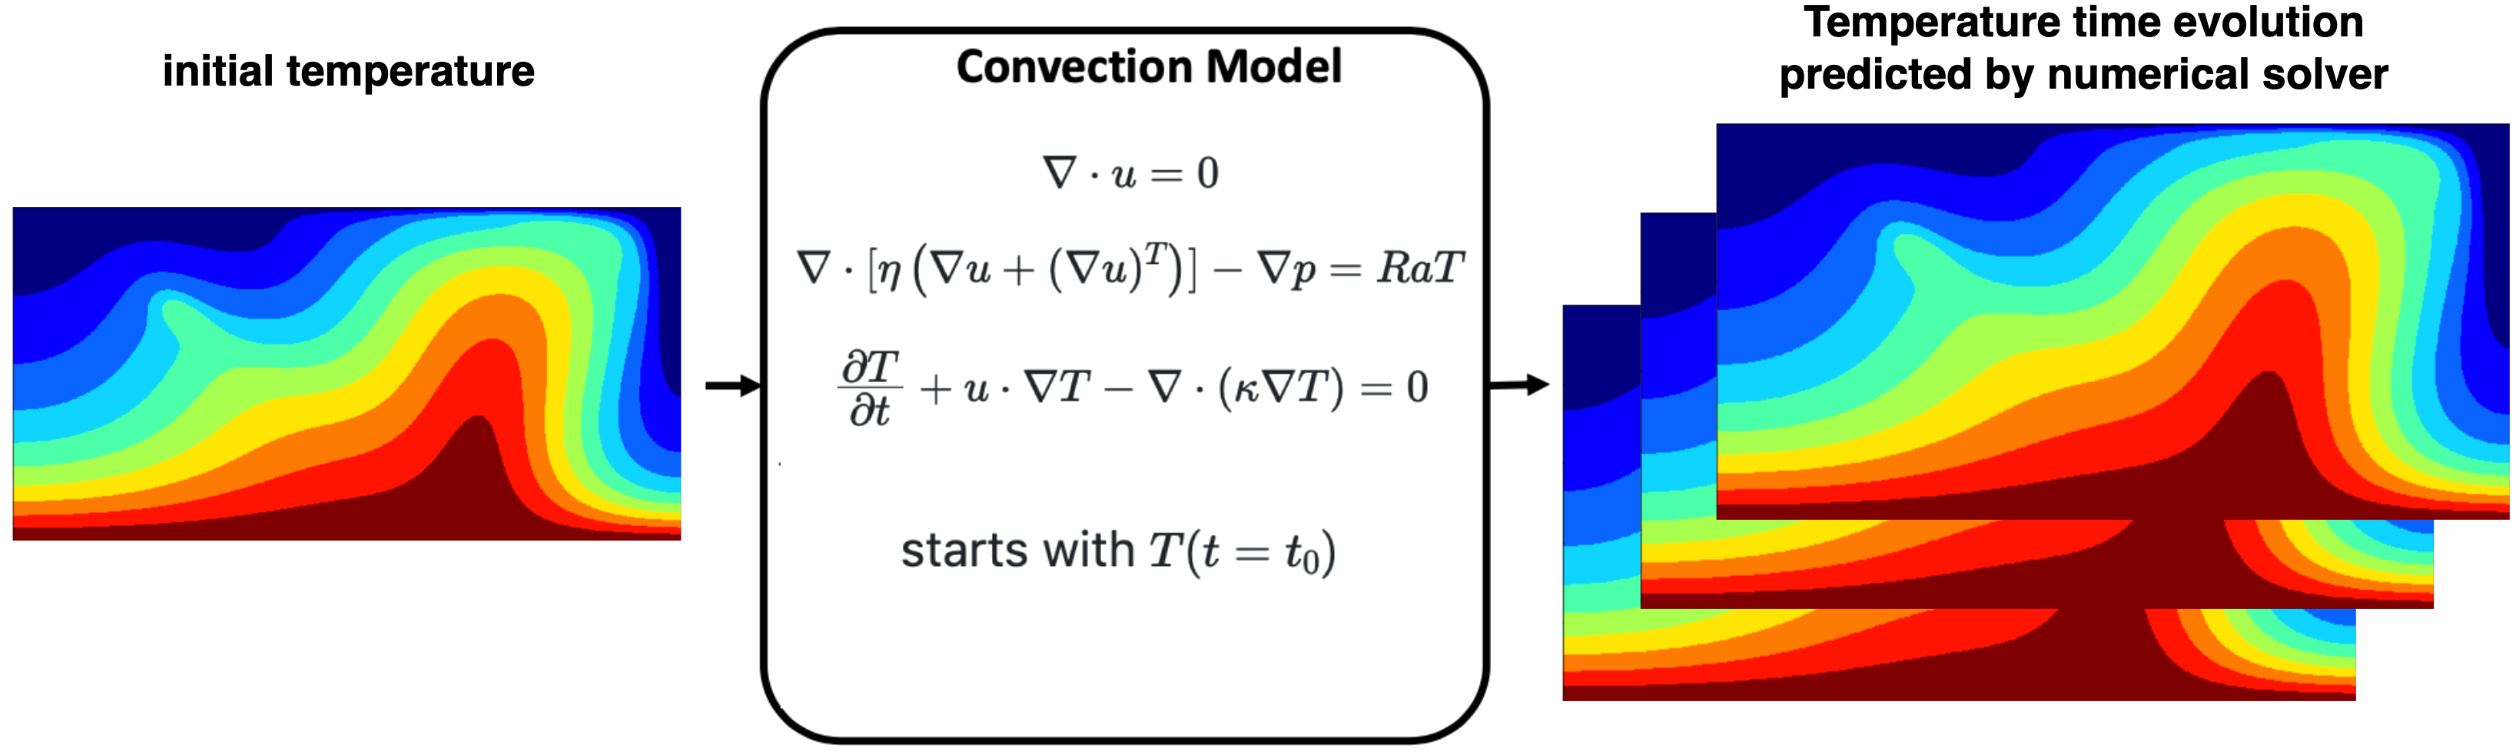
\includegraphics[scale=0.15]{figures/mantle_convection_images/Mantle_Convection_workflow.png}
    \label{figure:MC_workflow}
\end{figure}

To explore the usage of Neural Networks as surrogate models for the original mantle convection numerical solver with the aim of significantly reducing computational demands, three different datasets are tested, which we refer to as  ``Limited Dataset'', ``Larger Dataset'' and ``Interpolated Dataset''. Each dataset is composed of several temperature time-series with 100 timestamps each resulting from numerical simulations with randomly sampled initial conditions (except for the Interpolated Dataset, which is created from the Larger Dataset using interpolation).

\section{Mantle Convection Simulation on Limited Dataset}

The limited dataset consists of 100 files.  Each of these files represents one mantle convection simulation with 100 time steps generated from an initial condition with random number of points and random amplitude and coordinates of Gaussian anomalies distributed in space. We thus have a total of 10,000 temperature fields in the Limited Dataset. Starting from each initial condition, we convect as long as there is meaningful change in the simulation (that is the temperature fields change enough after one time-step). The size of each temperature field is $201 \times 401$. The time step is adaptive, otherwise the whole random generation of the initial condition would be hard to implement. These adaptive timestamps lead to a problem, that is, the distance between each consecutive pairs of time steps might not be the same even within the same simulation file of the data set. This could lead to some uncommon behaviors when predicting a sequence of temperature fields using the ML architecture, which will be discussed in more detail in the following sections.

Figure \ref{figure:temperature_field_sample} shows one randomly selected temperature field in the dataset with the $y$-axis inverted and colored using a 10-color-map. All figures in this chapter will have their $y$-axis inverted and colored using this very same 10-color-map, but without labels on $x$-axis and $y$-axis, nor color-map, for conciseness.

\begin{figure}[H]
    \caption{Temperature Field example. (For the colorbar of the upcoming figures, see this one.)}
    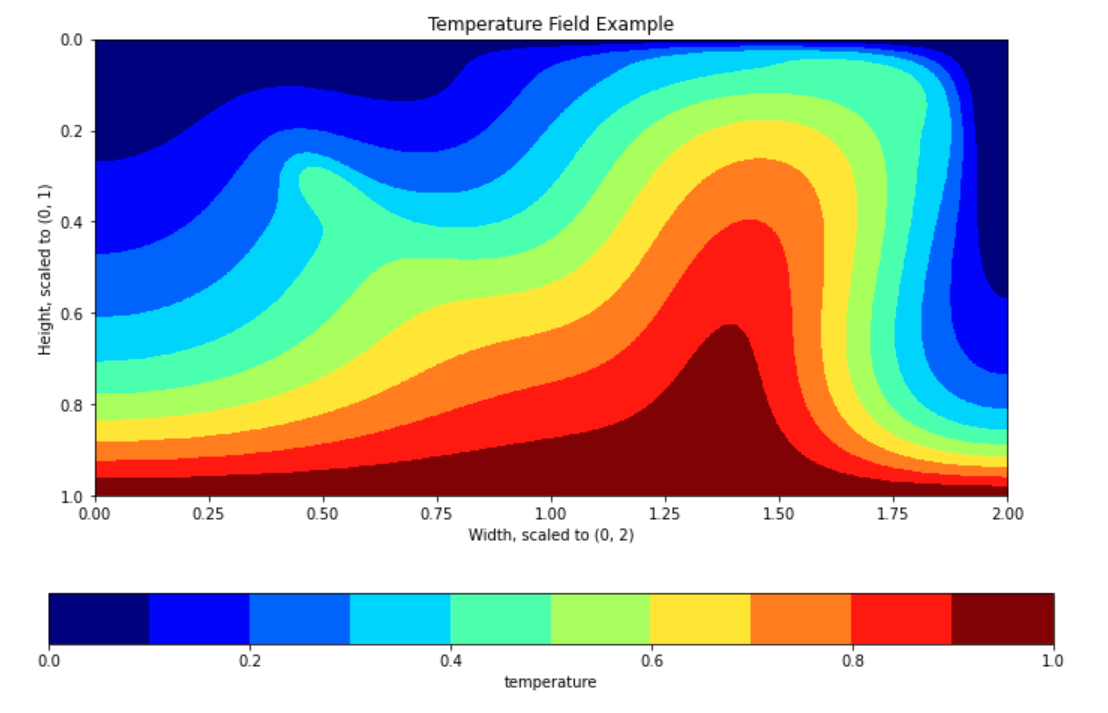
\includegraphics[scale=0.6]{figures/mantle_convection_images/temperature_field_example.png}
    \label{figure:temperature_field_sample}
\end{figure}

The entire dataset is randomly divided using a ratio of 8:1:1, where 80 per cent of the dataset is used for training, 10 per cent for testing, and the remaining 10 per cent to perform validation and prevent overfitting. However, the way we divide them is different for ConvAE, FNN and LSTM. This will be discussed in more detail in the following sections.

The dataset is uploaded to Gadi, an HPC system, for additional storage, and to further accelerate the training process using Graphic Processing Units (GPUs). 

\subsection{Compression of temperature fields}

Since applying Machine Learning (ML) algorithms directly on the original sized temperature fields can take significantly more time to train the model and could potentially lead to over-parameterization, we decided to compress the temperature fields first before feeding the data into the different ML architectures.

In this study, the overall process to solve the mantle convection problem is: 
\begin{enumerate}
  \item Train the ConvAE.
  \item Train the FNN/LSTM using the latent space representation of both input and output data. (Encoder from ConvAE is used to get the latent space representation.)
  \item Evaluate the predicted temperature in its original size. (Decoder from ConvAE is used to get the original sized temperature from its latent space representation.)
\end{enumerate}

Figures \ref{figure:ConvAE_workflow}, \ref{figure:FNN_workflow} and \ref{figure:LSTM_workflow} 
below illustrate the workflow for ConvAE, FNN and LSTM, respectively.

\begin{figure}[H]
    \centering
    \caption{Workflow for ConvAE.}
    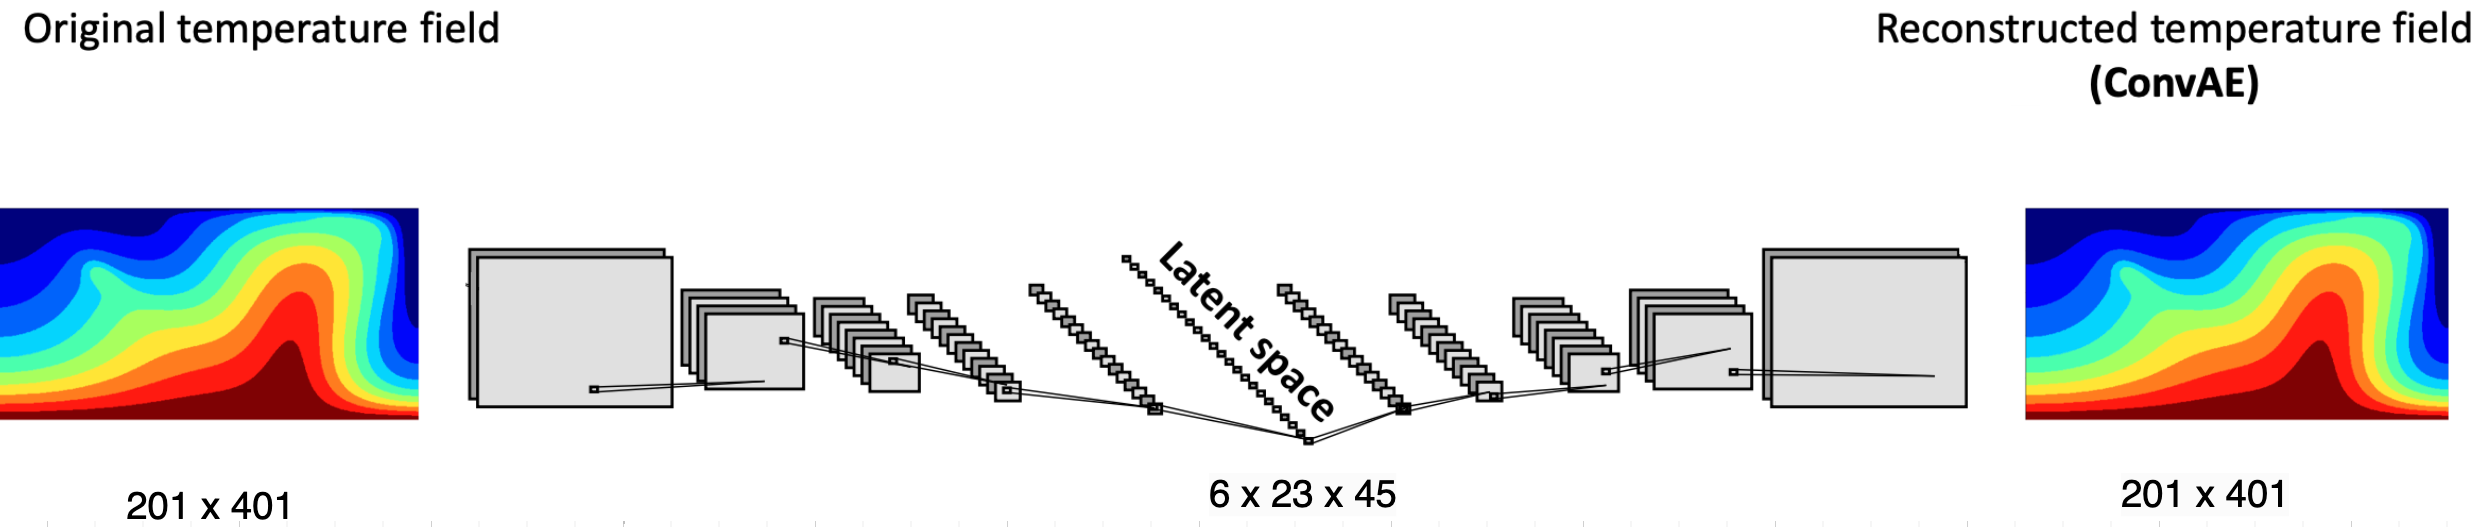
\includegraphics[scale=0.3]{figures/mantle_convection_images/ConvAE_workflow.png}
    \label{figure:ConvAE_workflow}
\end{figure}

\begin{figure}[H]
    \centering
    \caption{Workflow for FNN.}
    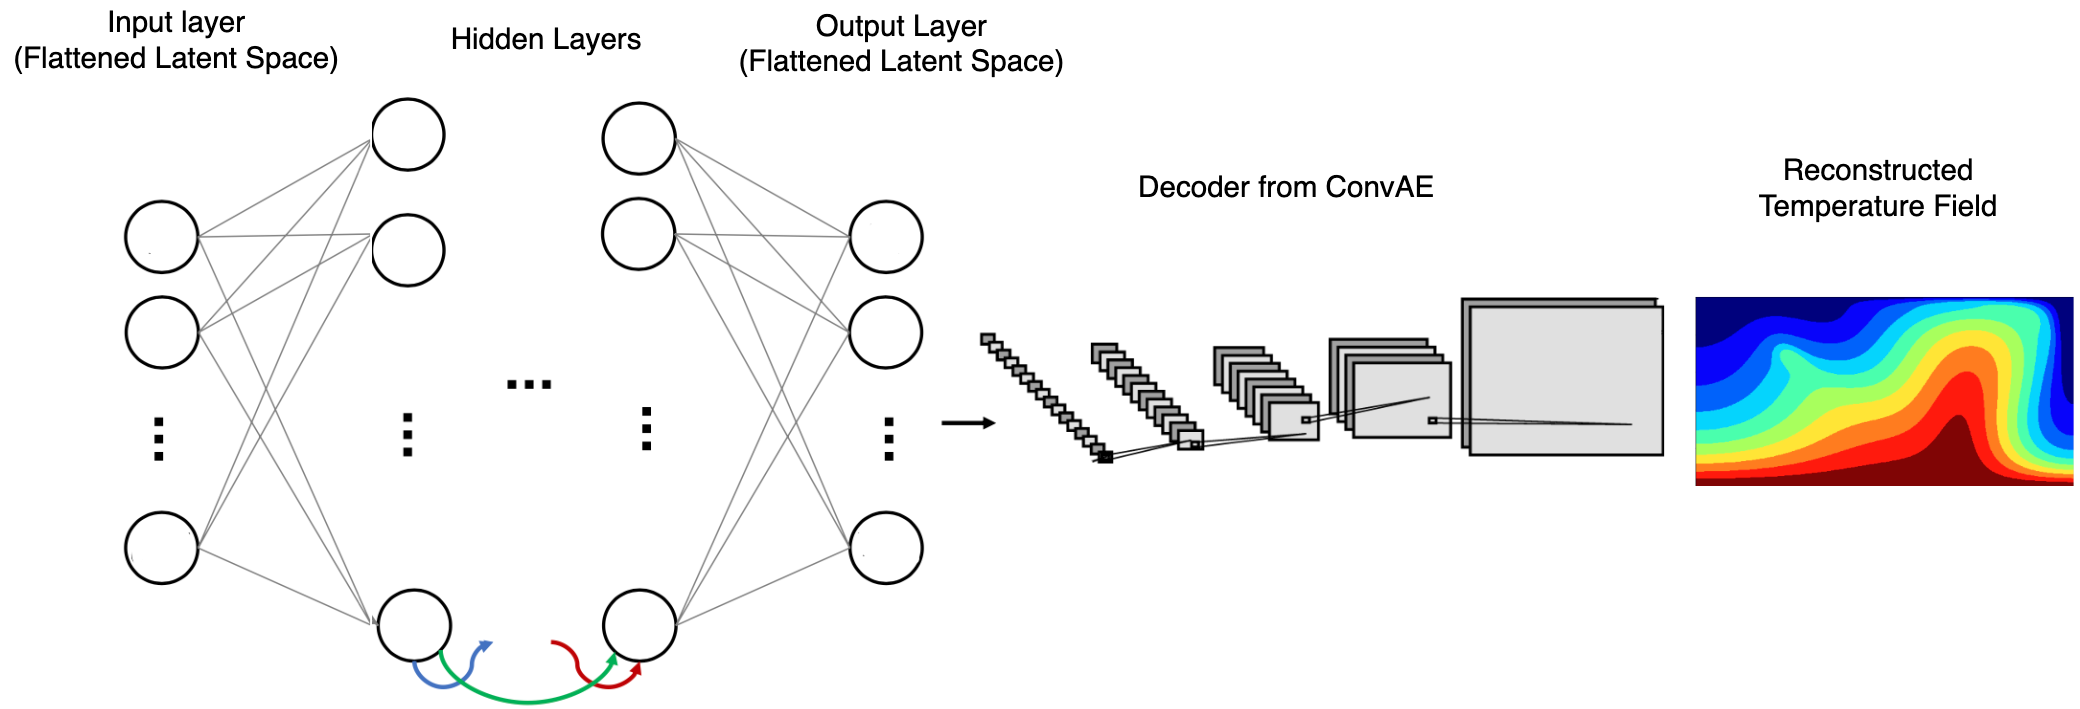
\includegraphics[scale=0.35]{figures/mantle_convection_images/FNN_workflow.png}
    \label{figure:FNN_workflow}
\end{figure}

\begin{figure}[H]
    \centering
    \caption{Simple Workflow for LSTM. Tn represents a temperature field in its latent space representation. Here we input the first 50 temperature fields (once compressed and flattened) from a simulation into the LSTM and LSTM  predicts the remaining 50 temperature fields of the same simulation (also compressed and flattened). Source of the left figure: StackOverflow.}
    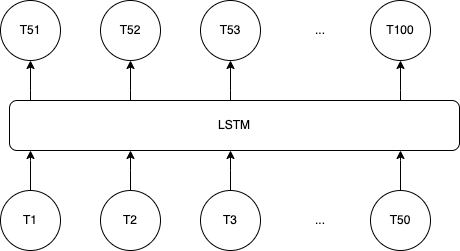
\includegraphics[scale=0.6]{figures/mantle_convection_images/LSTM_workflow.png}
    \label{figure:LSTM_workflow}
\end{figure}

The complete set of 10,000 temperature fields are randomly shuffled and divided using a ratio of 80\%, 10\%, 10\% for training, testing and validation, respectively, where each piece of data consists of only one temperature field (fed as both the input and output during training and testing). Given the size of the training set, ConvAE is fed with a batch size of 16 temperature fields during training via Mini-Batch Gradient Descent.

We find that ConvAE with a latent space size of $6 \times 23 \times 45$ offers an excellent compression factor of 13 while being able to reconstruct the temperature fields in its original size with the lowest data loss on the test set.

The architecture of the ConvAE in this case consists of two convolutional layers for the encoder and two transpose convolutional layers for the decoder. Both of these four layers use a filter of size $5 \times 5$ and a stride of $3 \times 3$. Tanh() is used as the activation function to introduce non-linearity between each layers (except for the last layer in the decoder) and mean square error (MSE) is used as the loss function. The model is trained for 1,000 epochs on Gadi.

In the following figures, we present some detailed test results for this ConvAE, including the training and validation losses in Figure \ref{figure:ConvAE_limited_losses}, overall testing result in Figure \ref{figure:ConvAE_limited_testing}, and the most/least accurate prediction in 
Figure \ref{figure:ConvAE_limited_best_worst}.

\begin{figure}[H]
    \caption{Training and validation losses of ConvAE trained with Limited Dataset.}
    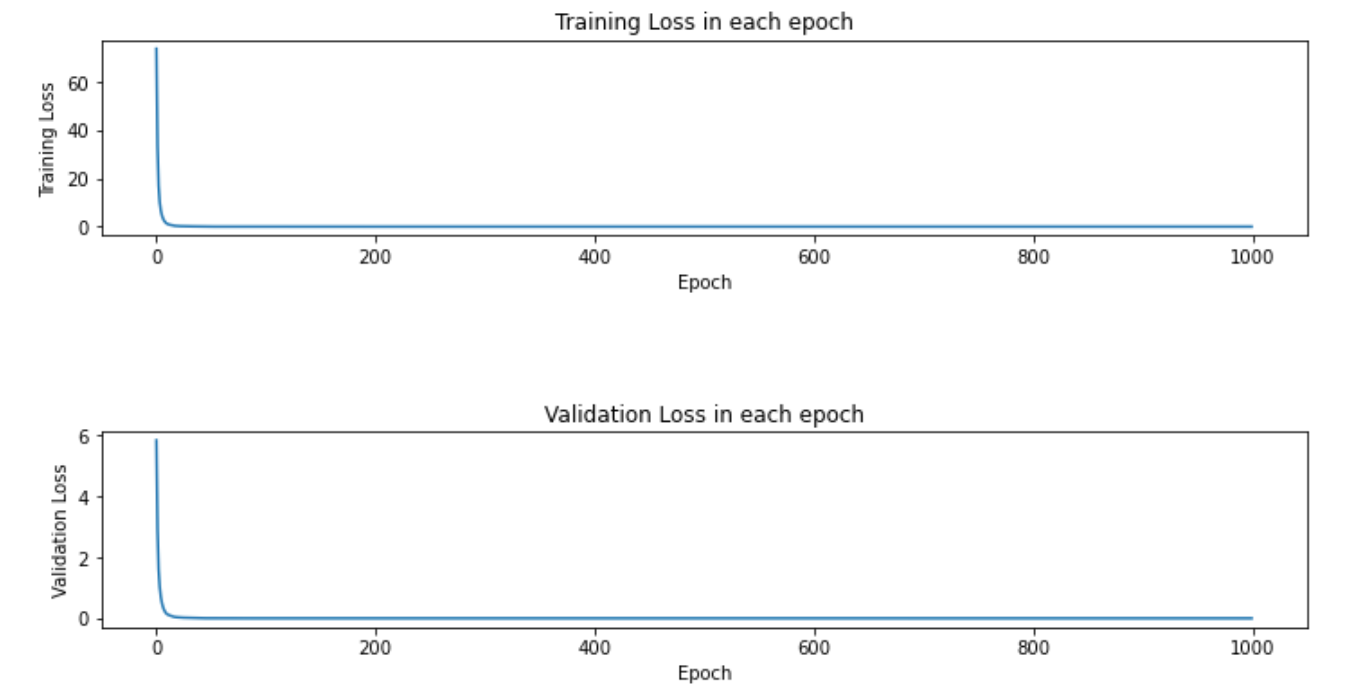
\includegraphics[scale=0.6]{figures/mantle_convection_images/limited_dataset/ConvAE_trainingData.png}
    \label{figure:ConvAE_limited_losses}
\end{figure}

\begin{figure}[H]
    \caption{Overall testing result of ConvAE trained with Limited Dataset.}
    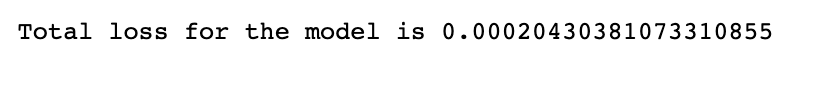
\includegraphics[scale=0.8]{figures/mantle_convection_images/limited_dataset/ConvAE_OverallTesting.png}
    \label{figure:ConvAE_limited_testing}
\end{figure}

\begin{figure}[H]
\centering
\begin{subfigure}{0.45\textwidth}
    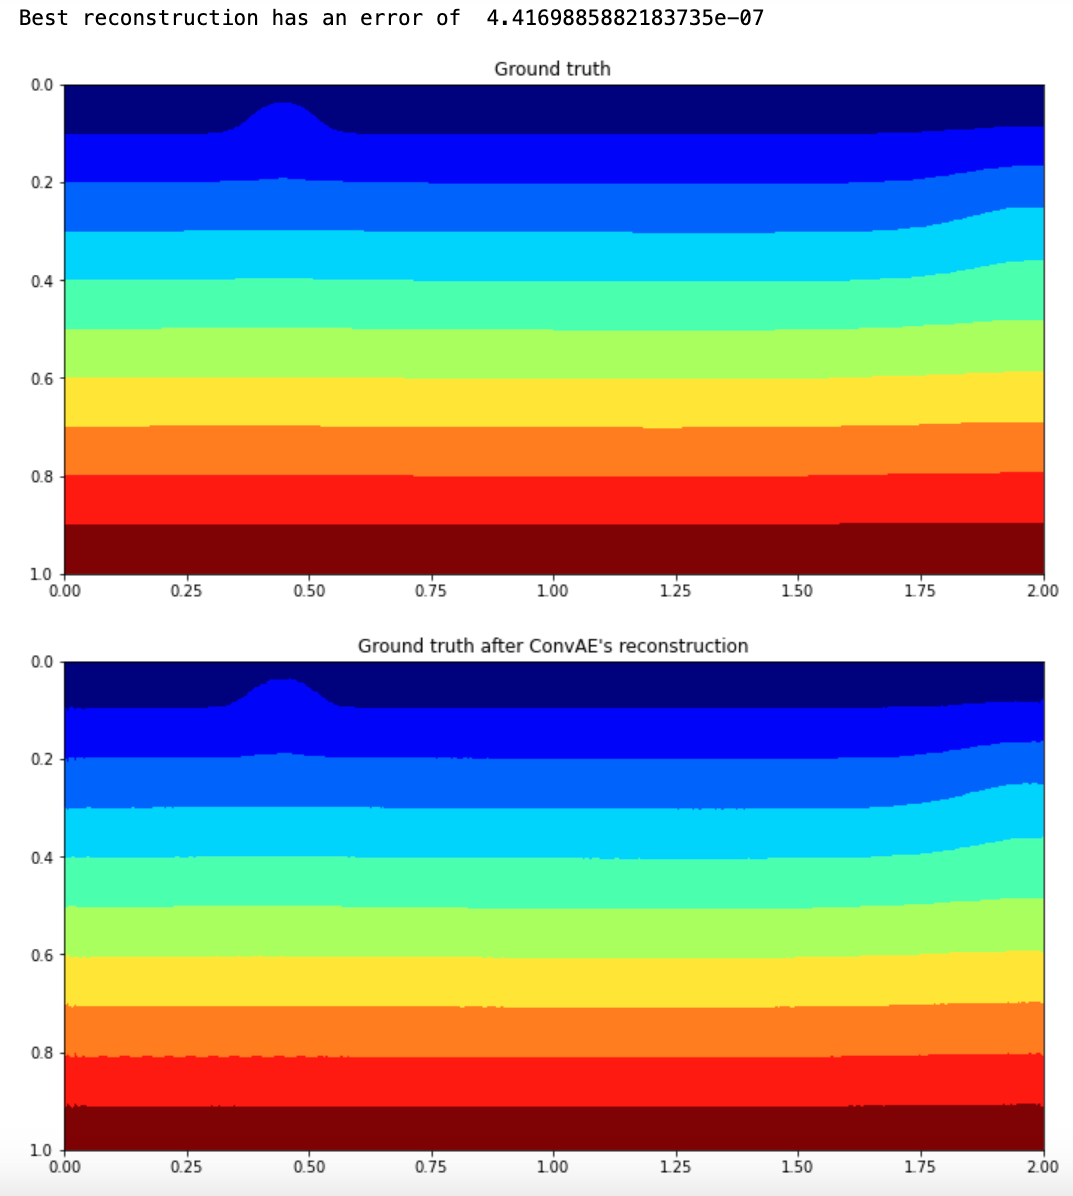
\includegraphics[width=\textwidth]{figures/mantle_convection_images/limited_dataset/ConvAE_Best.png}
    \caption{Most accurate reconstruction of ConvAE trained with Limited Dataset.}
\end{subfigure}
\hfill
\begin{subfigure}{0.45\textwidth}
    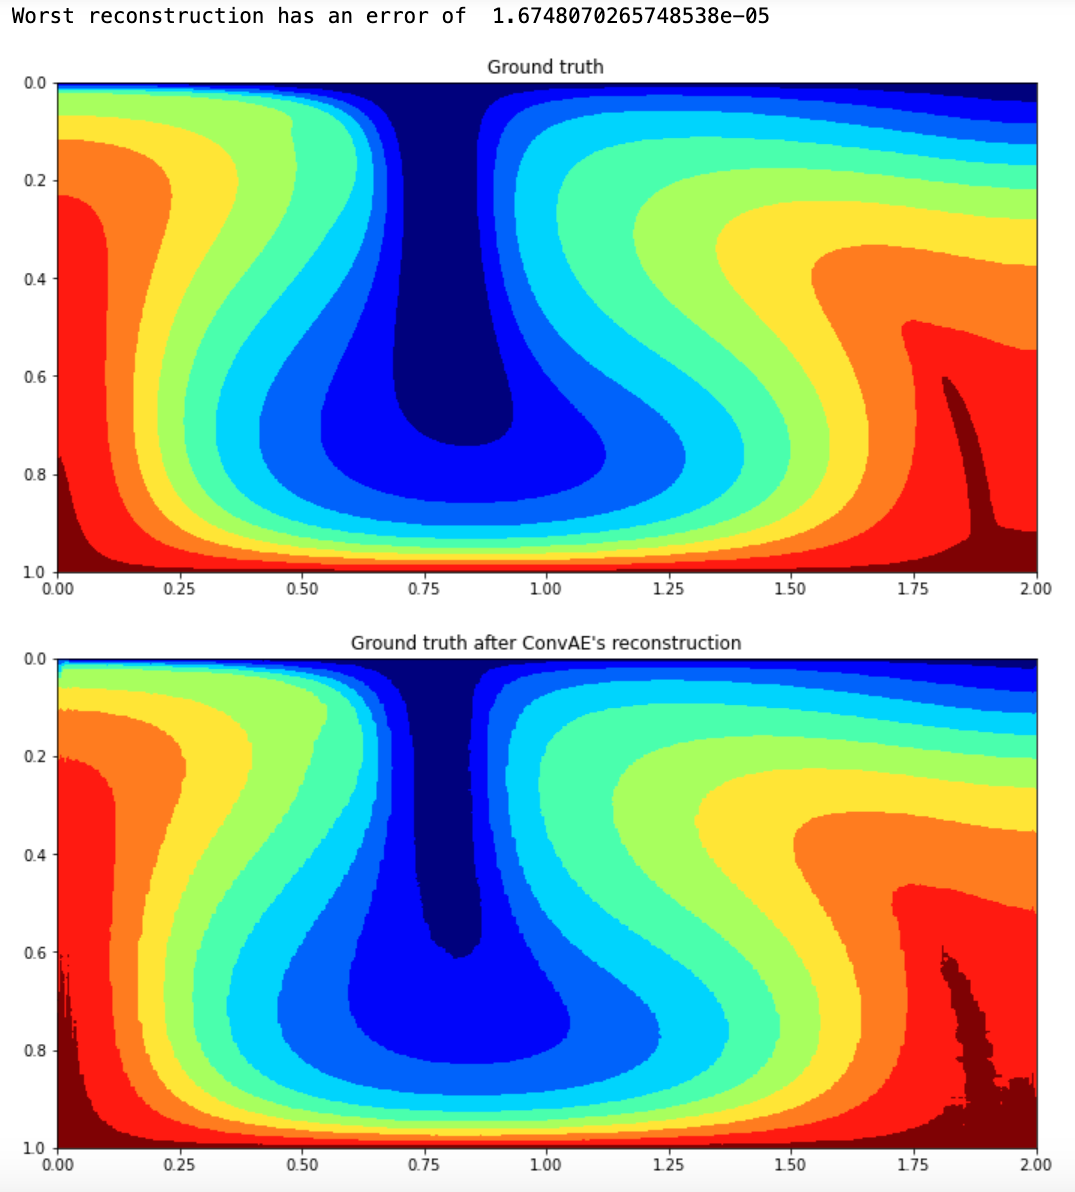
\includegraphics[width=\textwidth]{figures/mantle_convection_images/limited_dataset/ConvAE_Worst.png}
    \caption{Least accurate reconstruction of ConvAE trained with Limited Dataset.}
\end{subfigure}     
\caption{Best case and worst case using ConvAE.}
\label{figure:ConvAE_limited_best_worst}
\end{figure}


On average, the reconstruction loss is low and no overfitting occurs. However, we can observe that the ConvAE does not reconstruct the thin feature in the bottom right corner of the worst case. This could imply that the ConvAE works best for ``smooth'' input hence others with small scale length features will generally perform worse.

We also performed POD (Proper Orthogonal Decomposition) analysis to the compressed-decompressed fields with contrast to the original temperature fields, and the results are remarkable as well. The results of this analysis will be presented in the following sections and contrasted to the POD analysis of the prediction model (FNN or LSTM).


\subsection{Fully Connected Neural Network for Prediction}

We now move on to predict the latent space representation and our first candidate is the feed-forward fully connected neural network (FNN). The FNN in this study uses each adjacent pair of temperature fields (e.g. $i$-th and ($i+1$)-th fields) as one training set, takes one temperature field as the input and outputs the temperature field at the next time step. Therefore, the dataset is reconstructed into 9,900 pairs of temperature fields with consecutive timestamps. These pairs are randomly shuffled and divided in a ratio of 80\%, 10\%, 10\% for training, testing and validation, respecively, where each piece of data consists of two temperature fields having consecutive timestamps.

Before the latent space representation is fed as the input of FNN, it is flattened into one dimension. The prediction result of FNN in this case is then resized from a one dimensional vector ($1 \times 6210$) to the shape of the latent space ($6 \times 23 \times 45$) before we applied further processing.

The trainable parameters of the FNN are optimized using small mini-batches of 16 pairs of consecutive temperature fields and Adam as the optimizer, where the loss function is defined as the mean square error (MSE) between the prediction of the FNN and the actual output (both in the shape of latent space representation, which is $6 \times 23 \times 45$).

After testing with FNNs that have different number of hidden layers and neurons per hidden layer, we found that architectures with a total number 3 hidden layers seemed to perform the best. We also tested some deeper architectures with 4-5 hidden layers. However, there is no significant reduction in the loss value.

In the following figures, we present results from a FNN with 3 hidden layers with 3,105; 1,035; and 3,105 neurons per layer, respectively. Tanh() was used as activation function. The network was trained for 1,000 epochs. The results reported include the training and validation losses in Figure \ref{figure:FNN_limited_losses}, overall testing result in Figure \ref{figure:FNN_limited_testing}, and the most/least accurate prediction in Figures \ref{figure:FNN_limited_best} and \ref{figure:FNN_limited_worst}, respectively.

\begin{figure}[H]
    \caption{Training and validation losses of FNN trained with Limited Dataset.}
    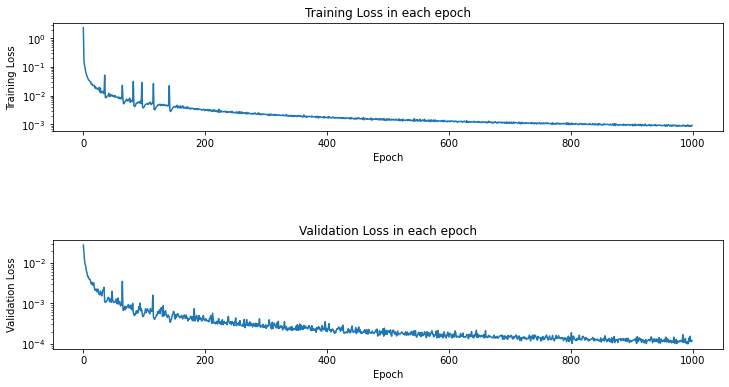
\includegraphics[scale=0.6]{figures/mantle_convection_images/limited_dataset/FNN_trainingData.png}
    \label{figure:FNN_limited_losses}
\end{figure}

\begin{figure}[H]
    \caption{Overall testing result of FNN trained with Limited Dataset.}
    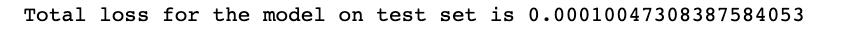
\includegraphics[scale=0.8]{figures/mantle_convection_images/limited_dataset/FNN_OverallTesting.png}
    \label{figure:FNN_limited_testing}
\end{figure}

\begin{figure}[H]
    \caption{Ground truth, ground truth after ConvAE's compression-decompression, and most accurate prediction of FNN trained with Limited Dataset.}
    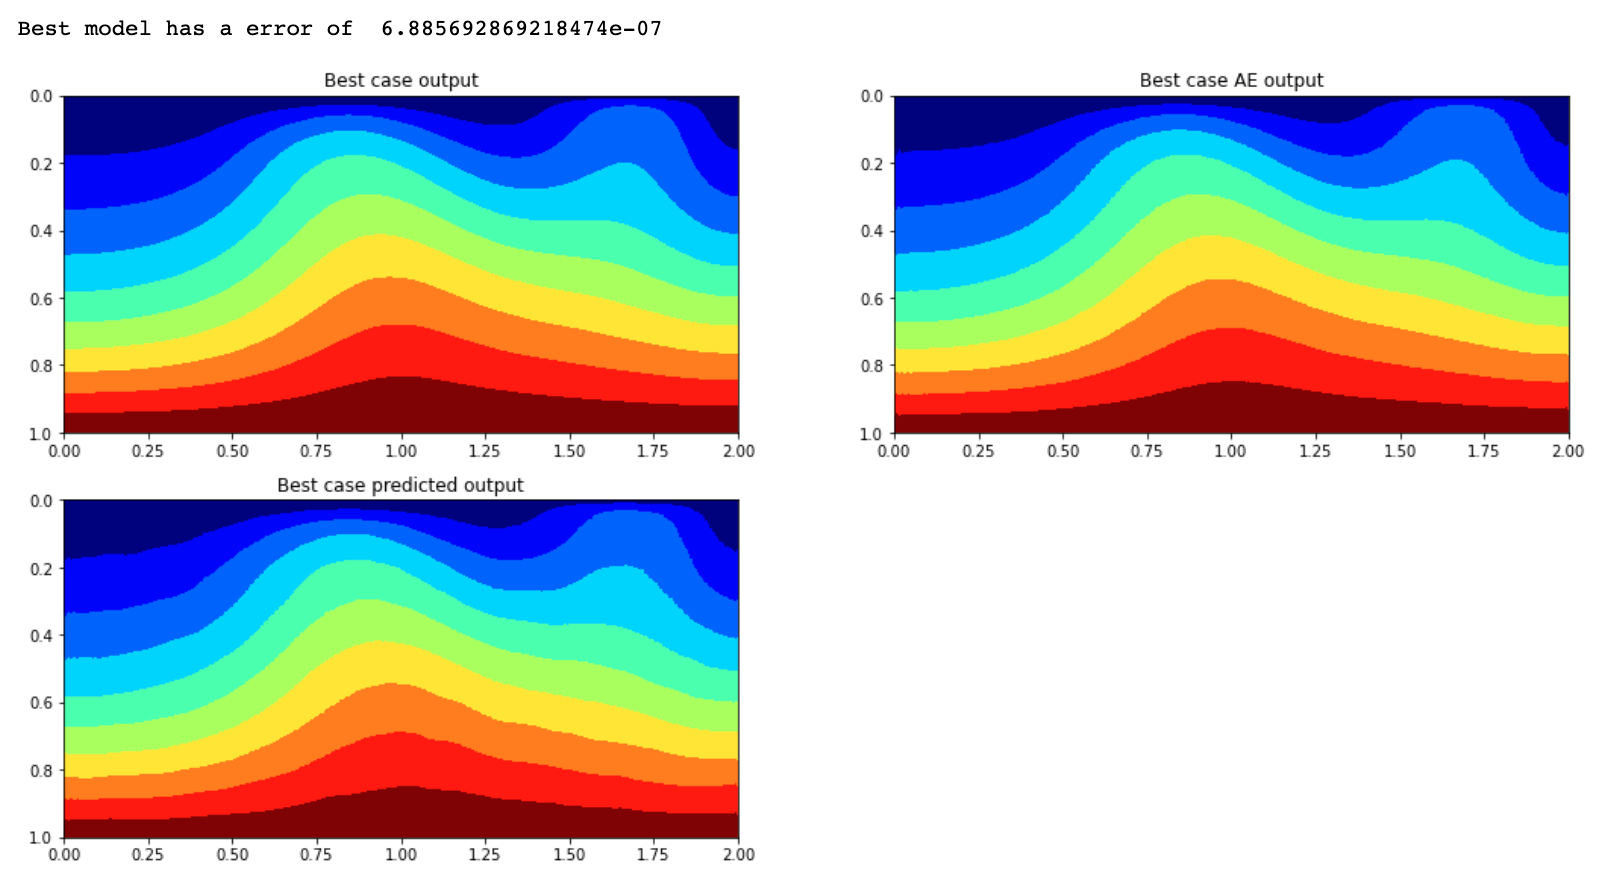
\includegraphics[scale=0.5]{figures/mantle_convection_images/limited_dataset/FNN_Best.png}
    \label{figure:FNN_limited_best}
\end{figure}

\begin{figure}[H]
    \caption{Ground truth, ground truth after ConvAE's compression-decompression, and least accurate prediction of FNN trained with Limited Dataset.}
    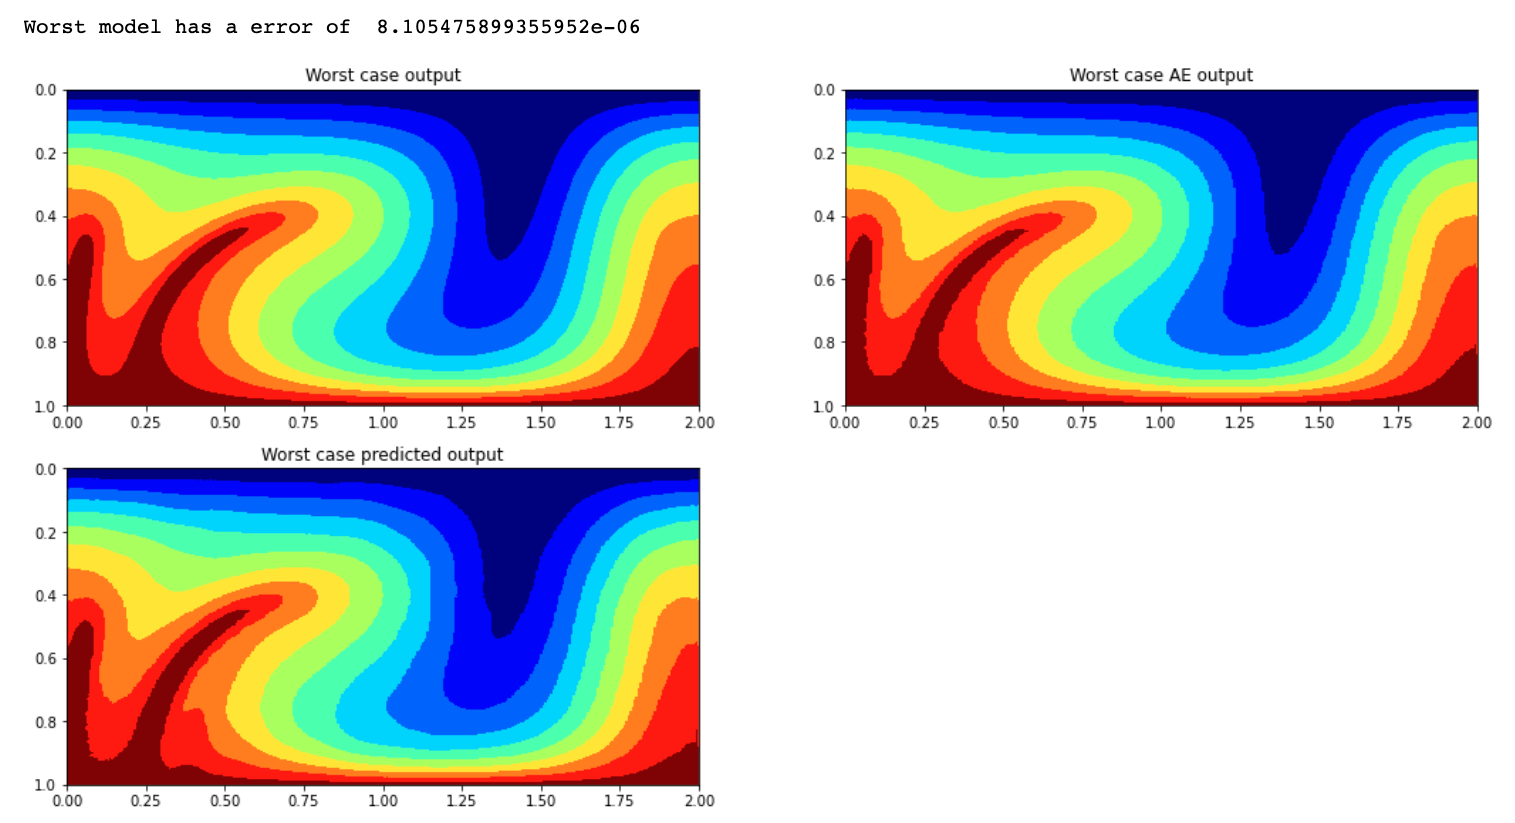
\includegraphics[scale=0.5]{figures/mantle_convection_images/limited_dataset/FNN_Worst.png}
    \label{figure:FNN_limited_worst}
\end{figure}

On average, the loss values are low and no overfitting occurs. The prediction for the temperature field at the next time step is able to capture the main features precisely with some small information loss, which is partially due to information loss caused by the compression-decompression process of ConvAE.

To further evaluate the performance of FNN in predicting a complete time series, two methods are tested on all 100 simulations one by one: 

\begin{enumerate}
  \item ``One-for-All'' (also referred as ``Output-as-input Prediction''): Only take the first temperature field in the file as the input and use a prediction-as-input loop to get the rest of the 99 temperature fields. (use $T1$ from dataset $\rightarrow$ get predicted $T2$ $\rightarrow$ use predicted $T2$ $\rightarrow$ get predicted $T3$ $\rightarrow$ ...)
  \item ``One-for-One'' (also referred as ``Single Prediction''): Constantly feed a temperature field from the original dataset and get the temperature field at the next time step as usual. (use $T1$ from dataset $\rightarrow$ get predicted $T2$ $\rightarrow$ use $T2$ from dataset $\rightarrow$ get predicted $T3$ $\rightarrow$ ...)
\end{enumerate}

The first method can reduce the computational demands of the mantle convection problem more effectively than the second method, since we only need one initial input data and the model can generate the rest of the temperature field sequence. Therefore, the following best case and worst case will be evaluated using the data loss of the first method.

To better visualize the prediction result of the above two methods, two animations representing the best and worst cases (evaluated based on the sum of MSE for each prediction using the first method) are generated. From top to bottom, the first picture represents the actual output from the dataset, the second one represents the prediction result using the first method, and the last one represents the prediction result using the second method.

Figure \ref{figure:FNN_limited_best_gif} and \ref{figure:FNN_limited_worst_gif} show 10\% of the two sprite sheets extracted from the animation (every 10th frame) for reading convenience.

\begin{figure}[H]
    \centering
    \caption{Best case animation sheet of FNN trained with Limited Dataset (Link to animation: \url{https://drive.google.com/file/d/1Hmb4UlevBHMRw0jDScTwUzDFPbYNubKO/view?usp=sharing})}
    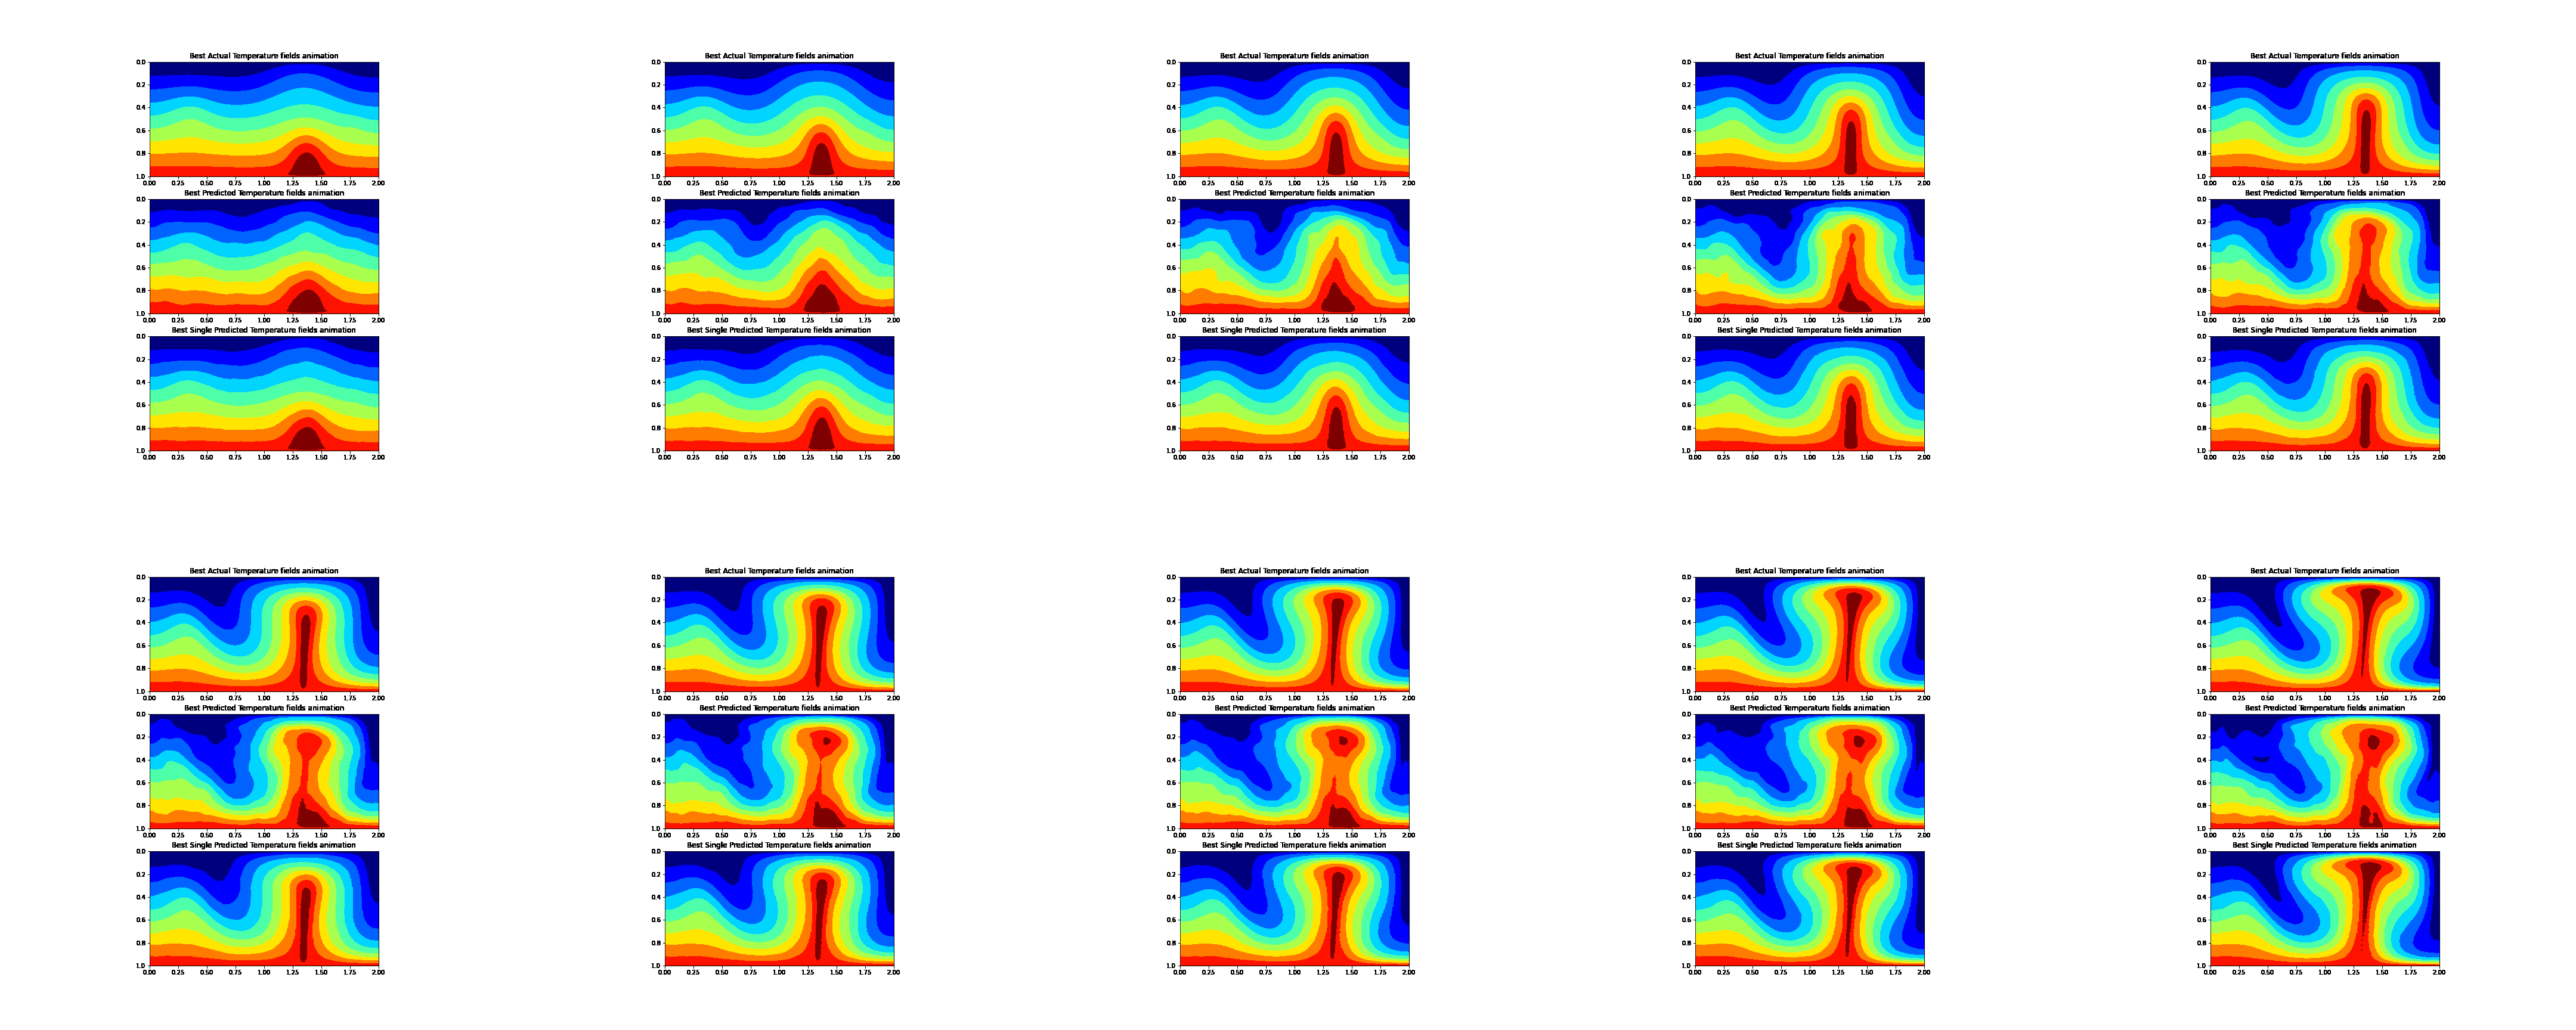
\includegraphics[scale=0.10]{figures/mantle_convection_images/limited_dataset/FNN_Best_GIF_sheet.png}
    \label{figure:FNN_limited_best_gif}
\end{figure}

\begin{figure}[H]
    \centering
    \caption{Worst case animation sheet of FNN trained with Limited Dataset (Link to animation: 
    \url{https://drive.google.com/file/d/11jRFxq-XuIUvTk74OuxswDn3u031k_q7/view?usp=sharing})}
    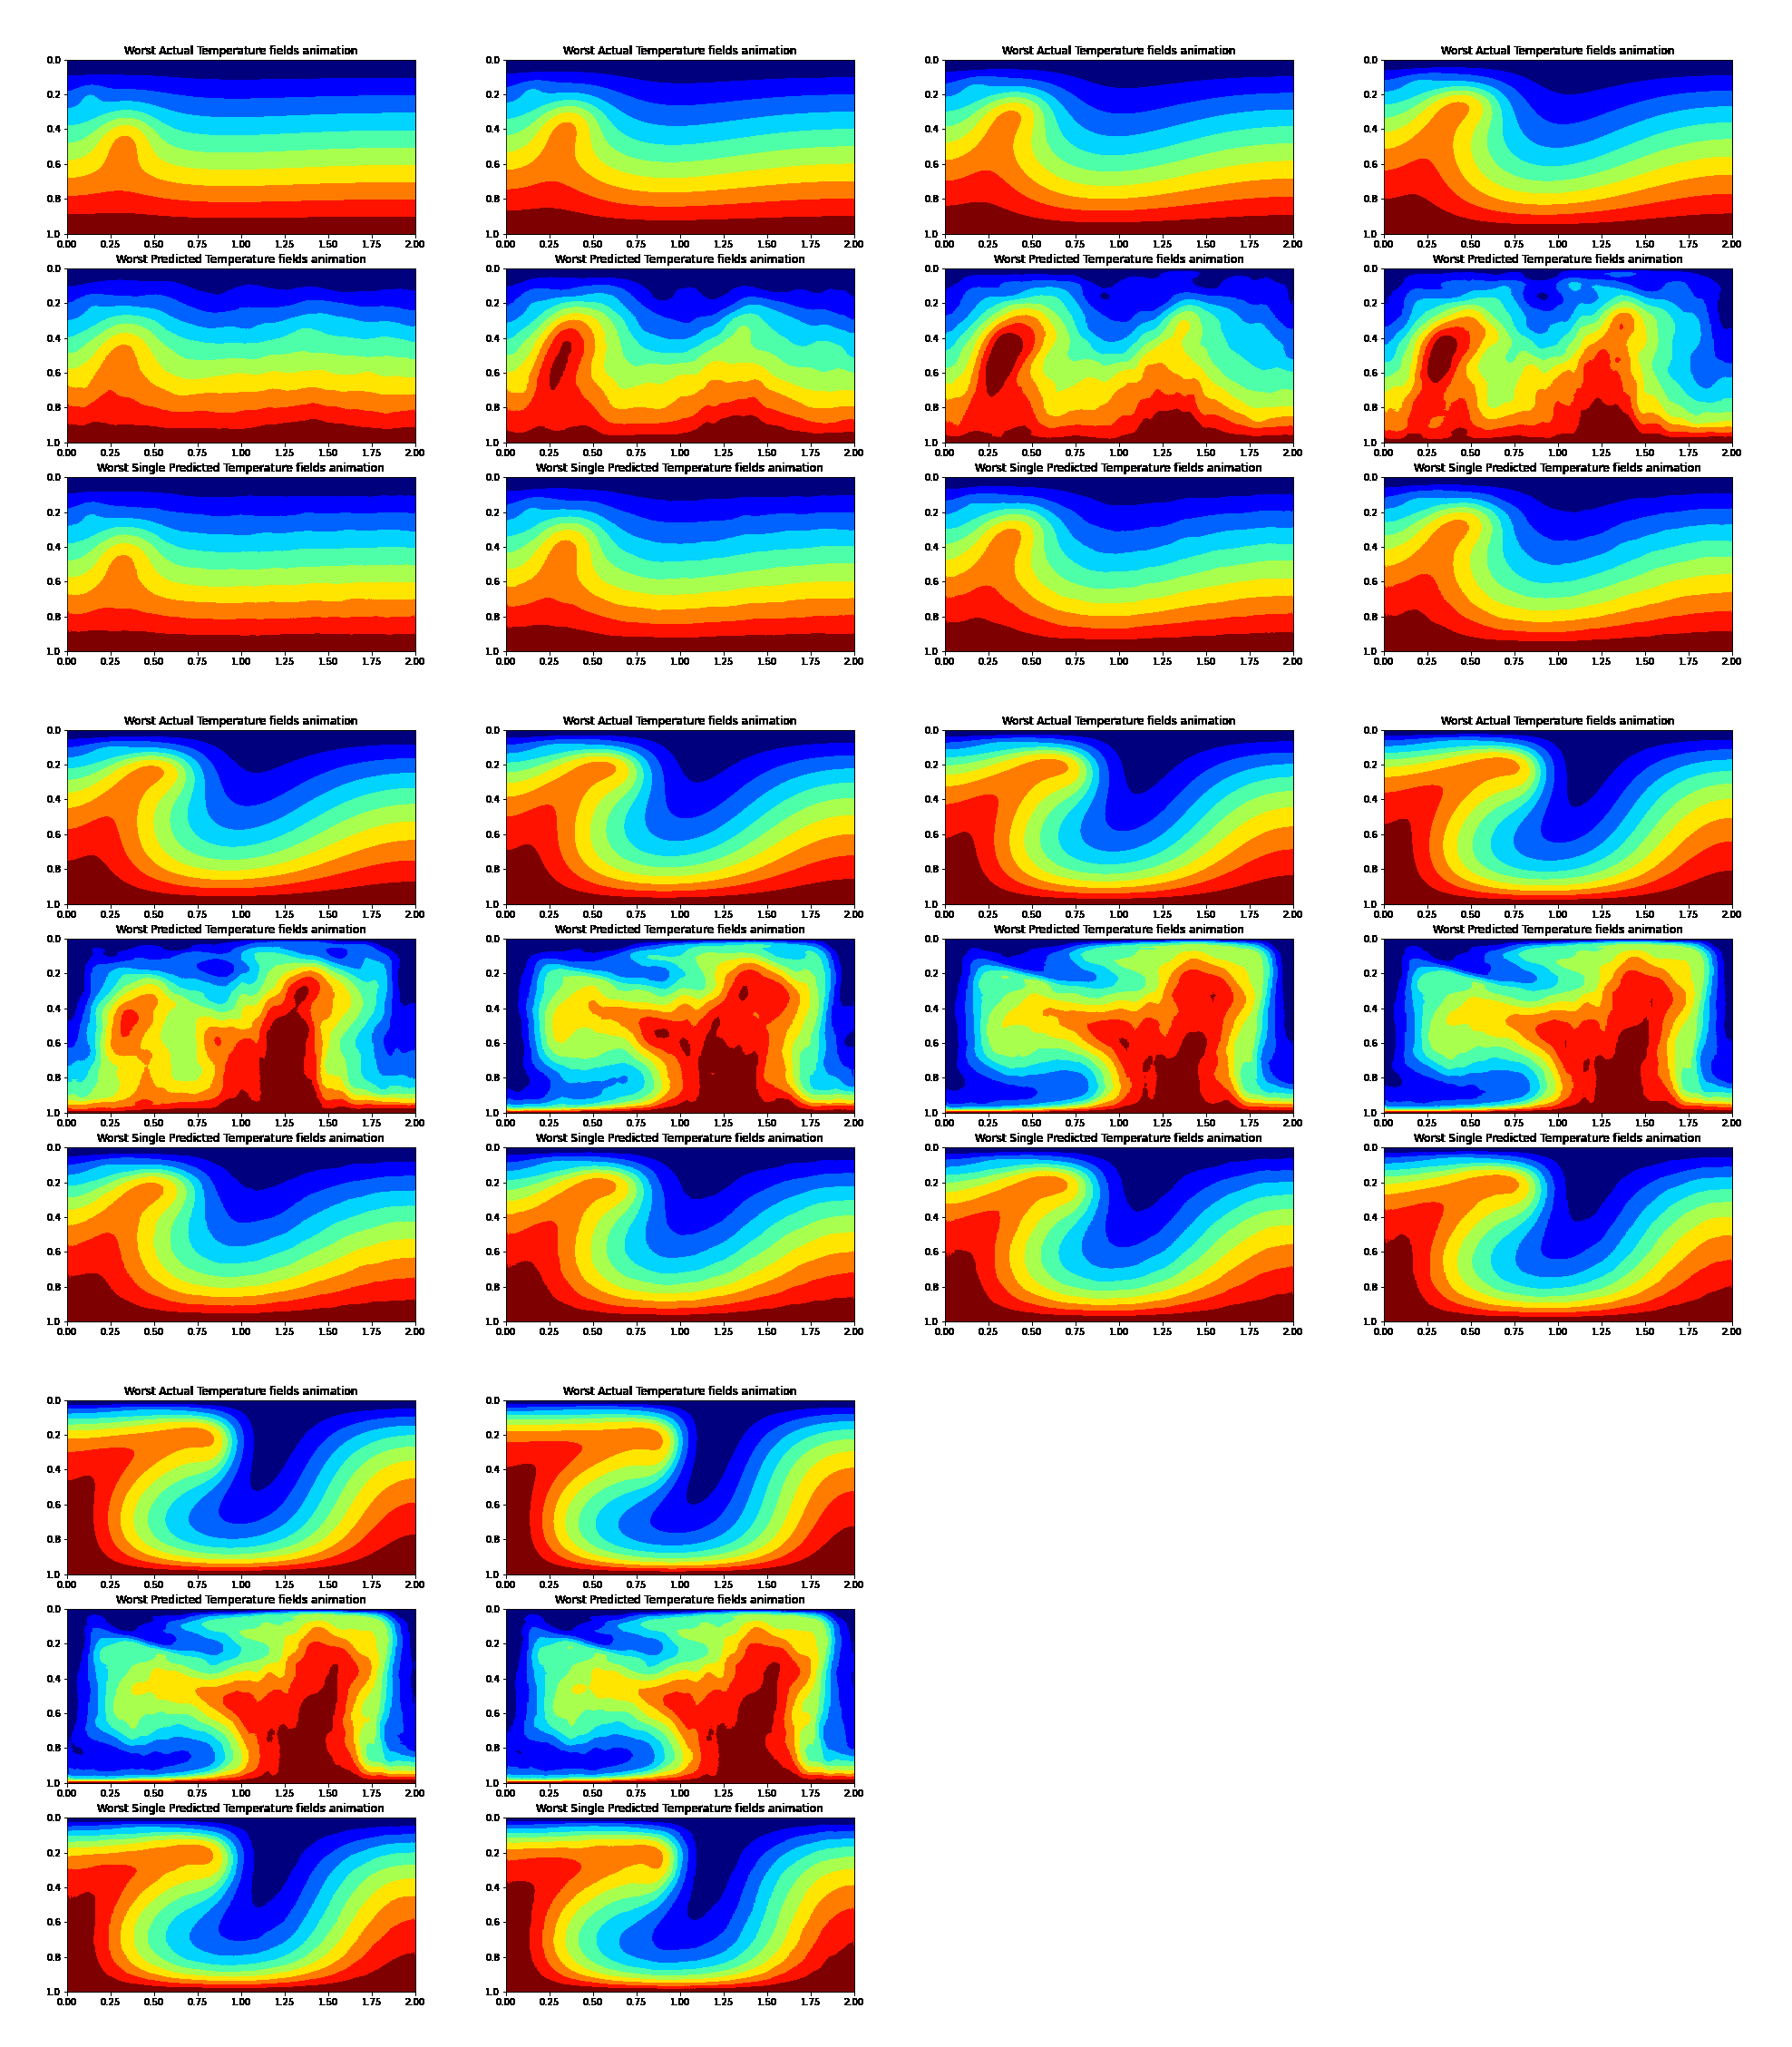
\includegraphics[scale=0.10]{figures/mantle_convection_images/limited_dataset/FNN_Worst_GIF_sheet.png}
    \label{figure:FNN_limited_worst_gif}
\end{figure}

To further evaluate the performance of these two methods, we applied a technique called Proper Orthogonal Decomposition (POD) to their predictions in both the best and worst cases. We also consider the original ``ground-truth'' time series and the compressed-decompressed version generated by ConvAE to serve as a contrast.

POD is mainly used to decompose a physical field (e.g., temperature field) depending on the different variables that influence its physical behaviors and it is similar to Principle Component Analysis (PCA) since it refers to eigenvalues of a physical field.\citep{10.1146_annurev.fl.25.010193.002543}. The Singular Value Decomposition (SVD) of a simulation matrix $X$ (spatial points $\times$ time-steps, in this case $201 \times 401 \times 100$) is computed as \citep{10.1515_9783110671490-007}:
\begin{equation}
X = U\Sigma V,
\end{equation}
where the diagonal of $\Sigma$ contains the eigenvalues (POD coefficients) for this simulation.

Figure \ref{figure:FNN_limited_best_POD} and \ref{figure:FNN_limited_worst_POD} show the POD results when applied to the best and worst cases predictions, respectively.

\begin{figure}[H]
    \caption{Best case POD of FNN trained with Limited Dataset.}
    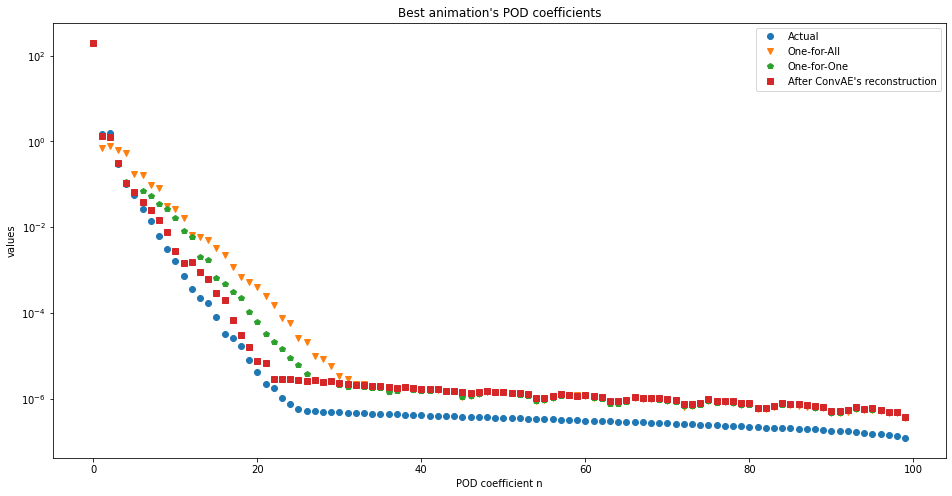
\includegraphics[scale=0.5]{figures/mantle_convection_images/limited_dataset/FNN_Best_POD.png}
    \label{figure:FNN_limited_best_POD}
\end{figure}

\begin{figure}[H]
    \caption{Worst case POD of FNN trained with Limited Dataset.}
    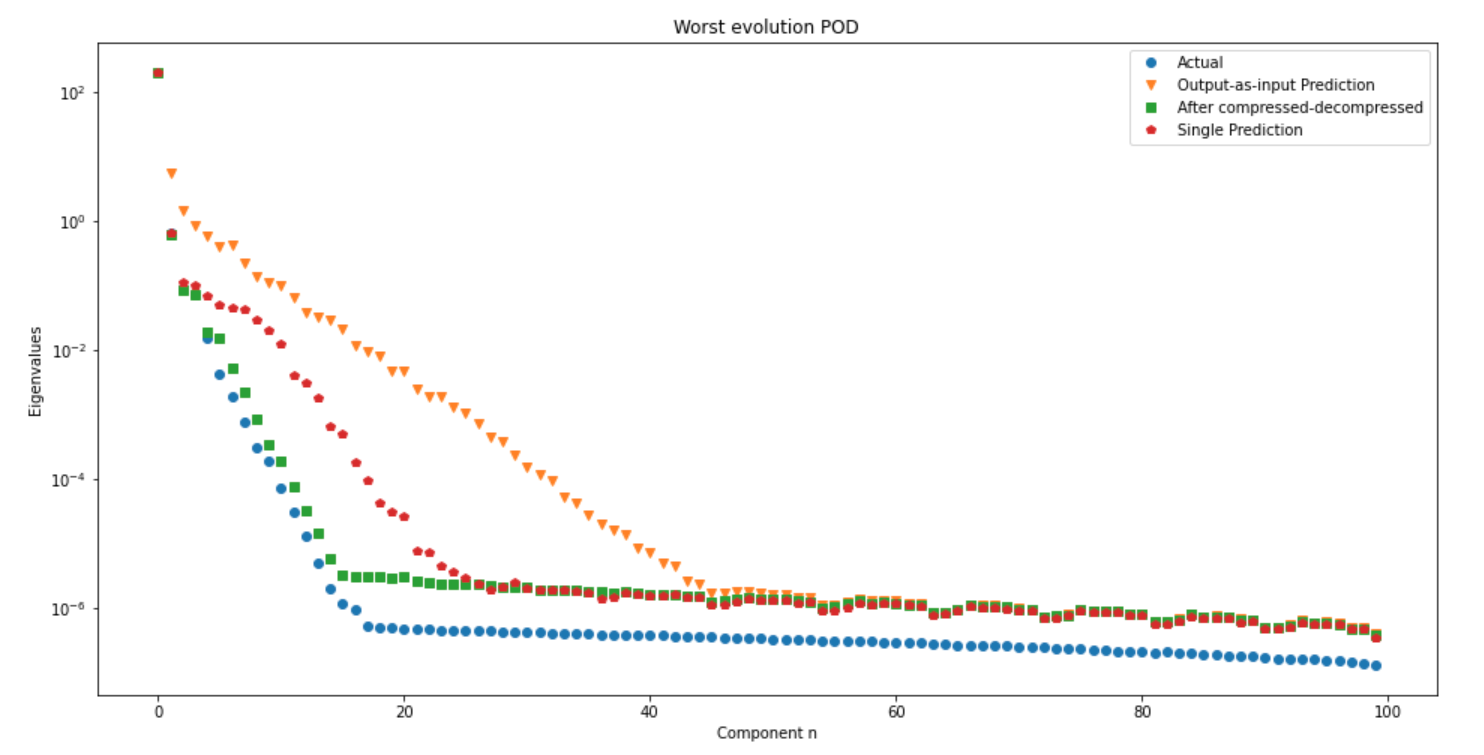
\includegraphics[scale=0.5]{figures/mantle_convection_images/limited_dataset/FNN_Worst_POD.png}
    \label{figure:FNN_limited_worst_POD}
\end{figure}

As seen in the animations and the POD results, the first method (output-as-input prediction) fails to accurately capture the time evolution of the temperature field in the worst case and the prediction is completely different to the actual simulation. This is because the information loss from the ConvAE and FNN in each prediction-as-input loop accumulates, leading to poor results after 99 iterations. In contrast, the prediction result for the second method mostly matches with the actual output in both cases, which is consistent to our hypothesis that the first method itself leads to huge information loss.

Also, the animations of the predicited time-series show that the temperature is being convected either faster or slower than the actual simulation. This is probably due to the varying distance between time steps in the dataset. Under such conditions, the model will try to predict the temperature field at the next time step by averaging out the distance between each time step, thus making the predicted simulations either too fast or too slow.

To explore if we can generate a sequence of temperature fields with less information loss, we try to use LSTM to predict the latent space representation instead. The results are covered in the sequel.


\subsection{Long Short-Term Memory (LSTM) for Prediction}

We now move on to predict a sequence of temperature fields latent space representations using LSTM. The LSTM in this study uses the first 50 temperature fields as a sequence in each file as one training set, takes a sequence of 50 temperature fields as the input, and outputs the remaining 50 temperature fields corresponding to the next time steps.

This 50:50 of input-output length is determined by a PyTorch's technical limitation with LSTMs. In particular, the input length and the output length have to match for the LSTM to functionally work. A ratio of less input length and more output length (20:80) had been considered, but this requires the input sequence to be replicated into 4 times the size to match with PyTorch's constraint, which could lead to worse prediction result compared with the 50:50 ratio.

Therefore, the files in the dataset are randomly shuffled and divided in a ratio of 80\%, 10\%, 10\% for training, testing and validation where each piece of data is a complete file to be divided in half as input and output.

Again, before a sequence of latent space representation is fed as the input to LSTM, it is flattened into a two dimensional array of size $50 \times 6210$. The prediction of LSTM in this case is then resized from $50 \times 6210$ to $50 \times 6 \times 23 \times 45$ for the convenience of further evaluation.

The trainable parameters of LSTM are optimized using small mini-batches (only 1 batch in this case since we have merely 80 training samples) and Adam as the optimizer, where the loss function is defined as the MSE between the prediction of the LSTM and the actual output (both in the shape of a sequence of latent space representation, which is $50 \times 6 \times 23 \times 45$).

After testing several LSTMs with different configurations, we found that architectures with a total number of 2 consecutive LSTM layers perform the best. We also tested some deeper architectures with 4-6 LSTMs. However, there was no significant reduction in the loss value.

In the following figures, we present results from an architecture with 2 LSTM layers (first one input size is 6210, hidden size is 3105; second one input size is 3105, hidden size is 6210. Both of them only have one layer, no internal stacking), and trained for 200 epochs. The results include the training and validation losses in Figure \ref{figure:LSTM_limited_losses}, overall testing result in Figure \ref{figure:LSTM_limited_testing}, and the most/least accurate prediction in Figures \ref{figure:LSTM_limited_best} and \ref{figure:LSTM_limited_worst}, respectively.

\begin{figure}[H]
    \caption{Training and validation losses of LSTM trained with Limited Dataset.}
    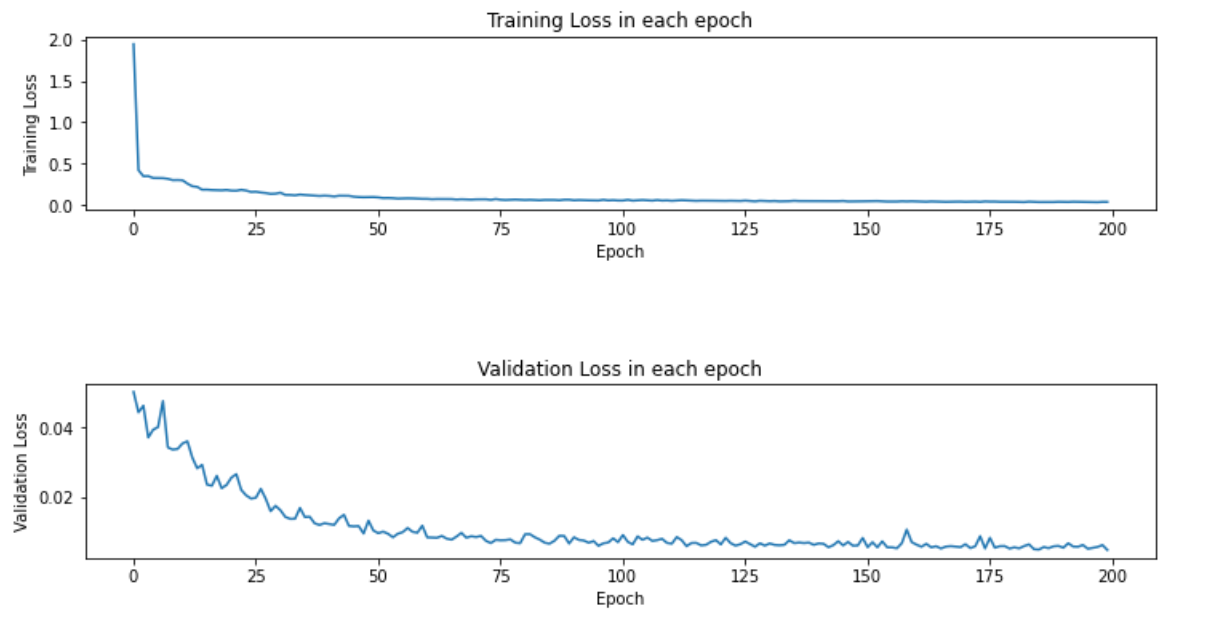
\includegraphics[scale=0.6]{figures/mantle_convection_images/limited_dataset/LSTM_trainingData.png}
    \label{figure:LSTM_limited_losses}
\end{figure}

\begin{figure}[H]
    \caption{Overall testing result of LSTM trained with Limited Dataset.}
    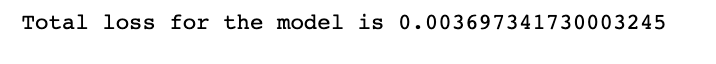
\includegraphics[scale=0.8]{figures/mantle_convection_images/limited_dataset/LSTM_OverallTesting.png}
    \label{figure:LSTM_limited_testing}
\end{figure}

\begin{figure}[H]
    \caption{Ground truth, ground truth after ConvAE's compression-decompression, and most accurate prediction of LSTM trained with Limited Dataset.}
    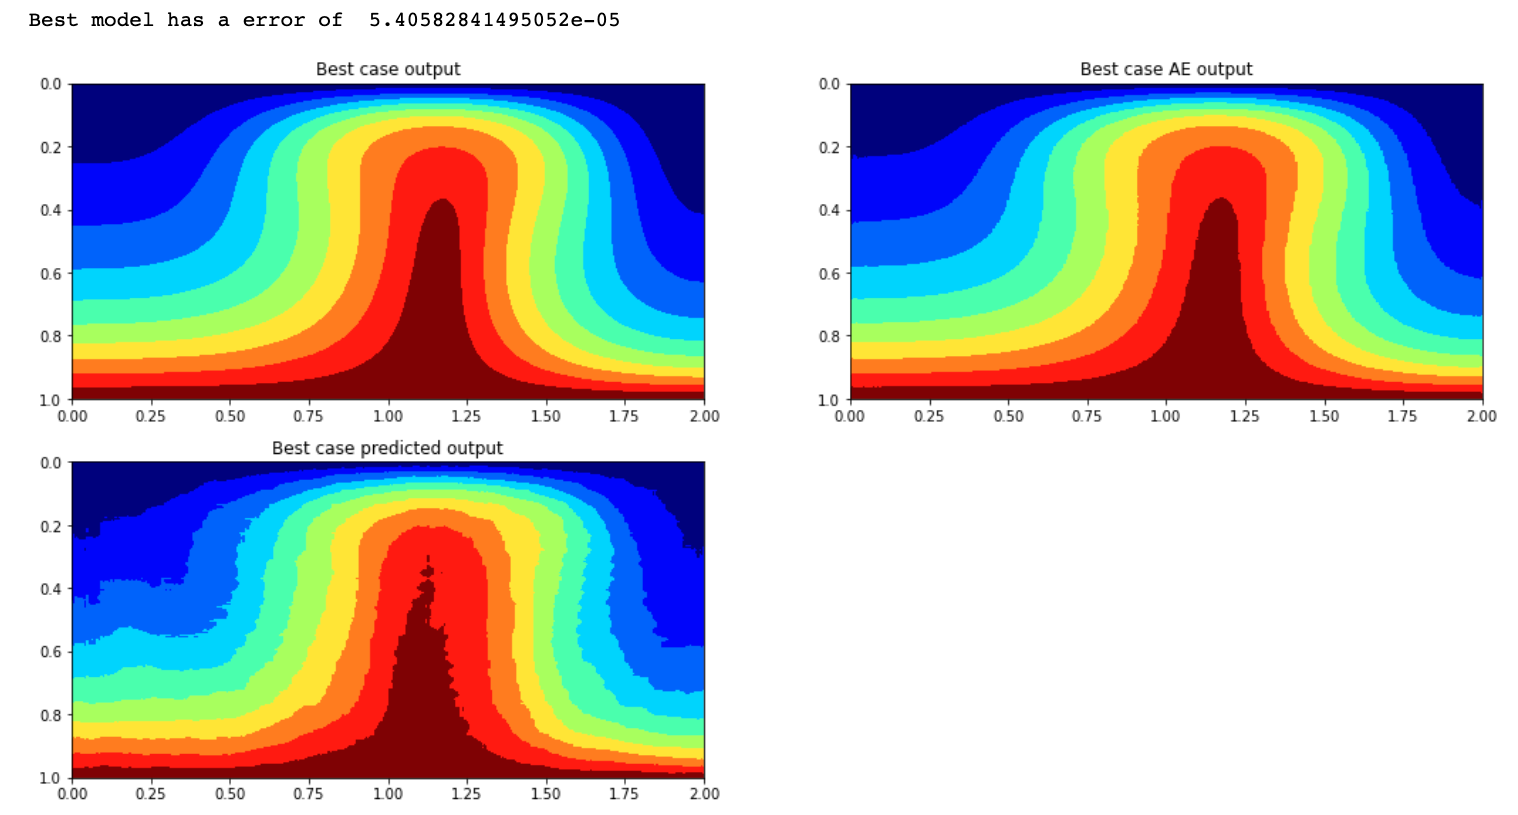
\includegraphics[scale=0.5]{figures/mantle_convection_images/limited_dataset/LSTM_Best.png}
    \label{figure:LSTM_limited_best}
\end{figure}

\begin{figure}[H]
    \caption{Ground truth, ground truth after ConvAE's compression-decompression, and least accurate prediction of LSTM trained with Limited Dataset.}
    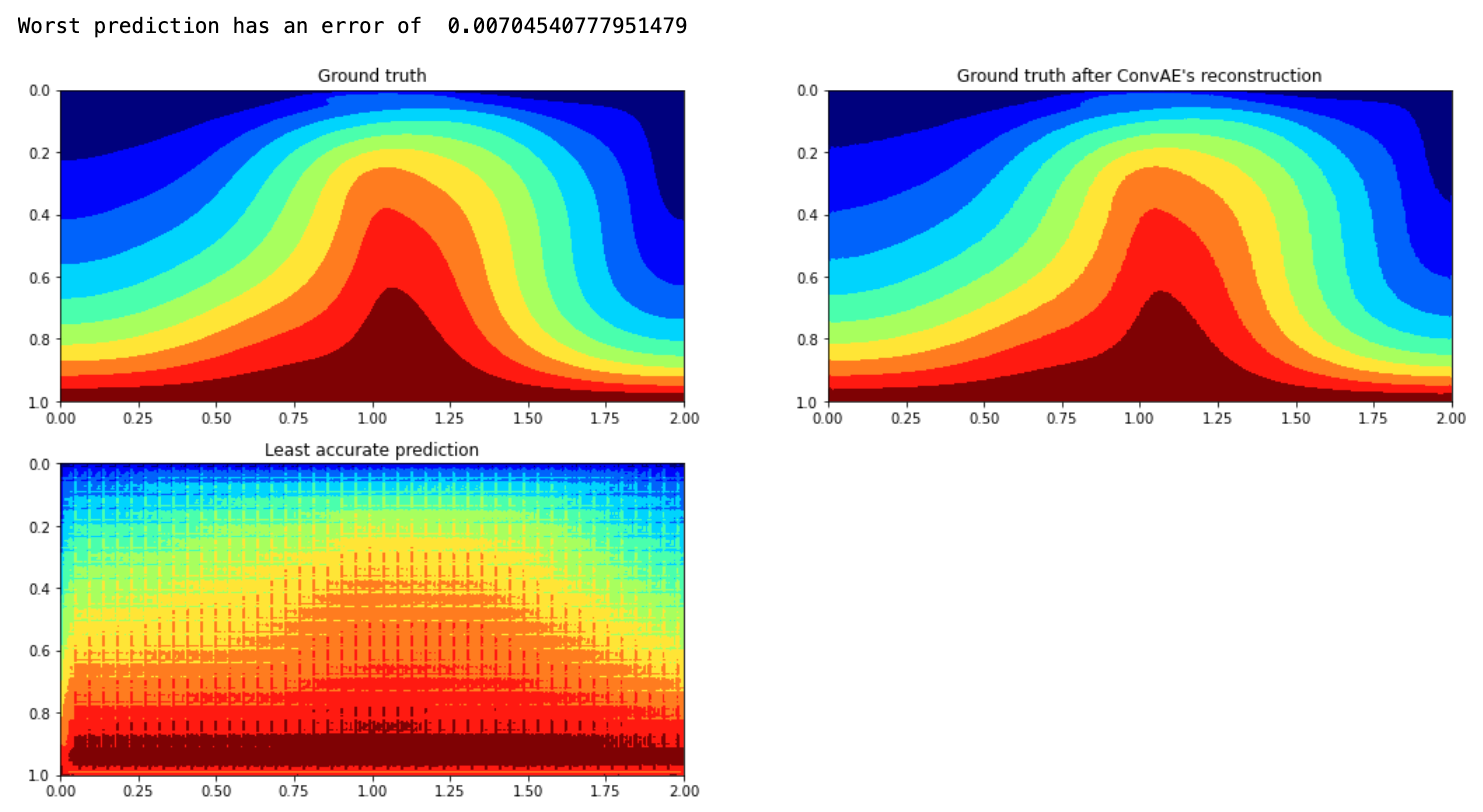
\includegraphics[scale=0.5]{figures/mantle_convection_images/limited_dataset/LSTM_Worst.png}
    \label{figure:LSTM_limited_worst}
\end{figure}

On average, the loss values are higher than the FNN and no overfitting occurs. The prediction is able to capture the main features precisely with some small information loss in the best case, but fails to do so in the worst case. This is caused by the internal structure of LSTM since the worst case is the first temperature field in the output sequence.

To better visualize the prediction result of LSTM on a 50:50 input length to output length ratio, two animations representing the best and worst cases (evaluated based on the sum of MSE for each predicted temperature in the output sequence) in the format of animated files are generated. From top to bottom, the first picture represents the actual output from the dataset and the second one represents the prediction result.

Figure \ref{figure:LSTM_limited_best_gif} and Figure \ref{figure:LSTM_limited_worst_gif} show 20\% of the two sprite sheets converted from the original animation files (every 5th frame) for reading convenience.

\begin{figure}[H]
    \centering
    \caption{Best case animation sheet of LSTM trained with Limited Dataset (Link to animation: \url{https://drive.google.com/file/d/1zNJrZUB8XBAEWsUHPd2NANuWkE8yNg3z/view?usp=sharing})}
    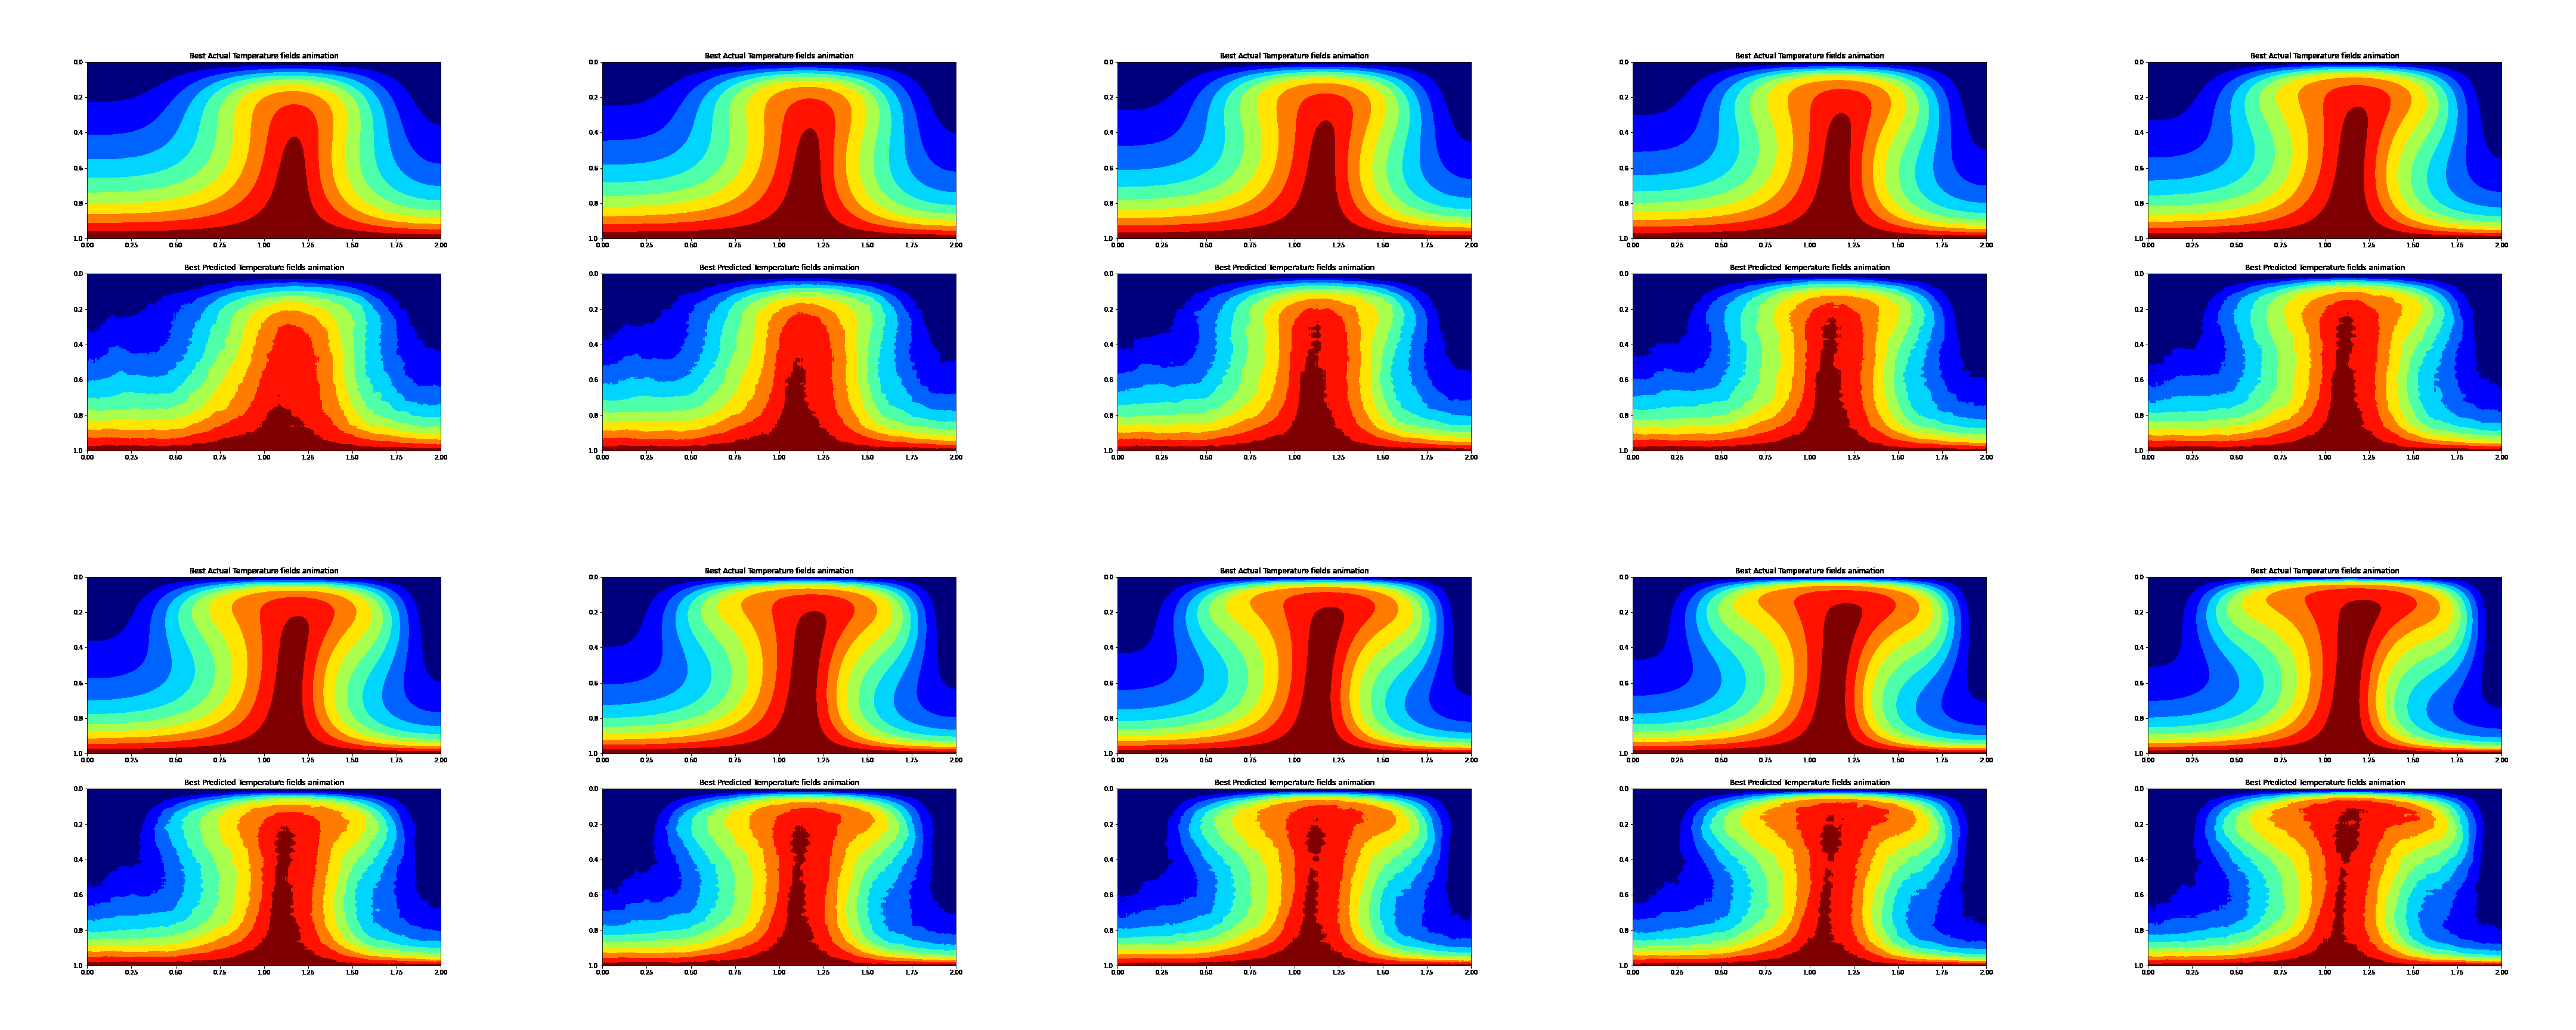
\includegraphics[scale=0.10]{figures/mantle_convection_images/limited_dataset/LSTM_Best_GIF_sheet.png}
    \label{figure:LSTM_limited_best_gif}
\end{figure}



\begin{figure}[H]
    \centering
    \caption{Worst case animation sheet of LSTM trained with Limited Dataset (Link to animation: 
    \url{https://drive.google.com/file/d/1nINRk2Oh8rgQBLWio_b6R6I7T18e7Zi-/view?usp=sharing})}
    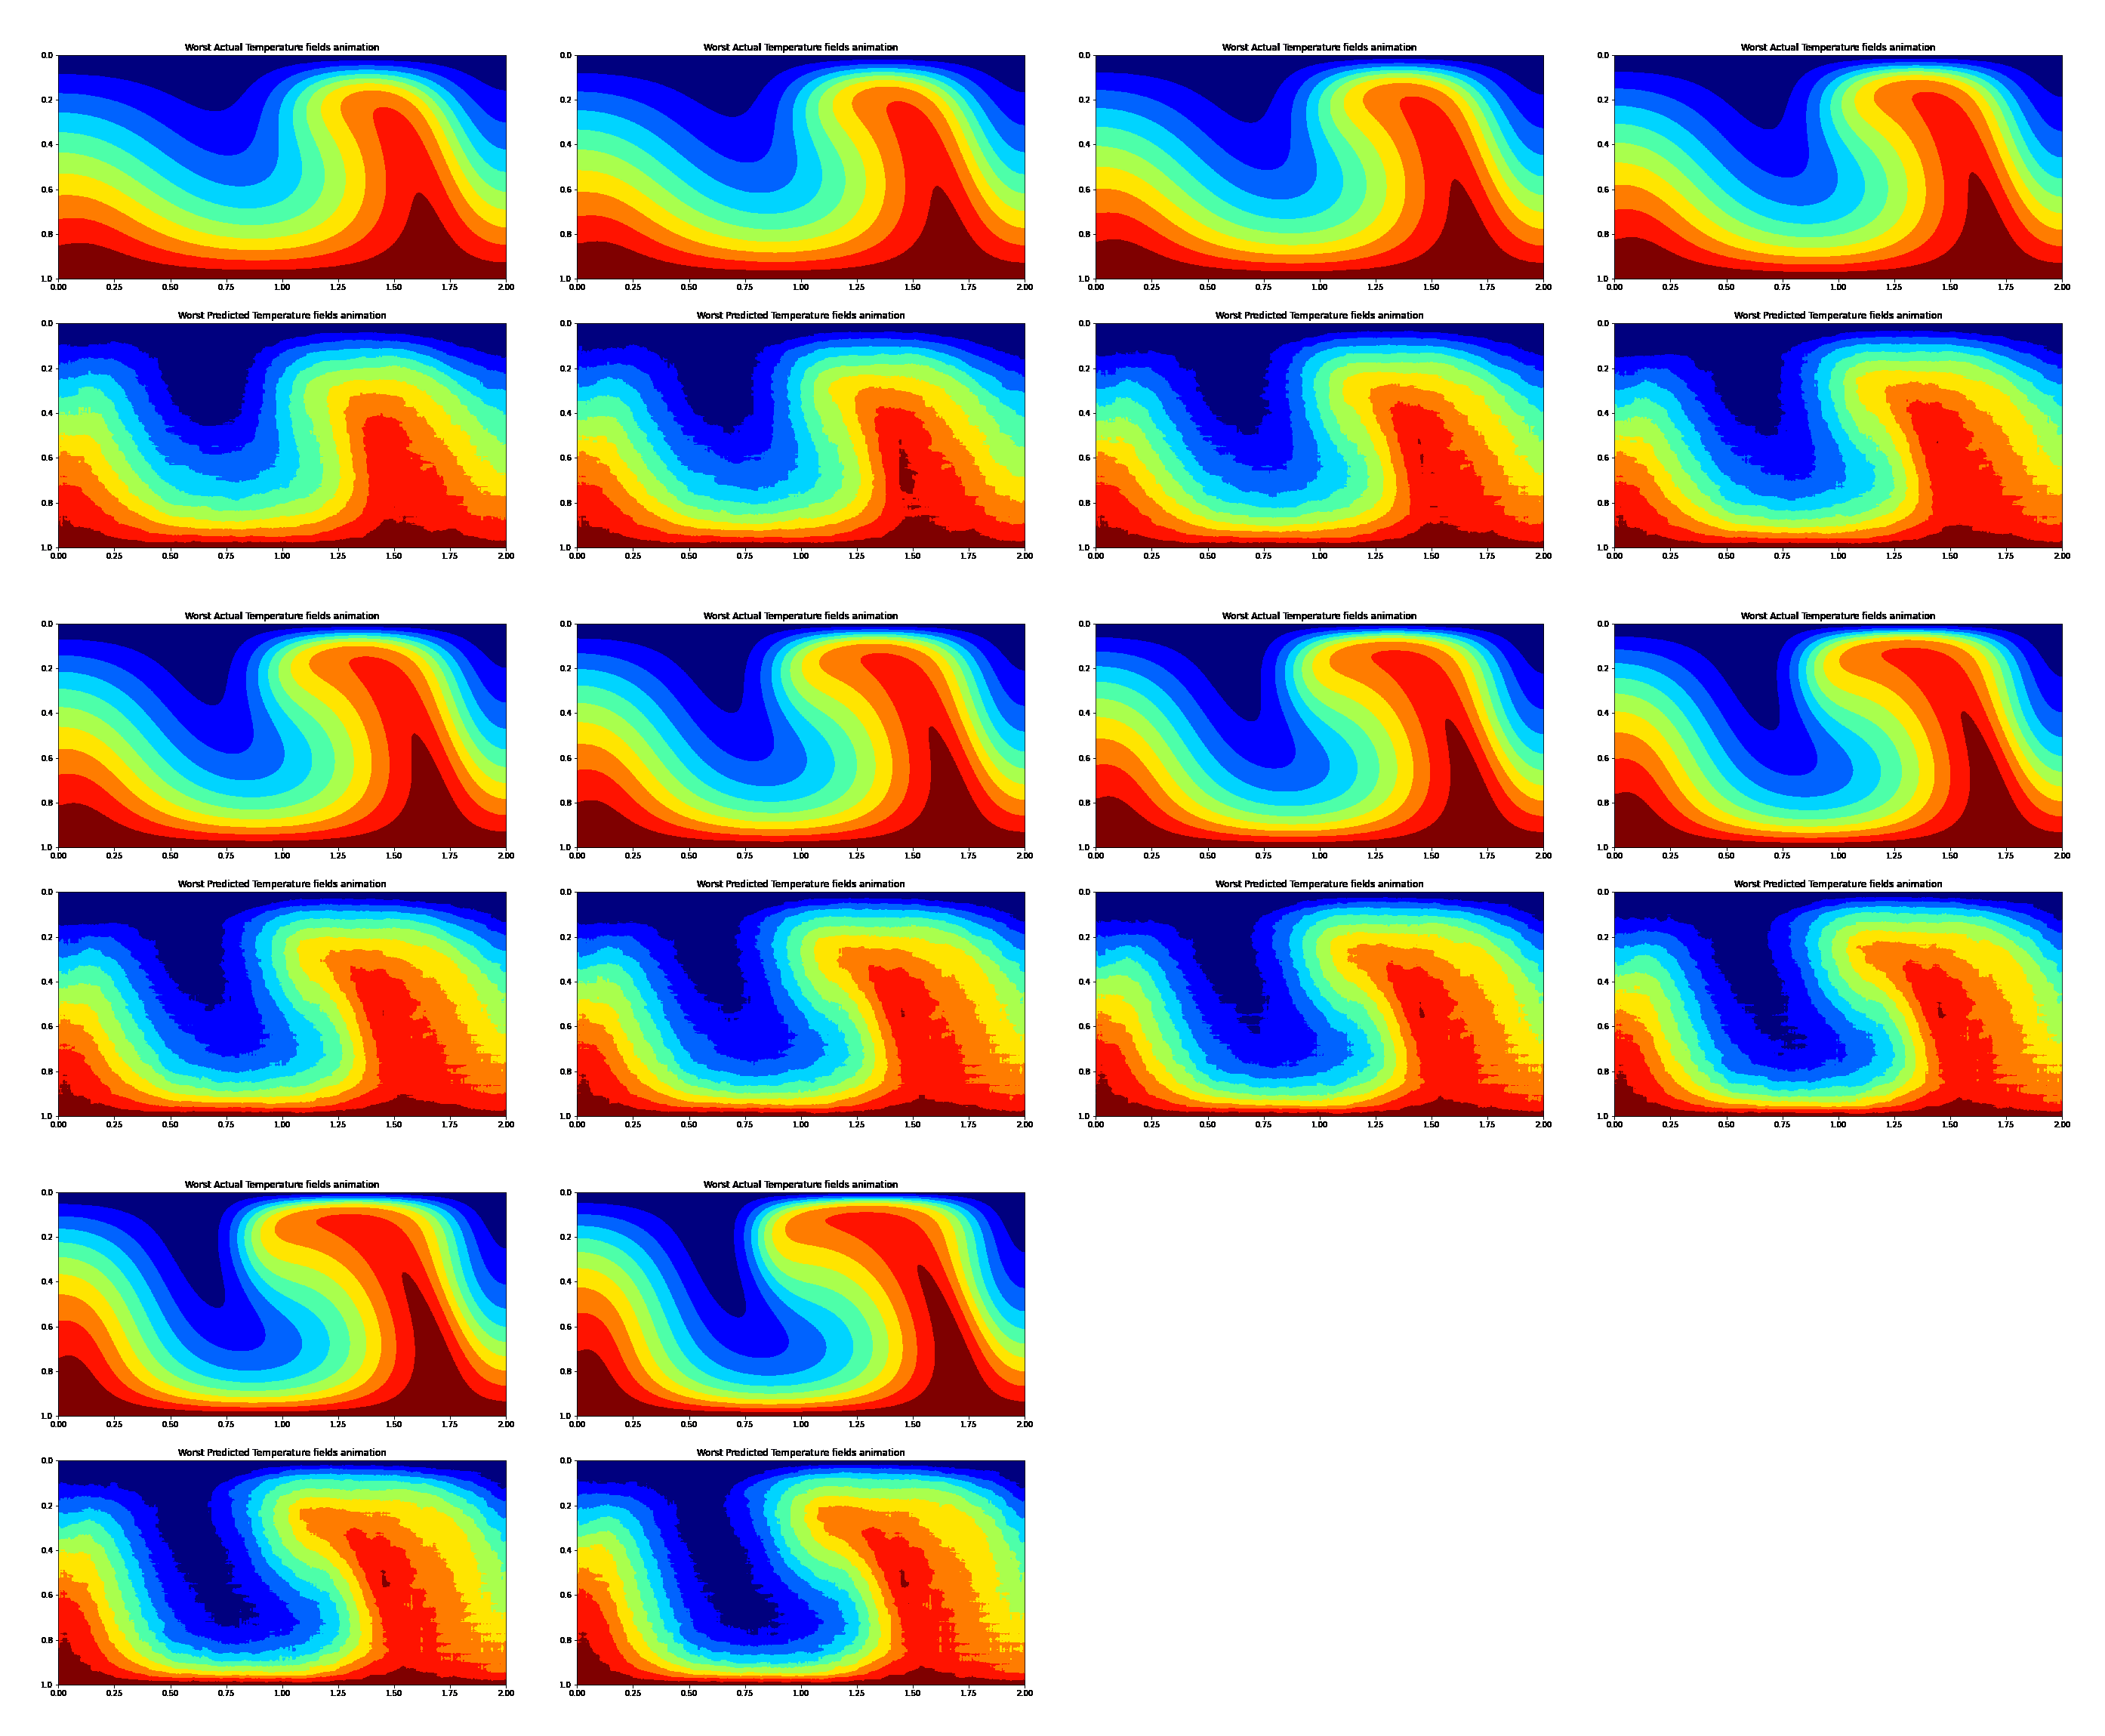
\includegraphics[scale=0.10]{figures/mantle_convection_images/limited_dataset/LSTM_Worst_GIF_sheet.png}
    \label{figure:LSTM_limited_worst_gif}
\end{figure}

To further evaluate the performance, we also applied POD to a sequence of predictions generated by LSTM in both the best and worst cases. As with the FNN, we also consider as a contrast the POD of the original time series and the compressed-decompressed version generated by ConvAE. Figures \ref{figure:LSTM_limited_best_POD} and \ref{figure:LSTM_limited_worst_POD} show the POD results in the best and  worst cases, respectively.

\begin{figure}[H]
    \caption{Best case POD of LSTM trained with Limited Dataset.}
    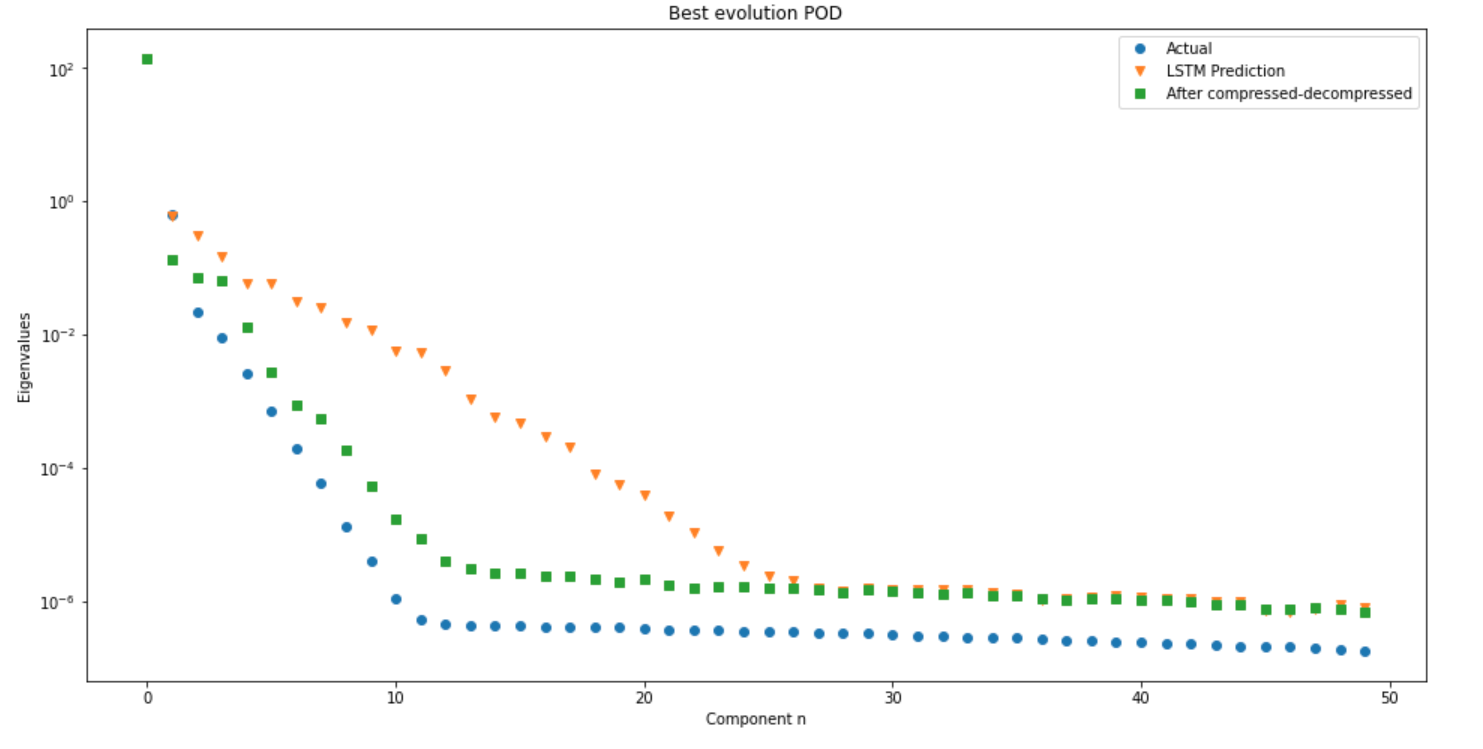
\includegraphics[scale=0.5]{figures/mantle_convection_images/limited_dataset/LSTM_Best_POD.png}
    \label{figure:LSTM_limited_best_POD}
\end{figure}

\begin{figure}[H]
    \caption{Worst case POD of LSTM trained with Limited Dataset.}
    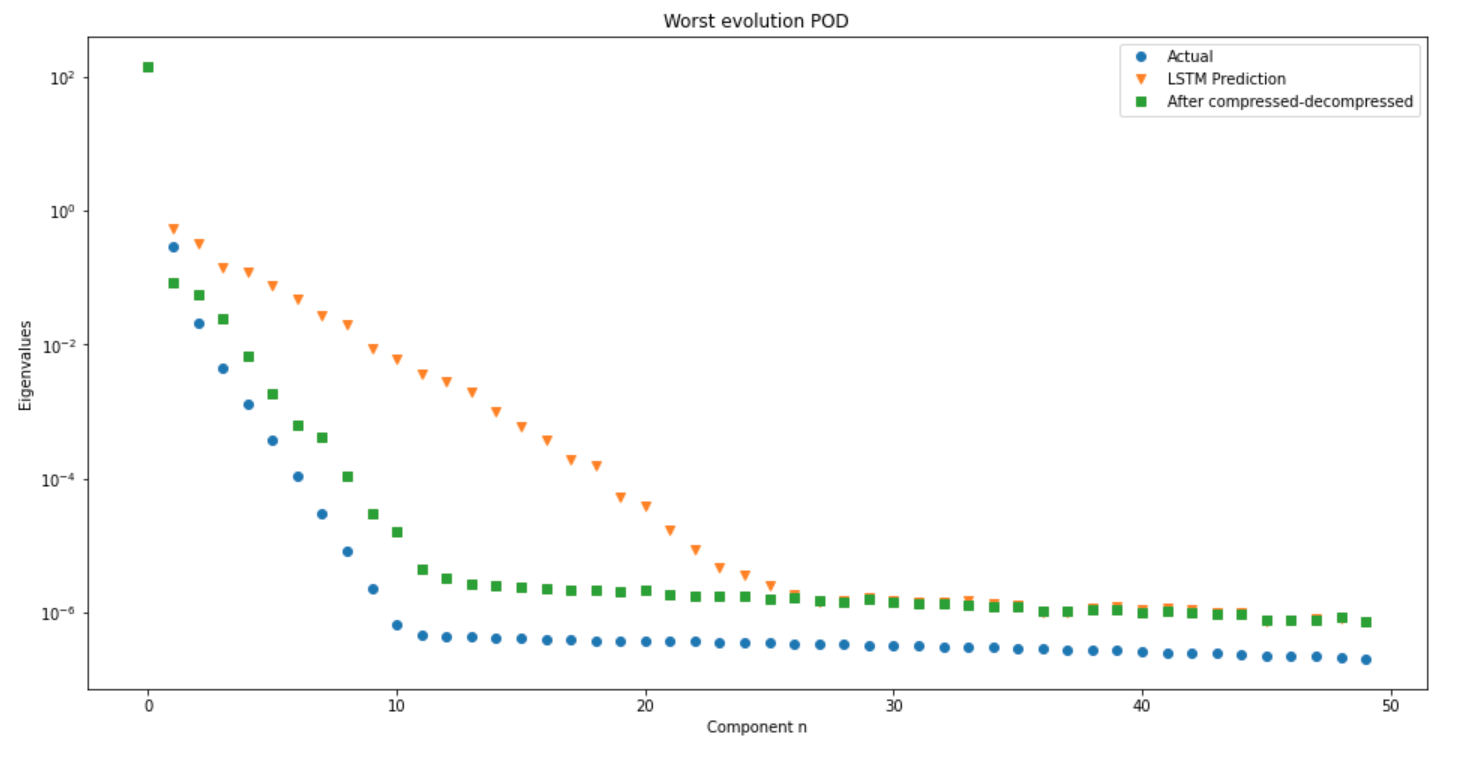
\includegraphics[scale=0.5]{figures/mantle_convection_images/limited_dataset/LSTM_Worst_POD.png}
    \label{figure:LSTM_limited_worst_POD}
\end{figure}

From the animations and the POD results, we can conclude that LSTM is able to better capture the dynamics of the simulations even in its worst case. However, the simulations predicted using LSTM are less accurate and have more data loss compared with those predicted using FNN. There could be potential underfitting problem due to the lack of training data since only 80 samples are used for training.


\section{Mantle Convection Simulation on Larger Dataset}

To confirm if the low accuracy of LSTM is caused by the scarceness of data, a larger dataset is tested, whose only two differences with the limited dataset are that it now contains 903 simulations and it uses absolute time steps instead of adaptive time steps. However, even though it now uses absolute time steps, the distance between each of the consecutive time steps still varies.

For this section, the distance between time steps are not considered since we want to mainly focus on testing if the scarceness of data is the reason for the low accuracy of LSTM. Nevertheless, time steps will be used in the next section to create an interpolated dataset.

The larger dataset are randomly divided in the same way as the limited dataset for each of the three ML architectures in the following subsections.

\subsection{Compression of temperature fields}

The ConvAE used for compressing the temperature fields in this section has the same structure and hyperparameters values as the one trained with limited dataset, except for the total number of epochs, which are now reduced from 1,000 to 200 due to the computational budget limitations on Gadi.

In the following figures, some detailed test results from this ConvAE trained with the larger dataset are presented, including the training and validation losses in Figure \ref{figure:ConvAE_larger_losses}, overall testing result in Figure \ref{figure:ConvAE_larger_testing}, and the most/least accurate prediction in Figure \ref{figure:ConvAE_larger_best_worst}.

\begin{figure}[H]
    \caption{Training and validation losses of ConvAE trained with Larger Dataset.}
    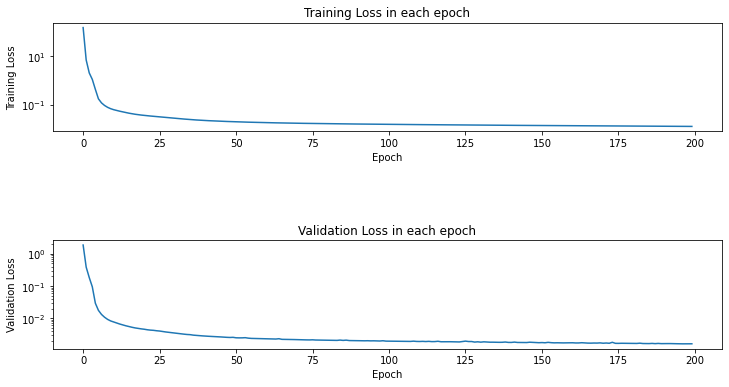
\includegraphics[scale=0.6]{figures/mantle_convection_images/larger_dataset/ConvAE_trainingData.png}
    \label{figure:ConvAE_larger_losses}
\end{figure}

\begin{figure}[H]
    \caption{Overall testing result of ConvAE trained with Larger Dataset.}
    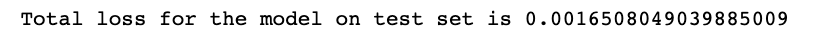
\includegraphics[scale=0.8]{figures/mantle_convection_images/larger_dataset/ConvAE_OverallTesting.png}
    \label{figure:ConvAE_larger_testing}
\end{figure}

\begin{figure}[H]
\centering
\begin{subfigure}{0.45\textwidth}
    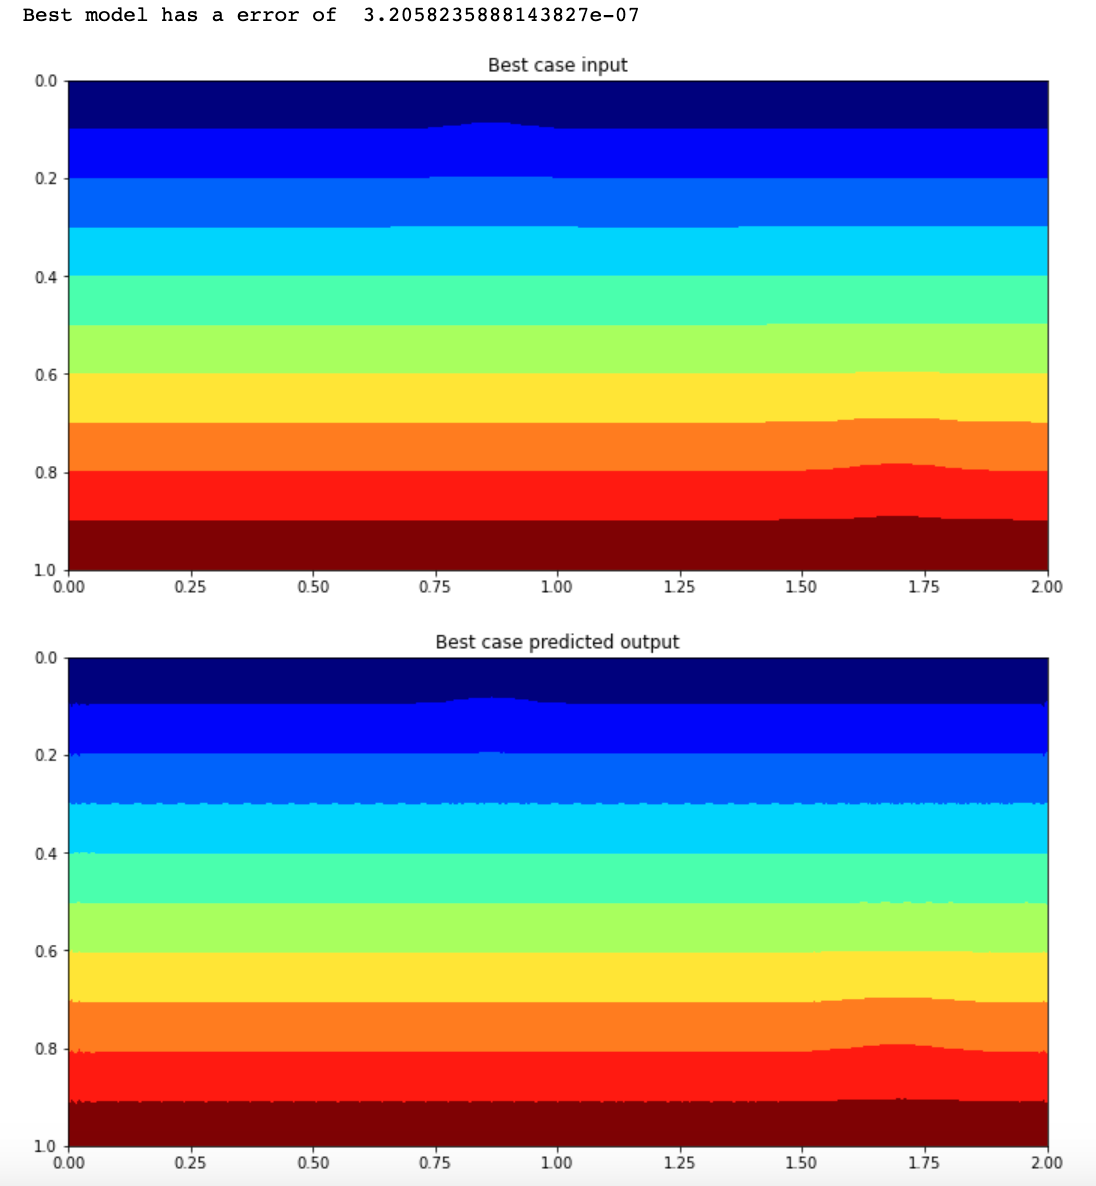
\includegraphics[width=\textwidth]{figures/mantle_convection_images/larger_dataset/ConvAE_Best.png}
    \caption{Most accurate reconstruction of ConvAE trained with Larger Dataset.}
\end{subfigure}
\hfill
\begin{subfigure}{0.45\textwidth}
    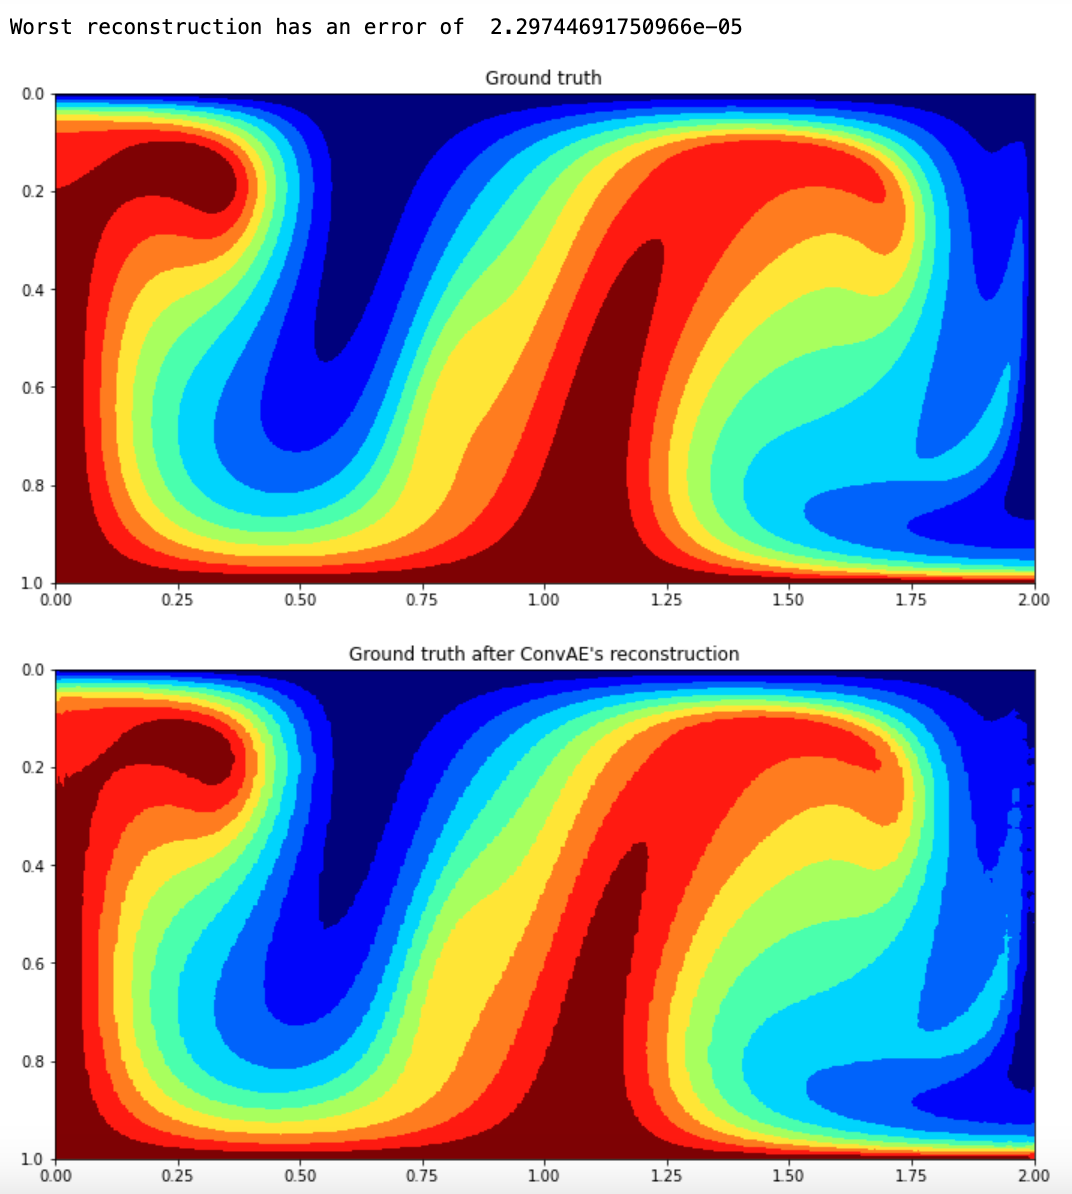
\includegraphics[width=\textwidth]{figures/mantle_convection_images/larger_dataset/ConvAE_Worst.png}
    \caption{Least accurate reconstruction of ConvAE trained with Larger Dataset.}
\end{subfigure}   
\caption{Best case and worst case using ConvAE.}
\label{figure:ConvAE_larger_best_worst}
\end{figure}

Overall, the performance of this ConvAE is similar to the one trained with the limited dataset: reconstruction loss is low and no overfitting occurs.


\subsection{Fully Connected Neural Network for Prediction}

The FNN in this section also has the same structure and the same set of hyperparameters as the one trained with the limited dataset, except that the total number of epochs is reduced from 1,000 to 200 as well.

The results are presented in the following figures, including the training and validation losses from Figure \ref{figure:FNN_larger_losses}, overall testing result from Figure \ref{figure:FNN_larger_testing}, and the most/least accurate prediction in Figures \ref{figure:FNN_larger_best} and \ref{figure:FNN_larger_worst}, respectively.

\begin{figure}[H]
    \caption{Training and validation losses of FNN trained with Larger Dataset.}
    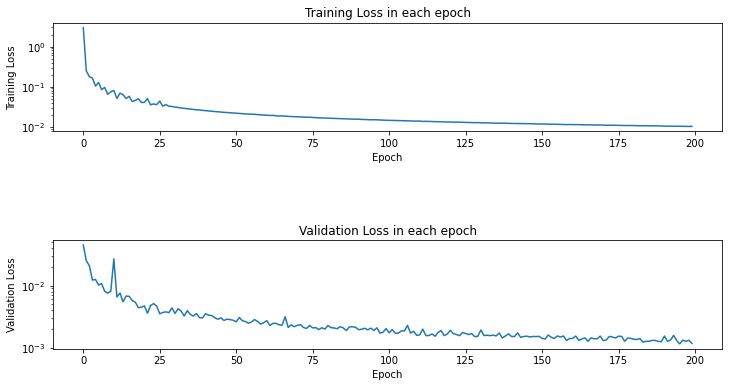
\includegraphics[scale=0.6]{figures/mantle_convection_images/larger_dataset/FNN_trainingData.png}
    \label{figure:FNN_larger_losses}
\end{figure}

\begin{figure}[H]
    \caption{Overall testing result of FNN trained with Larger Dataset.}
    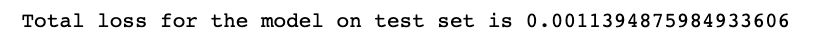
\includegraphics[scale=0.8]{figures/mantle_convection_images/larger_dataset/FNN_OverallTesting.png}
    \label{figure:FNN_larger_testing}
\end{figure}

\begin{figure}[H]
    \caption{Ground truth, ground truth after ConvAE's compression-decompression, and most accurate prediction of FNN trained with Larger Dataset.}
    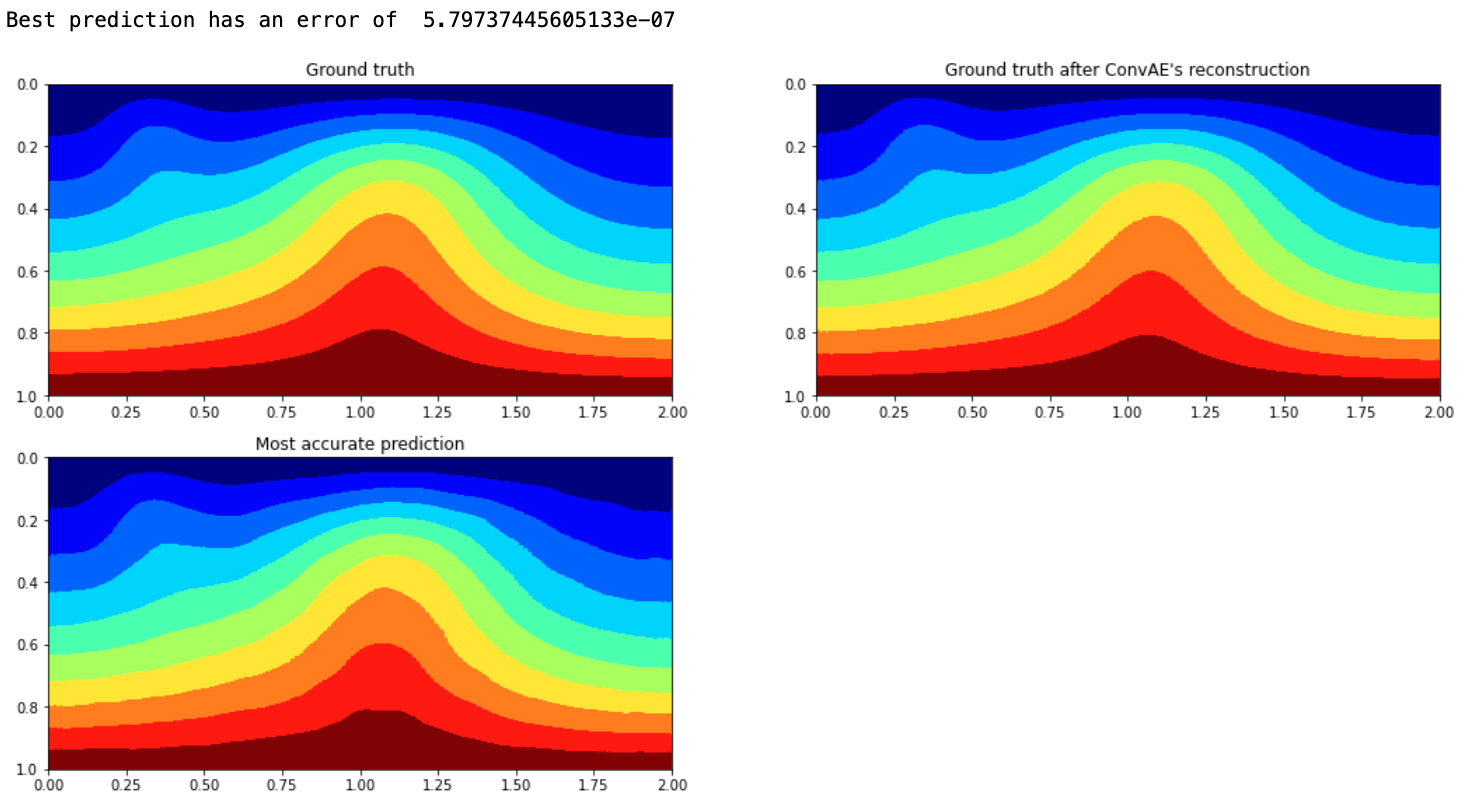
\includegraphics[scale=0.5]{figures/mantle_convection_images/larger_dataset/FNN_Best.png}
    \label{figure:FNN_larger_best}
\end{figure}

\begin{figure}[H]
    \caption{Ground truth, ground truth after ConvAE's compression-decompression, and least accurate prediction of FNN trained with Larger Dataset.}
    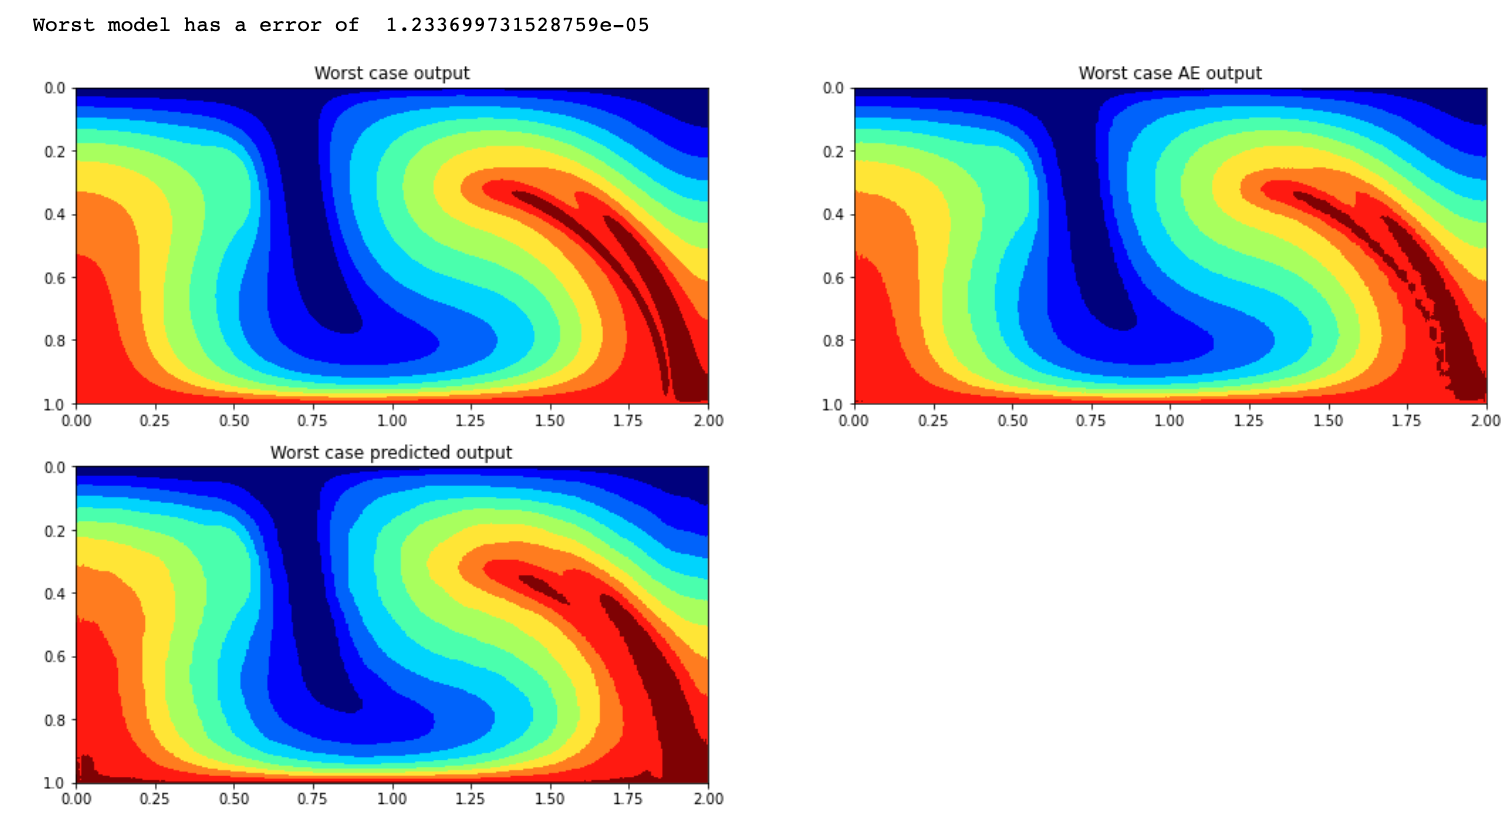
\includegraphics[scale=0.5]{figures/mantle_convection_images/larger_dataset/FNN_Worst.png}
    \label{figure:FNN_larger_worst}
\end{figure}

The results obtained with the FNN are similar to the ones obtained with the limited dataset: loss values are low and no overfitting occurs. There is still some small information loss, which is now confirmed as caused by the loss of data generated during the compression-decompression process of ConvAE.

Again, two animations representing the best and worst cases when predicting the entire simulation using "One-for-All" (use $T1$ from dataset $\rightarrow$ get predicted $T2$ $\rightarrow$ use predicted $T2$ $\rightarrow$ get predicted $T3$ $\rightarrow$ ...) are generated.

Figures \ref{figure:FNN_larger_best_gif} and \ref{figure:FNN_larger_worst_gif} show 10\% of the two sprite sheets converted from the original animation files (Every 10th frame).

\begin{figure}[H]
    \centering
    \caption{Best case animation sheet of FNN trained with Larger Dataset (Link to animation: \url{https://drive.google.com/file/d/1LxuwXxEoG5xsYzLYn6n6-mUfoP8A3IC2/view?usp=sharing})}
    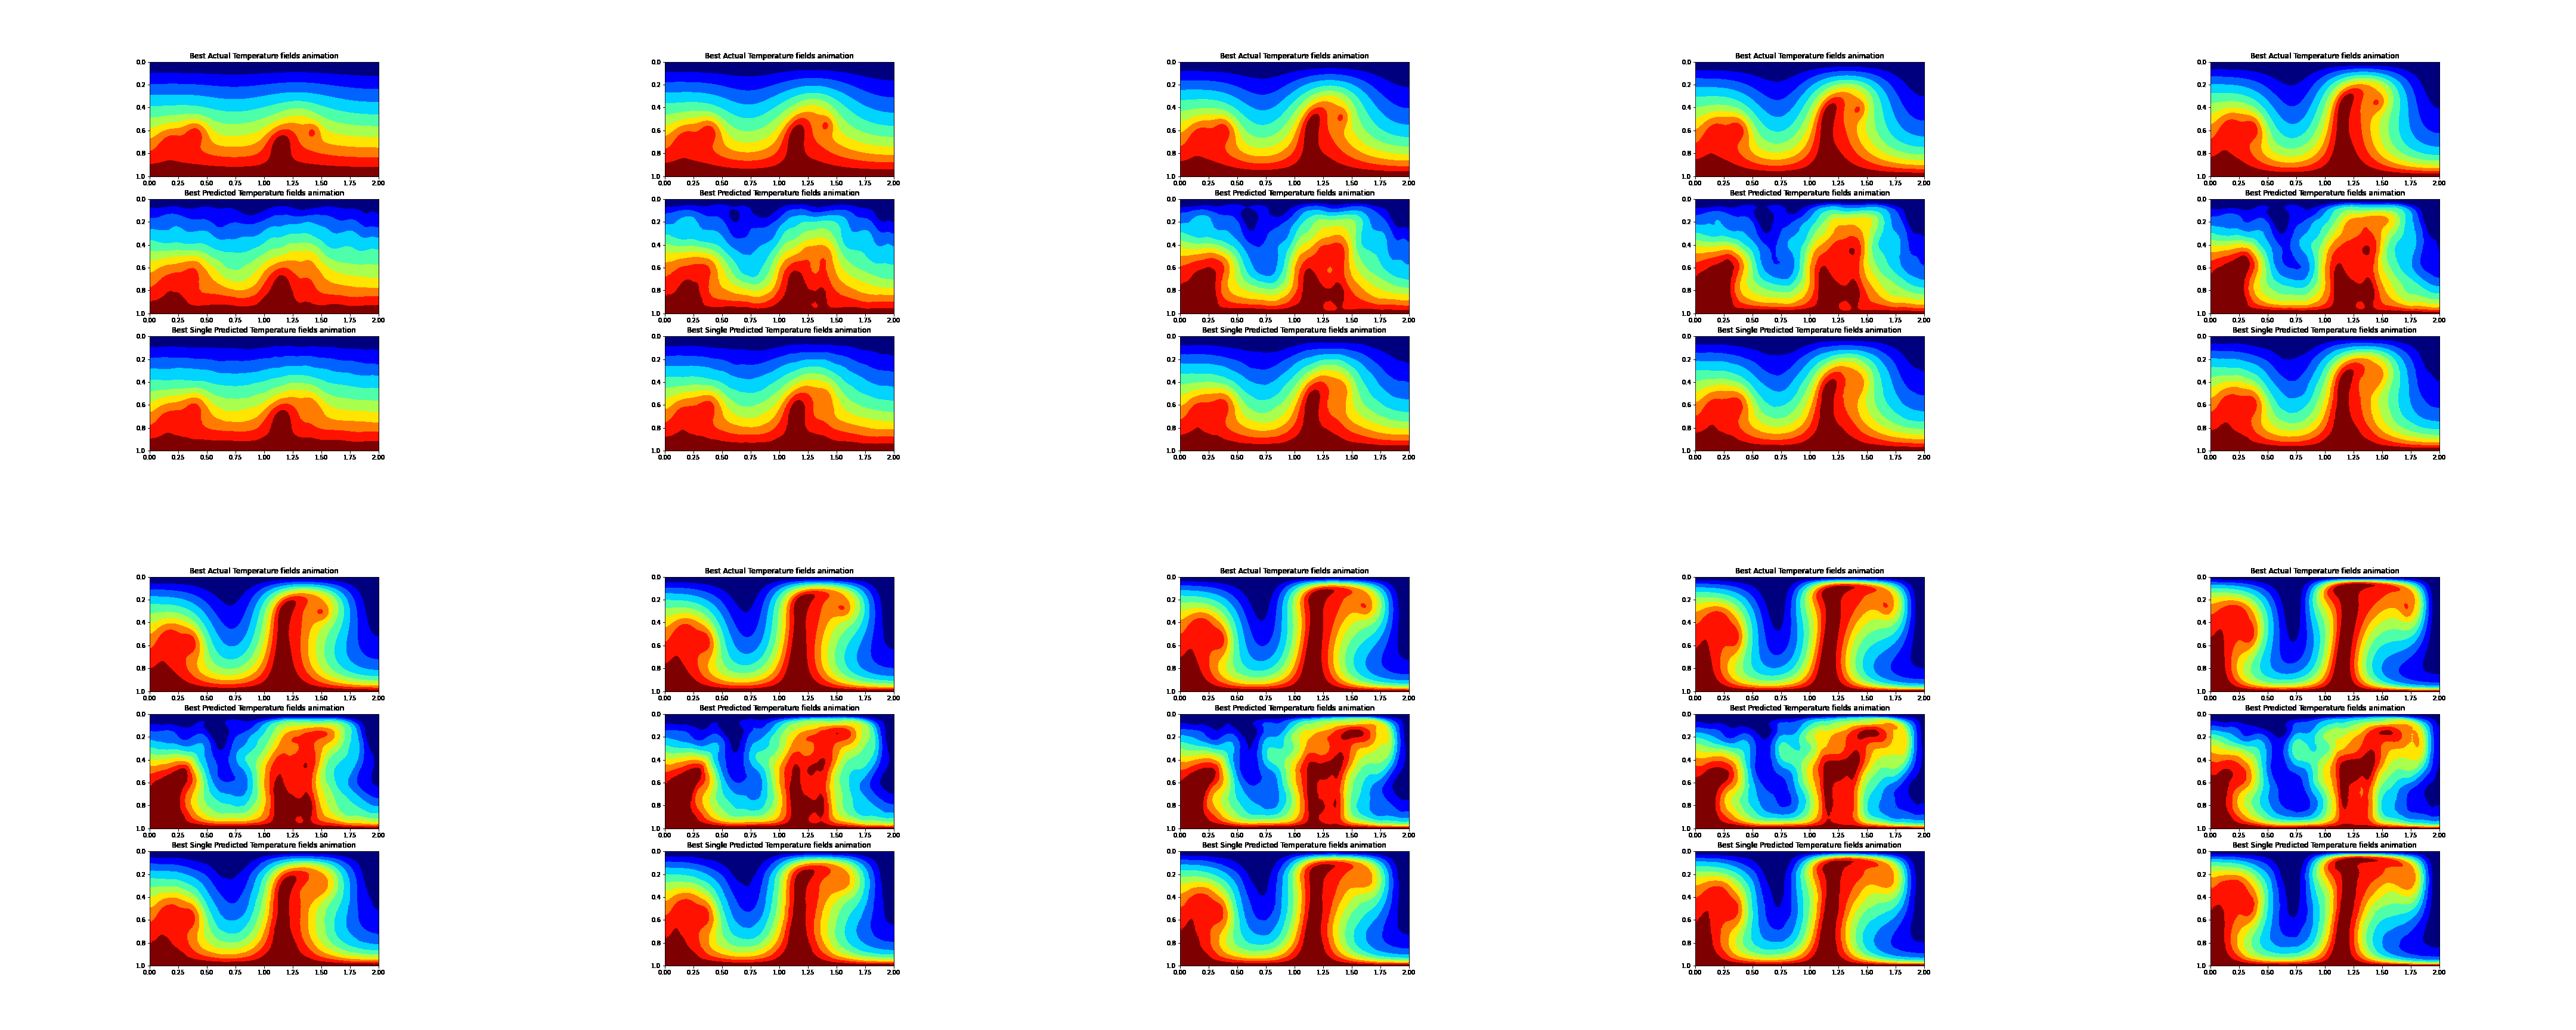
\includegraphics[scale=0.10]{figures/mantle_convection_images/larger_dataset/FNN_Best_GIF_sheet.png}
    \label{figure:FNN_larger_best_gif}
\end{figure}

\begin{figure}[H]
    \centering
    \caption{Worst case animation sheet of FNN trained with Larger Dataset (Link to animation: 
    \url{https://drive.google.com/file/d/1vwfL_n6ANnkJEY3B8a024SF_yQ35Hkxu/view?usp=sharing})}
    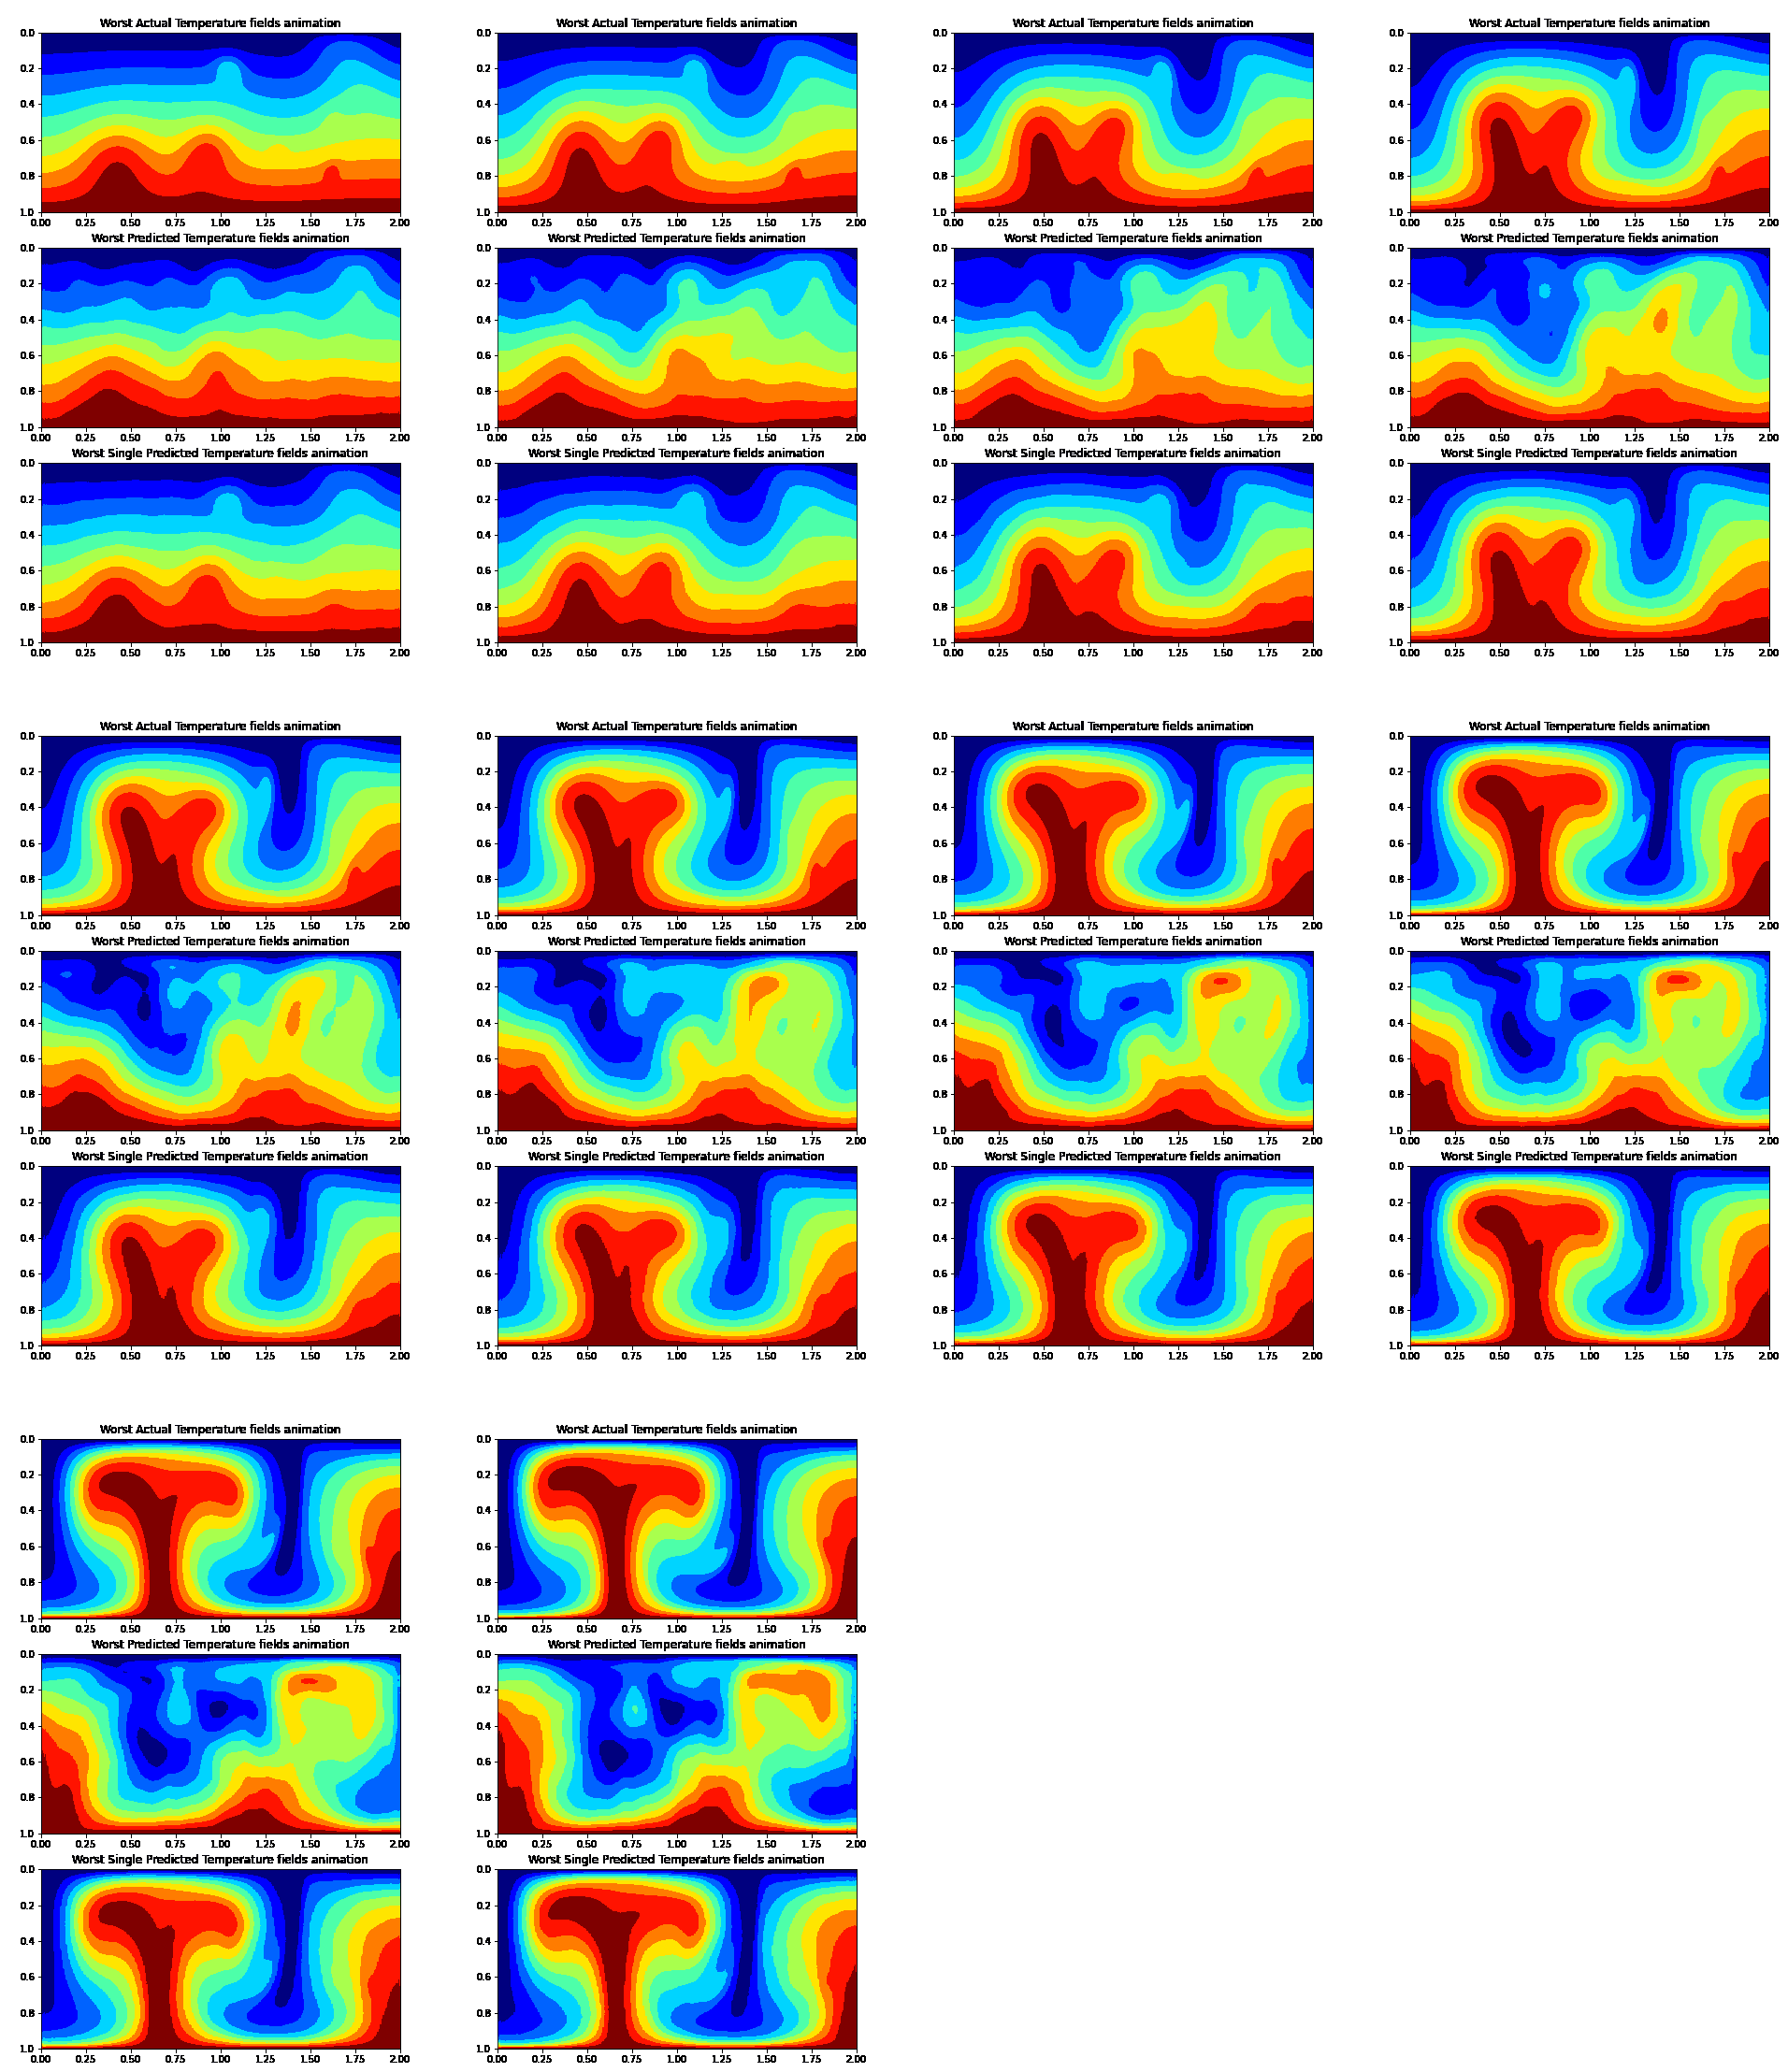
\includegraphics[scale=0.10]{figures/mantle_convection_images/larger_dataset/FNN_Worst_GIF_sheet.png}
    \label{figure:FNN_larger_worst_gif}
\end{figure}

POD results for the best and worst cases are shown in Figures \ref{figure:FNN_larger_best_POD} and \ref{figure:FNN_larger_worst_POD}, respectively.

\begin{figure}[H]
    \caption{Best case POD of FNN trained with Larger Dataset.}
    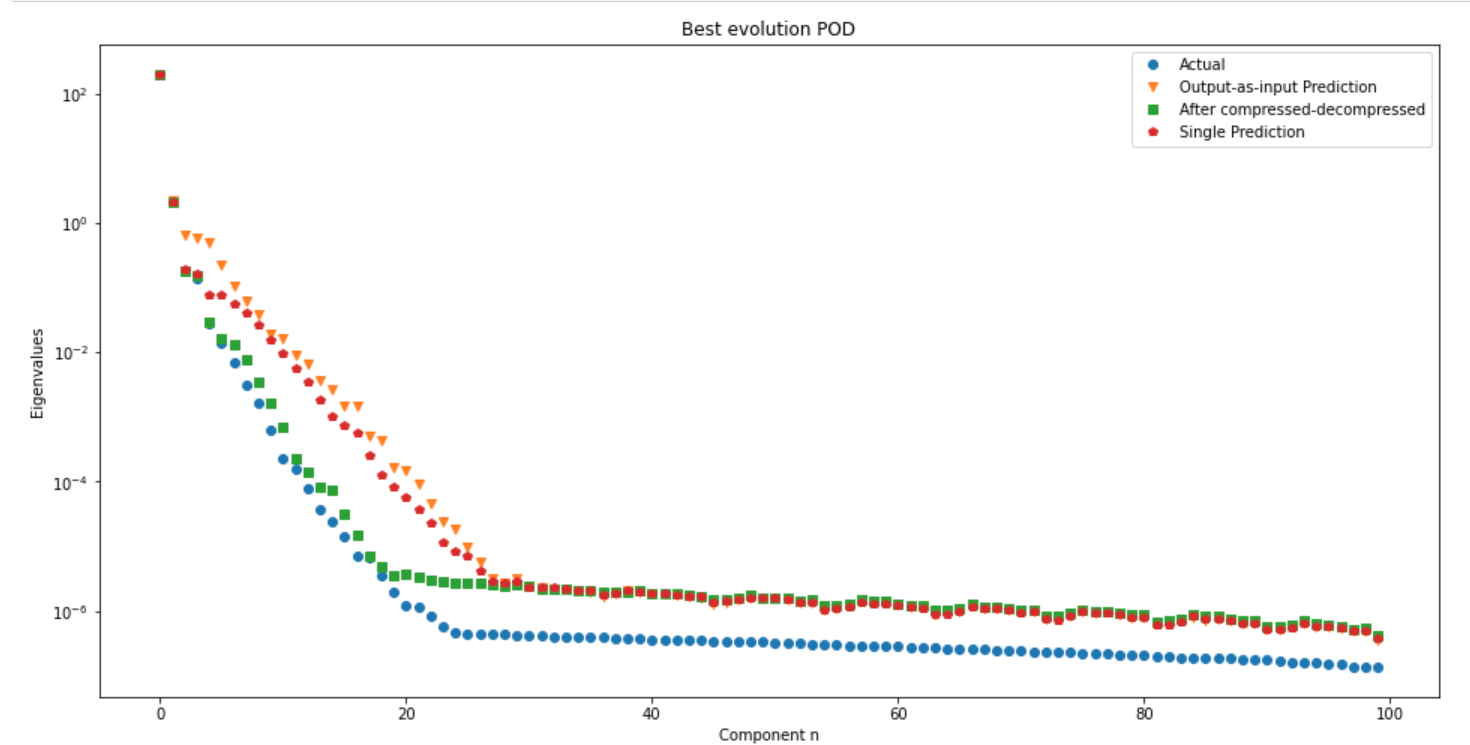
\includegraphics[scale=0.5]{figures/mantle_convection_images/larger_dataset/FNN_Best_POD.png}
    \label{figure:FNN_larger_best_POD}
\end{figure}

\begin{figure}[H]
    \caption{Worst case POD of FNN trained with Larger Dataset.}
    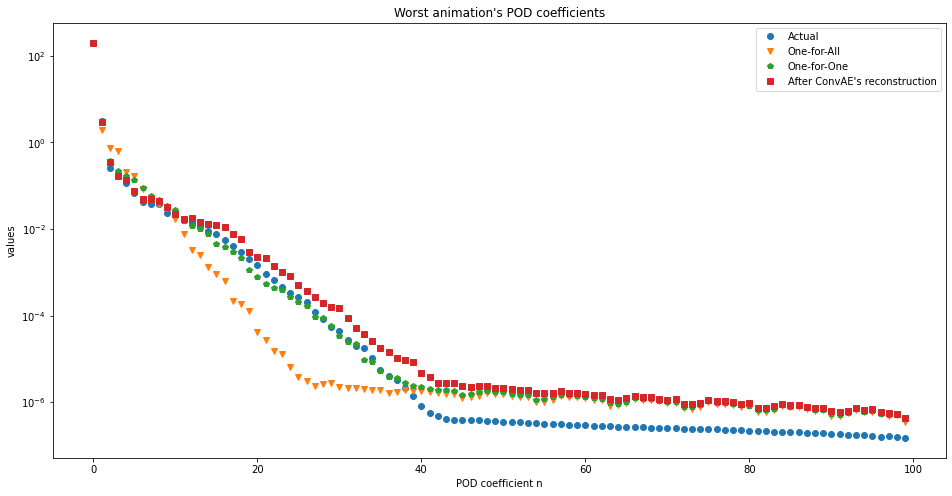
\includegraphics[scale=0.5]{figures/mantle_convection_images/larger_dataset/FNN_Worst_POD.png}
    \label{figure:FNN_larger_worst_POD}
\end{figure}

We can observe that the increasing size of the training data does not improve the quality of the animations when predicting the entire simulations using the first method. Also, apart from the information loss, the problem of the predicted time temperature evolution moving too fast or too slow still exists.


\subsection{Long Short-Term Memory (LSTM) for Prediction}

The LSTM in this section also has the same structure and the same set of hyperparamters as the one trained with limited dataset, except that the total number of epochs are reduced from 200 to 100.

The results are presented in the following figures, including the training and validation losses from Figure \ref{figure:LSTM_larger_losses}, overall testing result from Figure \ref{figure:LSTM_larger_testing}, and the most/least accurate prediction in Figures \ref{figure:LSTM_larger_best} and \ref{figure:LSTM_larger_worst}, respectively.

\begin{figure}[H]
    \caption{Training and validation losses of LSTM trained with Larger Dataset.}
    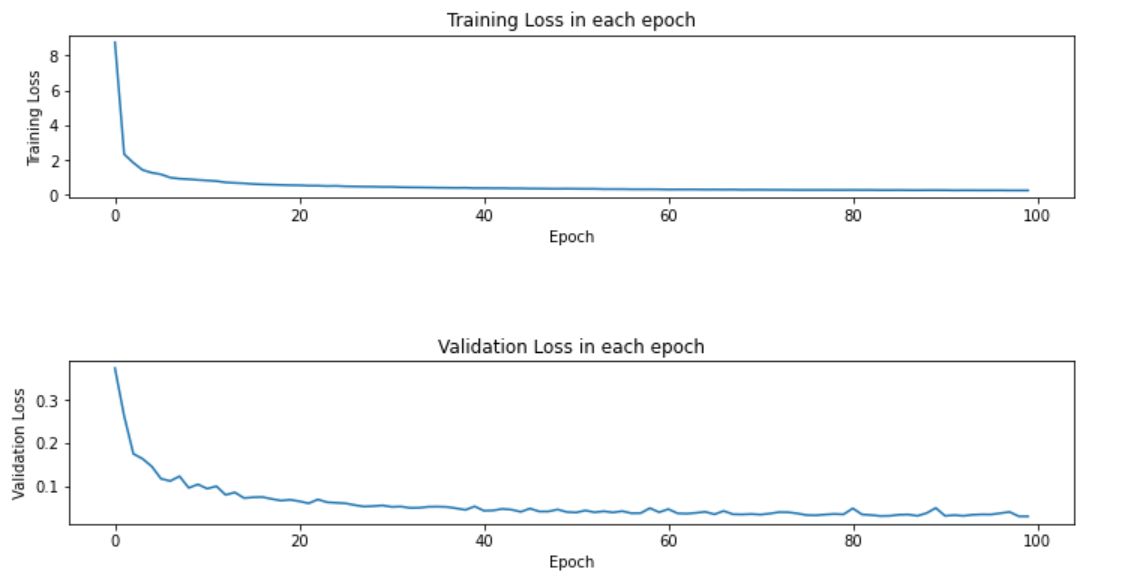
\includegraphics[scale=0.6]{figures/mantle_convection_images/larger_dataset/LSTM_trainingData.png}
    \label{figure:LSTM_larger_losses}
\end{figure}

\begin{figure}[H]
    \caption{Overall testing result of LSTM trained with Larger Dataset.}
    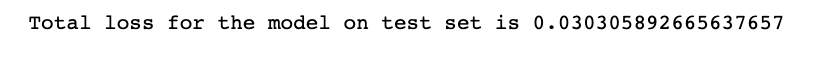
\includegraphics[scale=0.8]{figures/mantle_convection_images/larger_dataset/LSTM_OverallTesting.png}
    \label{figure:LSTM_larger_testing}
\end{figure}

\begin{figure}[H]
    \caption{Ground truth, ground truth after ConvAE's compression-decompression, and most accurate prediction of LSTM trained with Larger Dataset.}
    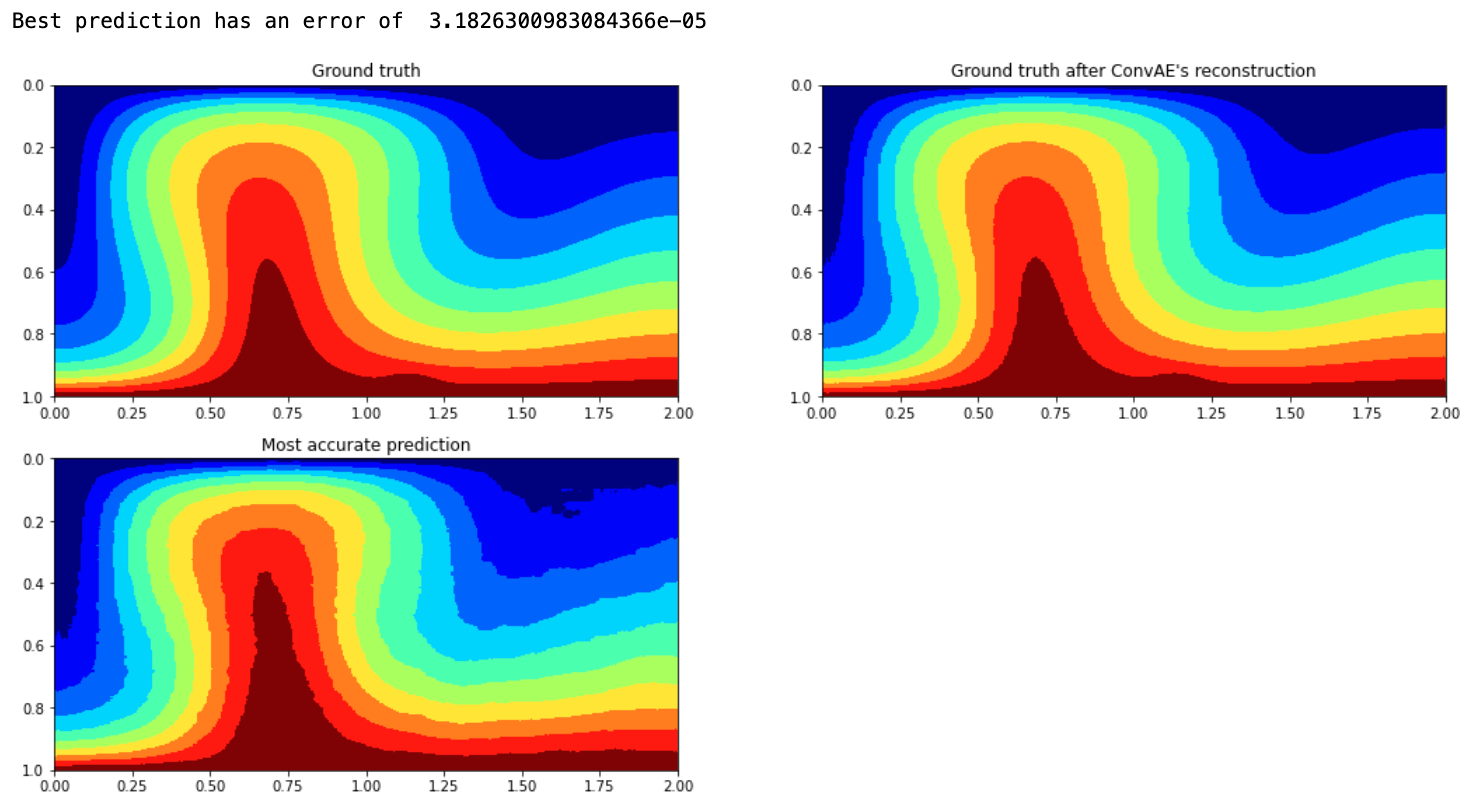
\includegraphics[scale=0.5]{figures/mantle_convection_images/larger_dataset/LSTM_Best.png}
    \label{figure:LSTM_larger_best}
\end{figure}

\begin{figure}[H]
    \caption{Ground truth, ground truth after ConvAE's compression-decompression, and least accurate prediction of LSTM trained with Larger Dataset.}
    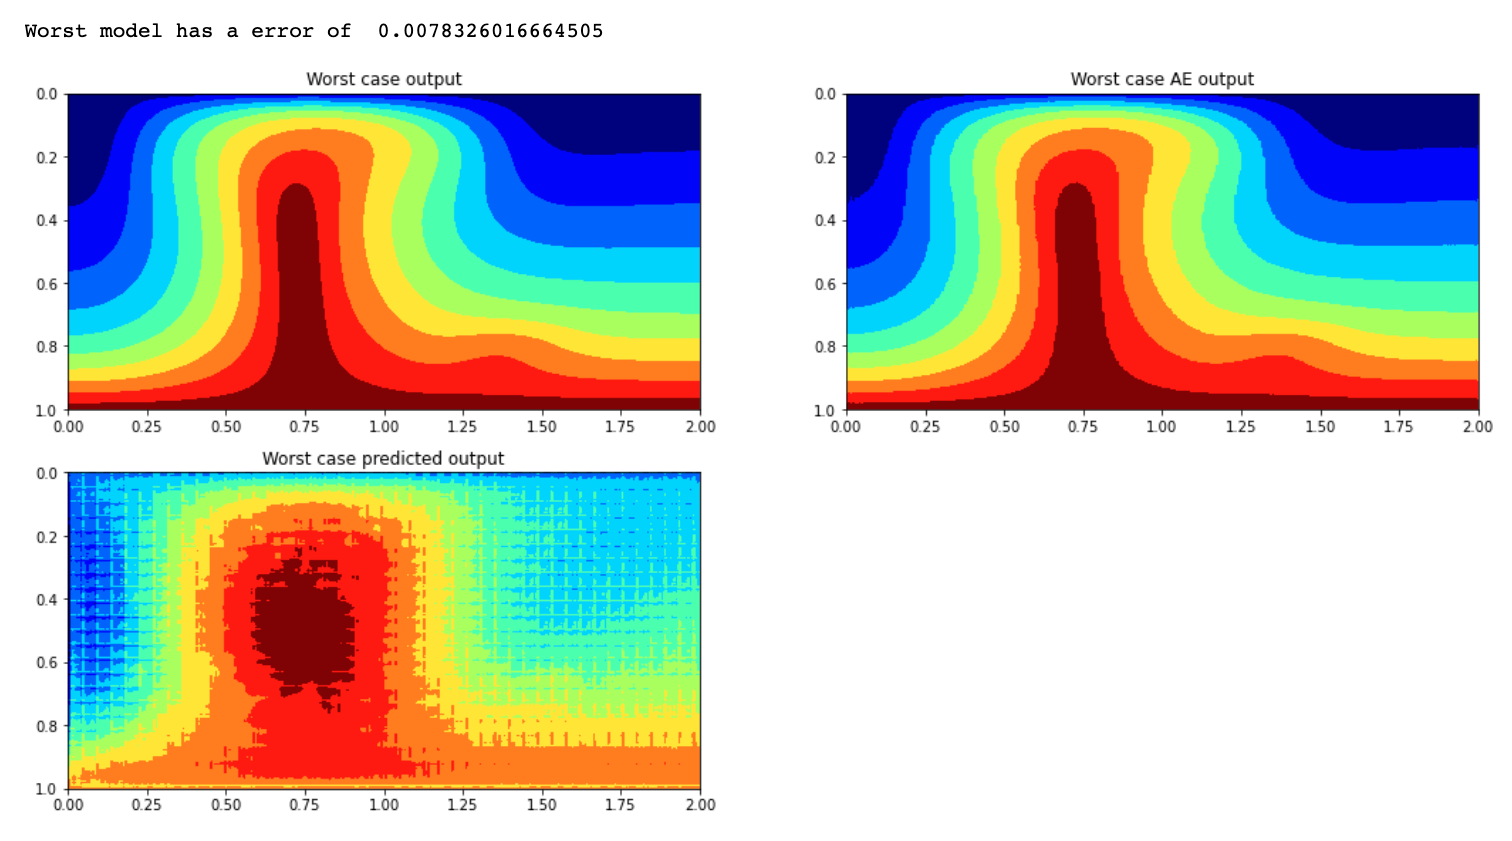
\includegraphics[scale=0.5]{figures/mantle_convection_images/larger_dataset/LSTM_Worst.png}
    \label{figure:LSTM_larger_worst}
\end{figure}


From the above figures, we can see that the loss of the best and worst cases for this LSTM are of the same order as the ones obtained with with the limited dataset given 10 times of the training data, which means that the low accuracy of LSTM is not caused by some potential underfitting problem as discussed in the last section.

For better visualisation, two animations representing the best and worst cases when predicting the rest of the simulation using the first 50 temperature fields are generated.

Figure \ref{figure:LSTM_larger_best_gif} and \ref{figure:LSTM_larger_worst_gif} show 20\% of the two sprite sheets converted from the original animation fields (Every 5th frame).

\begin{figure}[H]
    \centering
    \caption{Best case animation sheet of LSTM trained with Larger Dataset (Link to animation: \url{https://drive.google.com/file/d/1UFYSPVLT1wRsKM5GAdCz0JQLZF8OKNUc/view?usp=sharing})}
    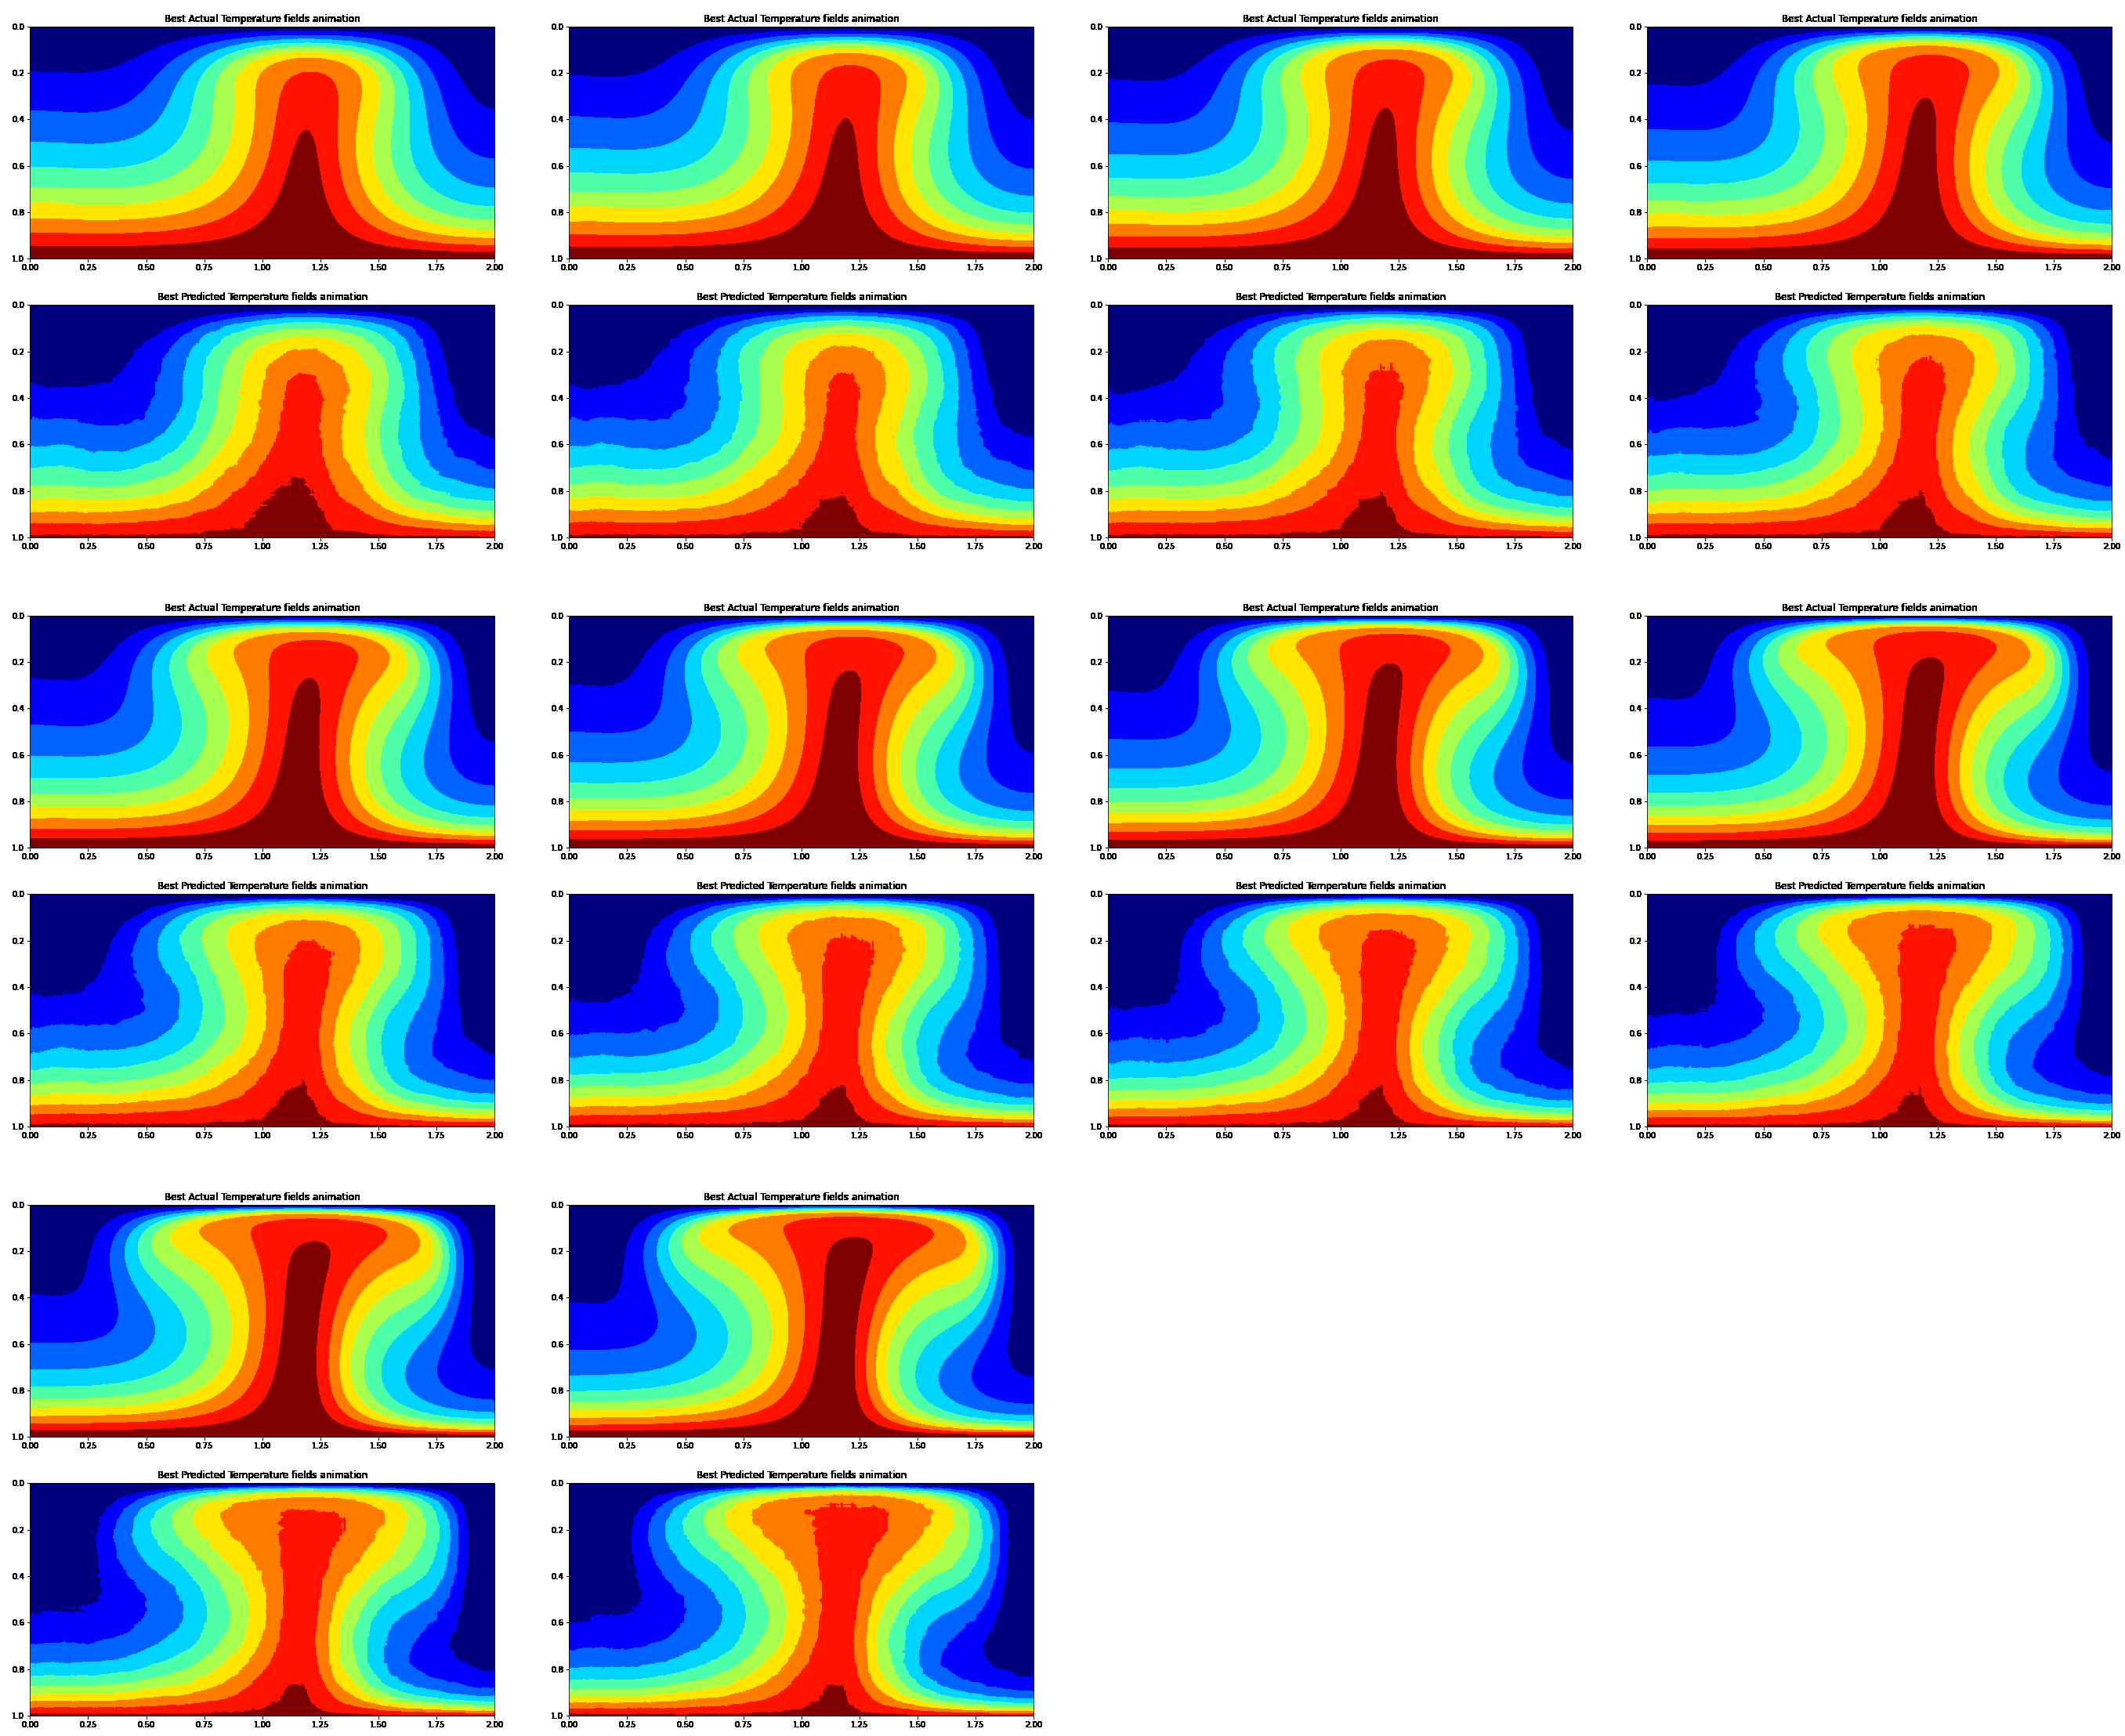
\includegraphics[scale=0.10]{figures/mantle_convection_images/larger_dataset/LSTM_Best_GIF_sheet.png}
    \label{figure:LSTM_larger_best_gif}
\end{figure}



\begin{figure}[H]
    \centering
    \caption{Worst case animation sheet of LSTM trained with Larger Dataset (Link to animation: 
    \url{https://drive.google.com/file/d/1SbzjPwwe7FCu7JCJru8UYHOu9j6uVfZd/view?usp=sharing})}
    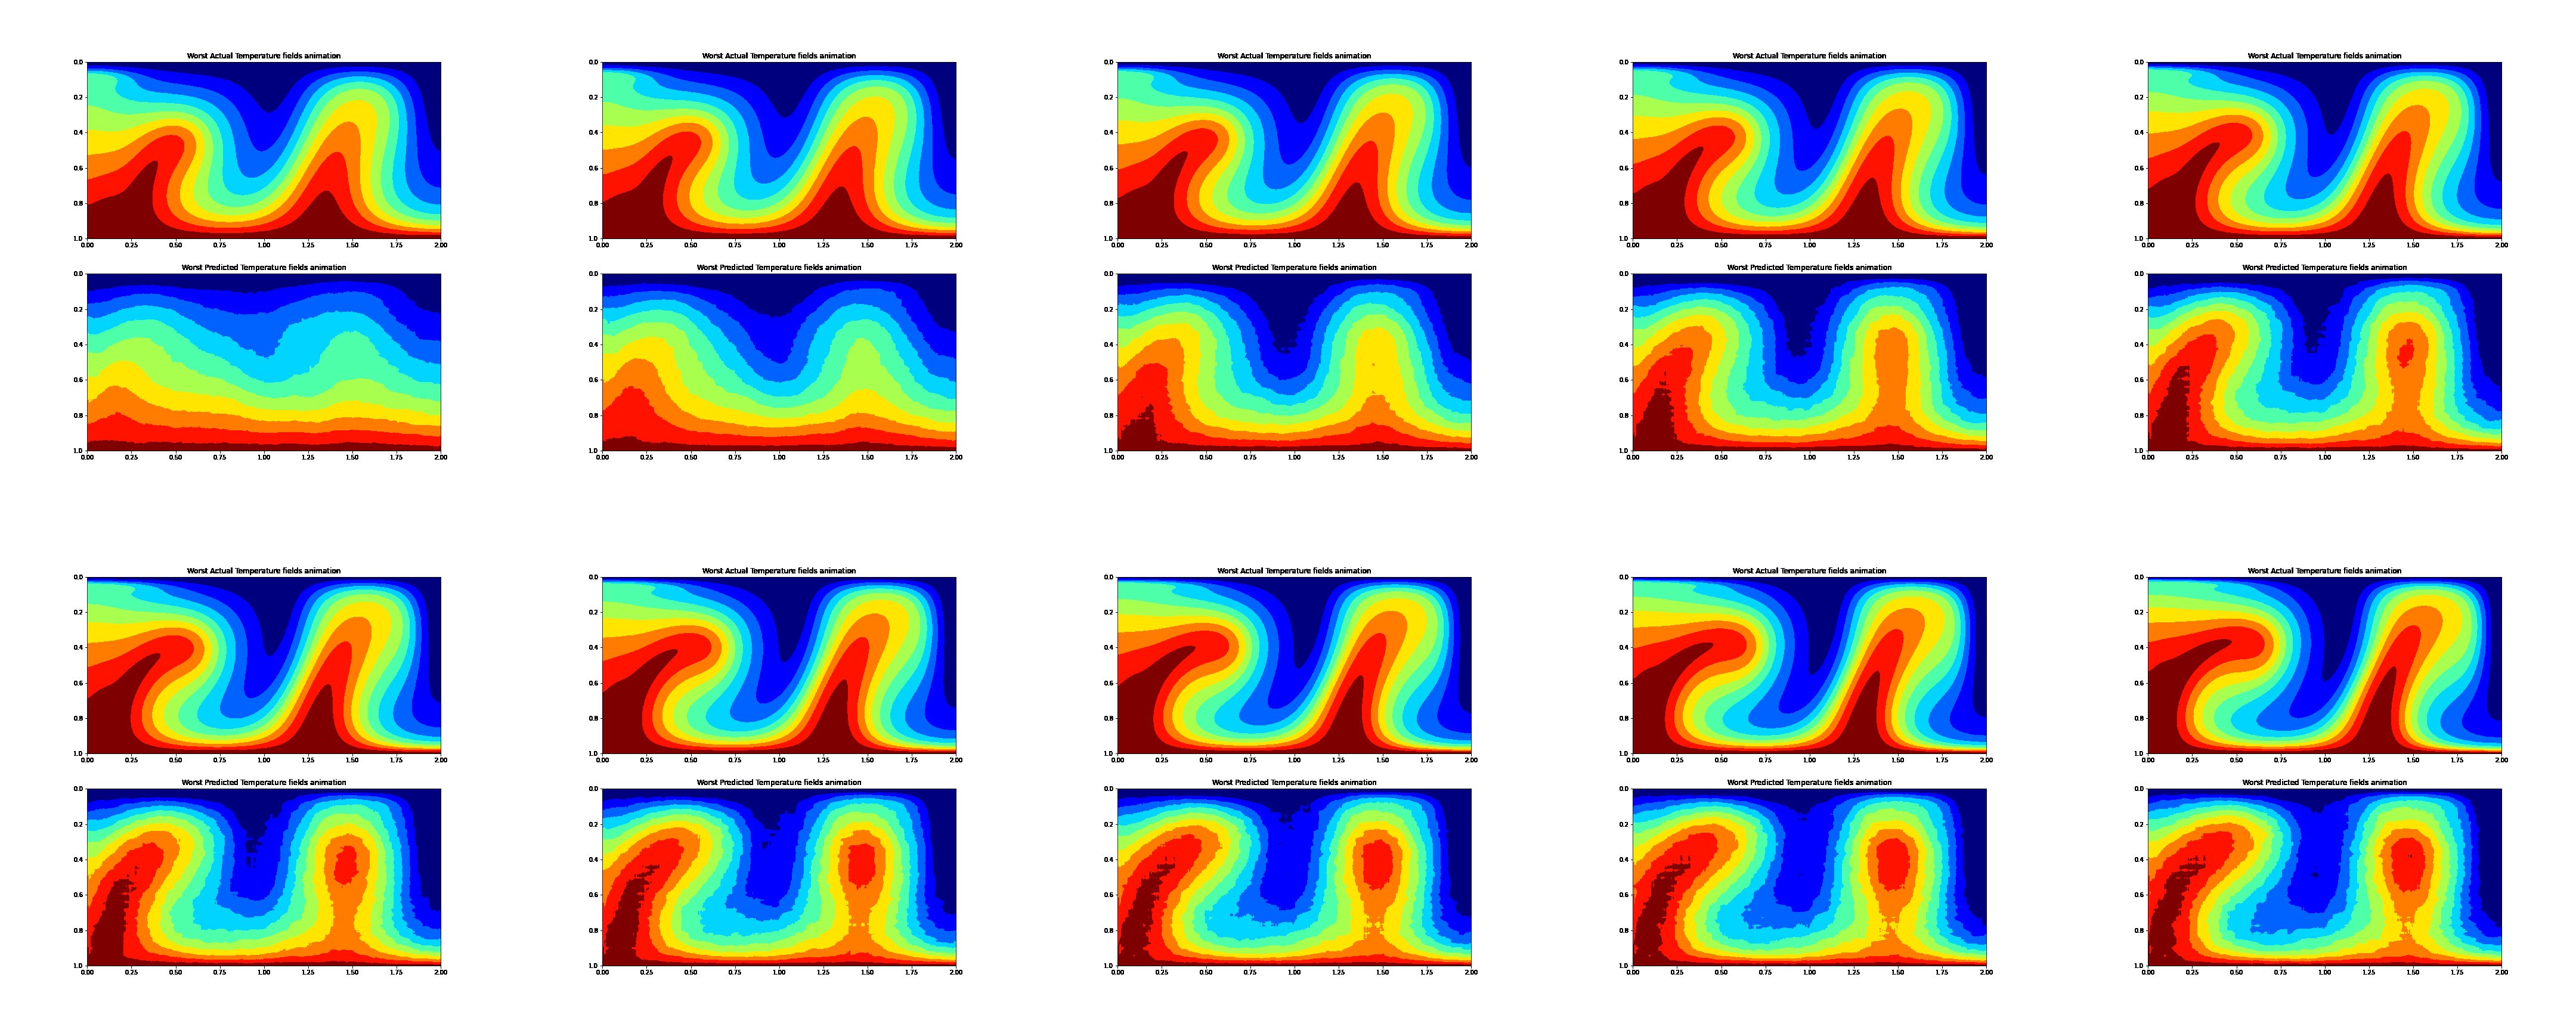
\includegraphics[scale=0.10]{figures/mantle_convection_images/larger_dataset/LSTM_Worst_GIF_sheet.png}
    \label{figure:LSTM_larger_worst_gif}
\end{figure}

POD result for the best and worst cases are shown in Figure \ref{figure:LSTM_larger_best_POD} and \ref{figure:LSTM_larger_worst_POD}, respectively.

\begin{figure}[H]
    \caption{Best case POD of LSTM trained with Larger Dataset.}
    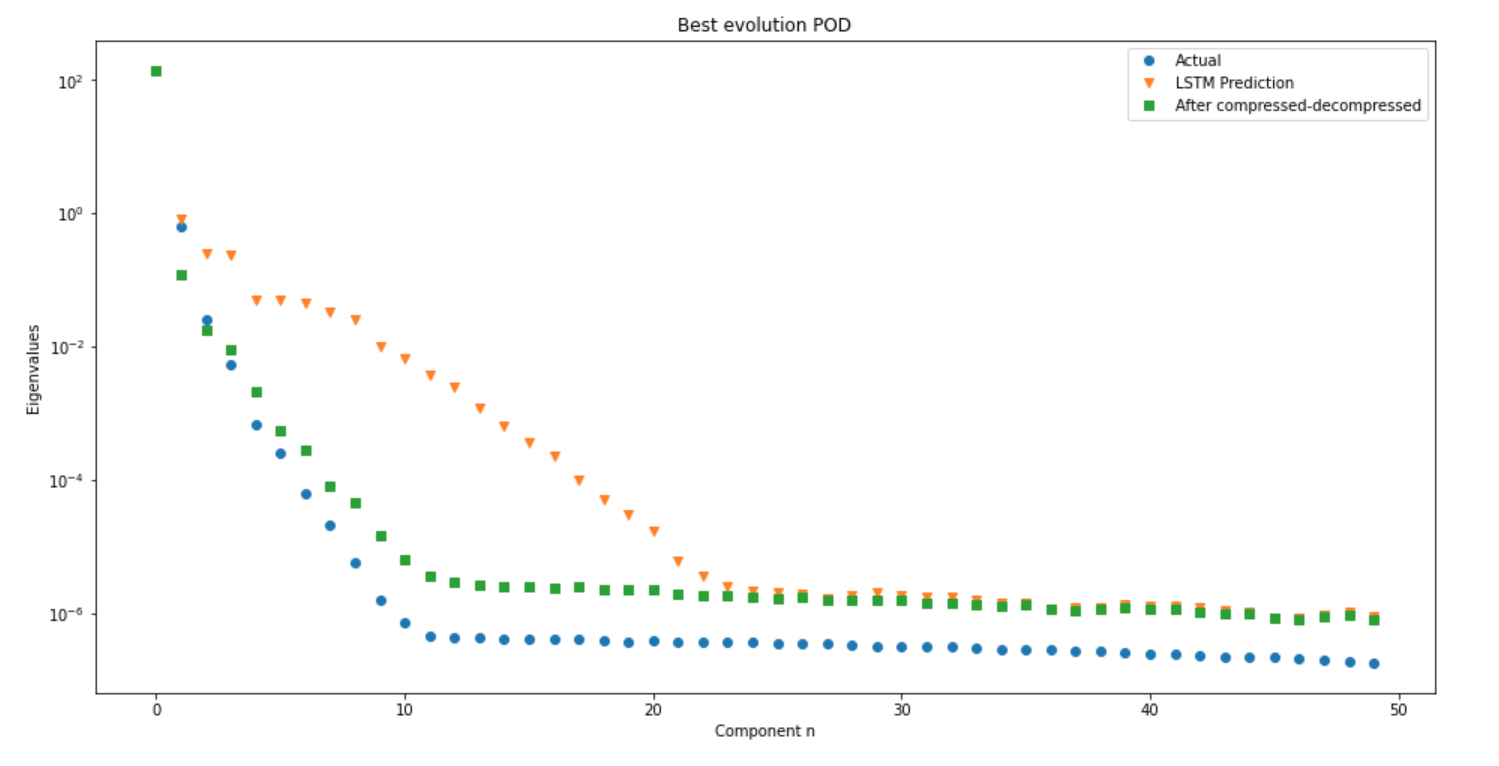
\includegraphics[scale=0.5]{figures/mantle_convection_images/larger_dataset/LSTM_Best_POD.png}
    \label{figure:LSTM_larger_best_POD}
\end{figure}

\begin{figure}[H]
    \caption{Worst case POD of LSTM trained with Larger Dataset.}
    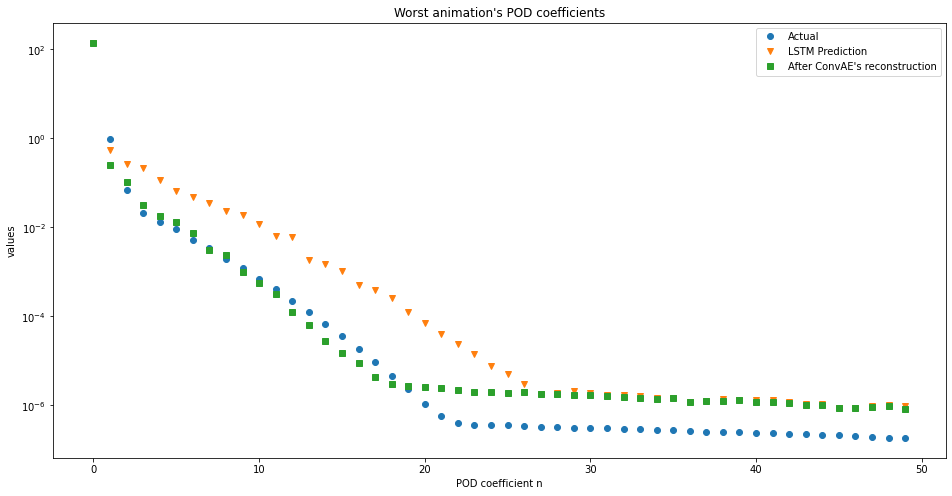
\includegraphics[scale=0.5]{figures/mantle_convection_images/larger_dataset/LSTM_Worst_POD.png}
    \label{figure:LSTM_larger_worst_POD}
\end{figure}

From the animations and the POD results, we can now confirmed that LSTM is able to capture most of characteristics of the simulations even in its worst case and the simulations predicted using LSTM are less accurate compared with those predicted using FNN.


\section{Mantle Convection Simulation on Interpolated Dataset}

To confirm if the problem of the predicted temperature time series moving too fast or too slow is caused by the varying distance between time steps, an interpolated dataset is created using the larger dataset in the last section.

The interpolation process is done for each of the simulation separately by generating a sequence of temperature fields with equal distance between their consecutive time steps. The resulting sequence of time steps for every interpolated simulation are the same by giving a start time step (close to the minimum time step), an end time step (close to the maximum time step) and the number of samples (=100) to generate a new evenly spaced time step sequence to interpolate with. In order to retrieve the temperature field at the target time step, the temperature fields at two nearest time steps are searched for and the target temperature field is generated by linearly interpolating between these two temperature fields.

One thing to notice is that the interpolation may in fact be not physical (not dictated by the physical equations of the system). However, since this experiment is designed to predict temperature field ``like'' evolution with a fixed time step to understand improvements possible if we had regular time steps, 

After the interpolation process, we are able to get an interpolated dataset where every simulation has the same time steps.

The interpolated dataset is also randomly divided in the same way as the limited dataset for each of the three ML architectures in the following subsections.


\subsection{Compression of temperature fields}

The ConvAE used for compressing the temperature fields in this section has the same structure and the same set of hyperparameters as the one trained with the original larger dataset.

In the following figures, some detailed test results from this ConvAE trained with interpolated dataset are presented, including the training and validation losses from Figure \ref{figure:ConvAE_interpolated_losses}, overall testing result from Figure \ref{figure:ConvAE_interpolated_testing}, and the most/least accurate prediction in Figure \ref{figure:ConvAE_interpolated_best_worst}.


\begin{figure}[H]
    \caption{Training and validation losses of ConvAE trained with Interpolated Dataset.}
    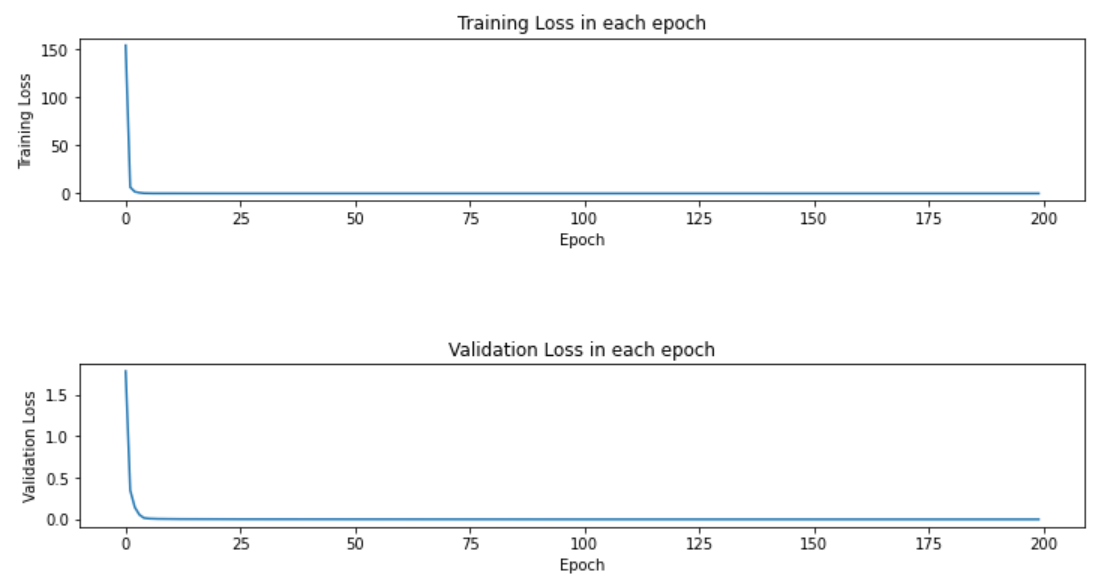
\includegraphics[scale=0.6]{figures/mantle_convection_images/larger_dataset_interpolated/ConvAE_trainingData.png}
    \label{figure:ConvAE_interpolated_losses}
\end{figure}

\begin{figure}[H]
    \caption{Overall testing result of ConvAE trained with Interpolated Dataset.}
    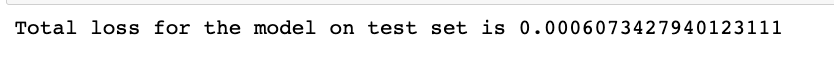
\includegraphics[scale=0.8]{figures/mantle_convection_images/larger_dataset_interpolated/ConvAE_OverallTesting.png}
    \label{figure:ConvAE_interpolated_testing}
\end{figure}

\begin{figure}[H]
\centering
\begin{subfigure}{0.45\textwidth}
    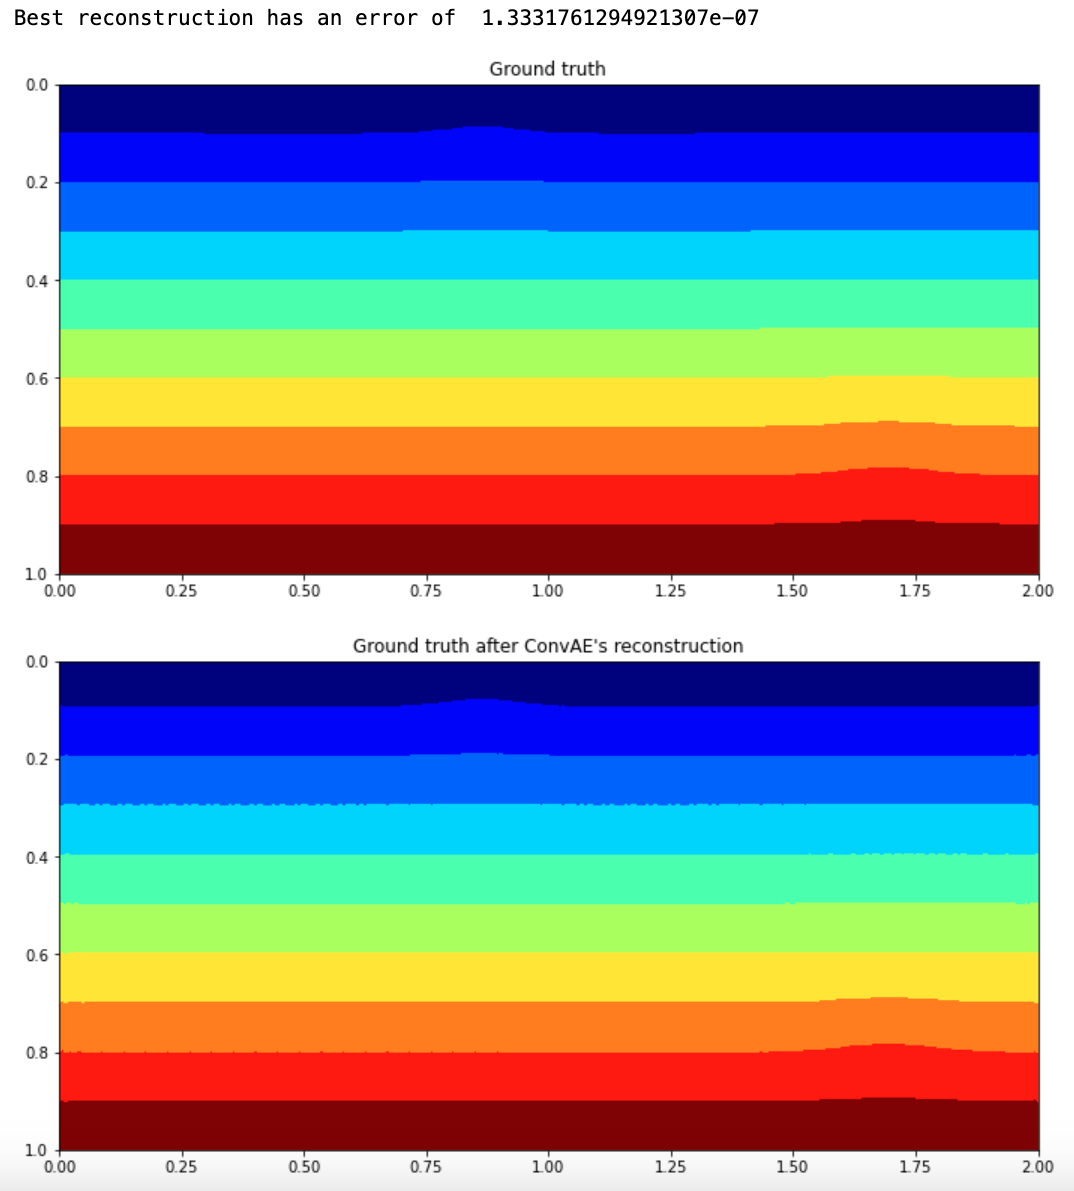
\includegraphics[width=\textwidth]{figures/mantle_convection_images/larger_dataset_interpolated/ConvAE_Best.png}
    \caption{Most accurate reconstruction of ConvAE trained with Interpolated Dataset.}
\end{subfigure}
\hfill
\begin{subfigure}{0.45\textwidth}
    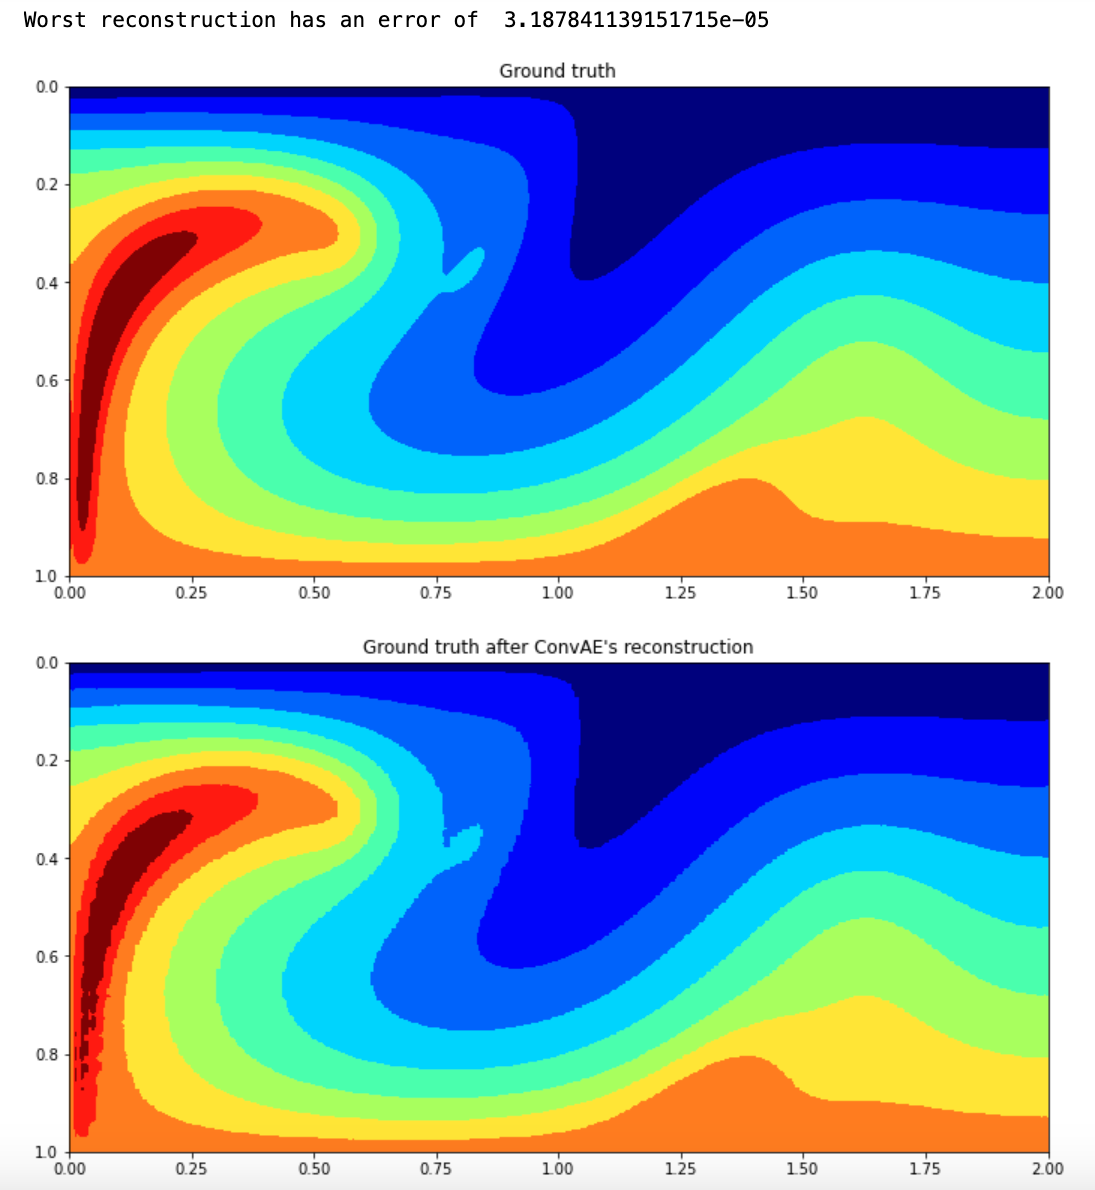
\includegraphics[width=\textwidth]{figures/mantle_convection_images/larger_dataset_interpolated/ConvAE_Worst.png}
    \caption{Least accurate reconstruction of ConvAE trained with Interpolated Dataset.}
\end{subfigure}
\caption{Best case and worst case using ConvAE.}
\label{figure:ConvAE_interpolated_best_worst}
\end{figure}

We can observe that the performance of this ConvAE is better than the one trained with the original larger dataset since it has a total loss that is 3 times lower than the one in the last section (0.0005 to 0.0016). This could imply that the interpolated data makes the training process of ConvAE easier given the same size of data. 


\subsection{Fully Connected Neural Network for Prediction}

The FNN in this section also has the same structure and the same set of hyperparameters as the one trained with the original larger dataset.

The results are presented in the following figures, including the training and validation losses from Figure \ref{figure:FNN_interpolated_losses}, overall testing result from Figure \ref{figure:FNN_interpolated_testing}, and the most/least accurate prediction in Figures \ref{figure:FNN_interpolated_best} and \ref{figure:FNN_interpolated_worst}.

\begin{figure}[H]
    \caption{Training and validation losses of FNN trained with Interpolated Dataset.}
    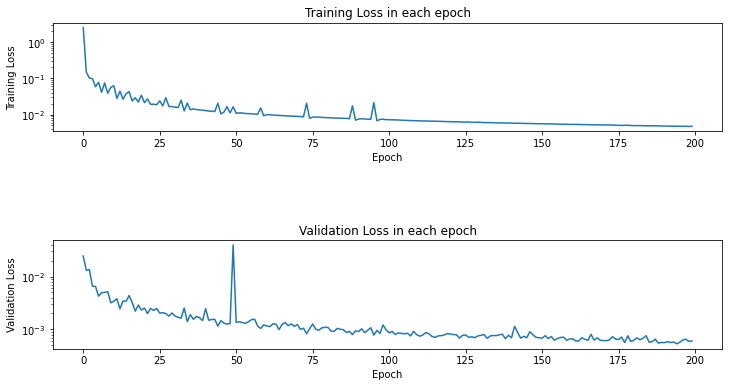
\includegraphics[scale=0.6]{figures/mantle_convection_images/larger_dataset_interpolated/FNN_trainingData.png}
    \label{figure:FNN_interpolated_losses}
\end{figure}

\begin{figure}[H]
    \caption{Overall testing result of FNN trained with Interpolated Dataset.}
    \includegraphics[scale=0.8]{figures/mantle_convection_images/larger_dataset_interpolated/FNN_OverallTesting.png}
    \label{figure:FNN_interpolated_testing}
\end{figure}

\begin{figure}[H]
    \caption{Ground truth, ground truth after ConvAE's compression-decompression, and most accurate prediction of FNN trained with Interpolated Dataset.}
    \includegraphics[scale=0.5]{figures/mantle_convection_images/larger_dataset_interpolated/FNN_Best.png}
    \label{figure:FNN_interpolated_best}
\end{figure}

\begin{figure}[H]
    \caption{Ground truth, ground truth after ConvAE's compression-decompression, and least accurate prediction of FNN trained with Interpolated Dataset.}
    \includegraphics[scale=0.5]{figures/mantle_convection_images/larger_dataset_interpolated/FNN_Worst.png}
    \label{figure:FNN_interpolated_worst}
\end{figure}

The results of FNN are better than the ones trained with the original larger dataset since the loss values are 2 times lower than the one in the last section (0.0005 to 0.0011), which could be partially due to the better performance of the ConvAE.

Again, two animations representing the best and worst cases when predicting the entire simulation using "One-for-All" method (use $T1$ from dataset $\rightarrow$ get predicted $T2$ $\rightarrow$ use predicted $T2$ $\rightarrow$ get predicted $T3$ $\rightarrow$ ...) are generated.

Figures \ref{figure:FNN_interpolated_best_gif} and \ref{figure:FNN_interpolated_worst_gif} show 10\% of the sprite sheets converted from the original animation files (Every 10th frame).

\begin{figure}[H]
    \centering
    \caption{Best case animation sheet of FNN trained with Interpolated Dataset (Link to animation: \url{https://drive.google.com/file/d/10znEe7q_A0rndmuivlbWBH8sZEH6Gv3p/view?usp=sharing})}
    \includegraphics[scale=0.10]{figures/mantle_convection_images/larger_dataset_interpolated/FNN_Best_GIF_sheet.png}
    \label{figure:FNN_interpolated_best_gif}
\end{figure}

\begin{figure}[H]
    \centering
    \caption{Worst case animation sheet of FNN trained with Interpolated Dataset (Link to animation: 
    \url{https://drive.google.com/file/d/1vIXrWn6emumszEy3VDArqdenj3FQeVVa/view?usp=sharing})}
    \includegraphics[scale=0.10]{figures/mantle_convection_images/larger_dataset_interpolated/FNN_Worst_GIF_sheet.png}
    \label{figure:FNN_interpolated_worst_gif}
\end{figure}

Figures \ref{figure:FNN_interpolated_best_POD} and \ref{figure:FNN_interpolated_worst_POD} show the POD result in the best and worst cases, respectively.

\begin{figure}[H]
    \caption{Best case POD of FNN trained with Interpolated Dataset.}
    \includegraphics[scale=0.5]{figures/mantle_convection_images/larger_dataset_interpolated/FNN_Best_POD.png}
    \label{figure:FNN_interpolated_best_POD}
\end{figure}

\begin{figure}[H]
    \caption{Worst case POD of FNN trained with Interpolated Dataset.}
    \includegraphics[scale=0.5]{figures/mantle_convection_images/larger_dataset_interpolated/FNN_Worst_POD.png}
    \label{figure:FNN_interpolated_worst_POD}
\end{figure}

We can observe that the problem of predicted time series moving faster or slower than the actual simulations is now gone. Also, the POD result in the worst case is now closer than the one in the original simulations. This confirmed that the varying time steps are the cause of the inconsistent convection speed and by fixing this issue using an interpolated dataset, the performance of the FNN is improved.


\subsection{Long Short-Term Memory (LSTM) for Prediction}

The LSTM in this section also has the same structure and the same set of hyperparameters as the one trained with the original larger dataset.

The results are presented in the following figures, including the training and validation losses from Figure \ref{figure:LSTM_interpolated_losses}, overall testing result from Figure \ref{figure:LSTM_interpolated_testing}, and the most/least accurate prediction in Figures \ref{figure:LSTM_interpolated_best} and \ref{figure:LSTM_interpolated_worst}, respectively.


\begin{figure}[H]
    \caption{Training and validation losses of LSTM trained with Interpolated Dataset.}
    \includegraphics[scale=0.6]{figures/mantle_convection_images/larger_dataset_interpolated/LSTM_trainingData.png}
    \label{figure:LSTM_interpolated_losses}
\end{figure}

\begin{figure}[H]
    \caption{Overall testing result of LSTM trained with Interpolated Dataset.}
    \includegraphics[scale=0.8]{figures/mantle_convection_images/larger_dataset_interpolated/LSTM_OverallTesting.png}
    \label{figure:LSTM_interpolated_testing}
\end{figure}

\begin{figure}[H]
    \caption{Ground truth, ground truth after ConvAE's compression-decompression, and most accurate prediction of LSTM trained with Interpolated Dataset.}
    \includegraphics[scale=0.5]{figures/mantle_convection_images/larger_dataset_interpolated/LSTM_Best.png}
    \label{figure:LSTM_interpolated_best}
\end{figure}

\begin{figure}[H]
    \caption{Ground truth, ground truth after ConvAE's compression-decompression, and least accurate prediction of LSTM trained with Interpolated Dataset.}
    \includegraphics[scale=0.5]{figures/mantle_convection_images/larger_dataset_interpolated/LSTM_Worst.png}
    \label{figure:LSTM_interpolated_worst}
\end{figure}

From these figures, we can see that the loss of the best case and the average loss of this LSTM is now less than the one trained with the original larger dataset, which means that the interpolation process improves the accuracy when using LSTM as well.

Again, two animations representing the best and worst cases when predicting the rest of the simulation using the first 50 temperature fields are generated.

Figures \ref{figure:LSTM_interpolated_best_gif} and \ref{figure:LSTM_interpolated_worst_gif} show 20\% of the two sprite sheets converted from the original animation files (Every 5th frame).

\begin{figure}[H]
    \centering
    \caption{Best case animation sheet of LSTM trained with Interpolated Dataset (Link to animation: \url{https://drive.google.com/file/d/1fNkJVHw3v8WzVz0IKcPfI9rwmwhYygWS/view?usp=sharing})}
    \includegraphics[scale=0.10]{figures/mantle_convection_images/larger_dataset_interpolated/LSTM_Best_GIF_sheet.png}
     \label{figure:LSTM_interpolated_best_gif}
\end{figure}

\begin{figure}[H]
    \centering
    \caption{Worst case animation sheet of LSTM trained with Interpolated Dataset (Link to animation: 
    \url{https://drive.google.com/file/d/1JbhX4Zznv9YXHZi8IG811495_-YTOq9l/view?usp=sharing})}
    \includegraphics[scale=0.10]{figures/mantle_convection_images/larger_dataset_interpolated/LSTM_Worst_GIF_sheet.png}
    \label{figure:LSTM_interpolated_worst_gif}
\end{figure}

Figures \ref{figure:LSTM_interpolated_best_POD} and \ref{figure:LSTM_interpolated_worst_POD} show the POD results in best case and the worst case, respectively.

\begin{figure}[H]
    \caption{Best case POD of LSTM trained with Interpolated Dataset.}
    \includegraphics[scale=0.5]{figures/mantle_convection_images/larger_dataset_interpolated/LSTM_Best_POD.png}
    \label{figure:LSTM_interpolated_best_POD}
\end{figure}

\begin{figure}[H]
    \caption{Worst case POD of LSTM trained with Interpolated Dataset.}
    \includegraphics[scale=0.5]{figures/mantle_convection_images/larger_dataset_interpolated/LSTM_Worst_POD.png}
    \label{figure:LSTM_interpolated_worst_POD}
\end{figure}


We can observe that the problem of predicted temperature evolution moving faster or slower than the actual simulations is gone, which is consistent with our conclusion in the last subsection.

\section{Further experiments with Fully Connected Neural Network}

To determine experimentally for how many time steps we can use the trained FNN during a set of $S$ consecutive time steps (e.g., $S=2$, $S=4$, or $S=8$, and then ``correct'' the time series with the truth coming from the simulator) without loosing track of the transient dynamics (that is, how large can $S$ be without significantly affecting accuracy), further experiments extending the two methods in the FNN section are done over the entire interpolated dataset using the trained FNN.

To compare against different values of $S$, POD is applied to each generated temperature field sequence to evaluate the difference of the eigenvalues between the predicted simulations and actual simulations. The data loss for each simulation are computed as well. The result for $S = 1, 2, 4, 8, 16, 99$ are shown as below (where $S=1$ is essentially the first method in the FNN section and $S=99$ is the second method), including the data loss shown in Figure \ref{figure:further_loss}, POD difference in Figure \ref{figure:further_POD} and relative POD difference in Figure \ref{figure:further_relative_POD}.

\begin{figure}[H]
    \caption{Data Loss for $S$ consecutive time steps.}
    \includegraphics[scale=0.7]{figures/mantle_convection_images/further_testings/Data_Loss_table.png}
    \label{figure:further_loss}
\end{figure}

\begin{figure}[H]
    \caption{POD difference for $S$ consecutive time steps.}
    \includegraphics[scale=0.7]{figures/mantle_convection_images/further_testings/POD_table.png}
    \label{figure:further_POD}
\end{figure}

\begin{figure}[H]
    \caption{Relative POD difference for $S$ consecutive time steps.}
    \includegraphics[scale=0.7]{figures/mantle_convection_images/further_testings/Relative_POD_table.png}
    \label{figure:further_relative_POD}
\end{figure}

To further evaluate the performance, a series of box plots are drawn, including Figure \ref{figure:further_loss_Box} for the data loss, and Figures \ref{figure:further_POD_Box} and \ref{figure:further_relative_POD_Box} for the POD difference and relative POD difference, respectively.

\begin{figure}[H]
    \caption{Box Plot for data loss when FNN is used in $S$ consecutive time steps before correction.}
    \includegraphics[scale=0.4]{figures/mantle_convection_images/further_testings/Data_Loss_boxplot.png}
    \label{figure:further_loss_Box}
\end{figure}

\begin{figure}[H]
    \caption{Box Plot for POD difference when FNN is used in $S$ consecutive time steps before correction.}
    \includegraphics[scale=0.4]{figures/mantle_convection_images/further_testings/POD_boxplot.png}
    \label{figure:further_POD_Box}
\end{figure}

\begin{figure}[H]
    \caption{Box Plot for relative POD difference when FNN is used in $S$ consecutive time steps before correction.}
    \includegraphics[scale=0.4]{figures/mantle_convection_images/further_testings/Relative_POD_boxplot.png}
    \label{figure:further_relative_POD_Box}
\end{figure}

For better visualisation, the animation representing the ground truth and the predicted simulation using different values of $S$ are shown below in Figure \ref{figure:further_GIF}.

\begin{figure}[H]
    \centering
    \caption{Animation sheet when FNN is used in $S$ consecutive time steps before correction, where $S$ = 1, 2, 4, 8, 16, and 99. The time steps, from left to right, are 1, 25, 50, 75, and 100. (Link to animation: \url{https://drive.google.com/file/d/1XOqXxLkuxnnvaTR0jw-7Sm68IqQFnTFf/view?usp=sharing})}
    \includegraphics[scale=0.30]{figures/mantle_convection_images/further_testings/FNN_further_testing_sheet.png}
    \label{figure:further_GIF}
\end{figure}

One thing that particularly worths pointing out is that the growth of the average data loss with respect to $S$ shown in the box plot is more moderate than expected. Therefore, a plot showing the error growth in loglog is shown as below in Figure \ref{figure:further_loglog}. This enables us to estimate this growth as a function of $S$.

\begin{figure}[H]
    \centering
    \includegraphics[scale=0.4]{figures/mantle_convection_images/further_testings/FNN_LogLog.png}
    \caption{Growth of average data loss with respect to the value of $S$ shown by LogLog, which is approximately $O(0.77S)$.}
    \label{figure:further_loglog}
\end{figure}

We can confirm that when FNN is used during $S$ consecutive time steps, the growth of the data loss with $S$ (ranging from 1, 2, 4, 8, 16 to 99) is remarkably moderate (less than $O(S)$), with only a few outliers deviating moderately from the median. This could provide some avenues for future research.

Overall, we tested on 3 different dataset by using ConvAE to compress the temperature fields and using FNN/LSTM to make predictions. We found that even though FNN using "One-for-One" method is generally better than LSTM when predicting a complete time series for its higher accuracy and lower data loss, LSTM, however, is more capable to capture the characteristic of a simulation than FNN using "One-for-All" method. Inspired by the extremely low computational demands of the "One-for-All" method (1 in, 99 out), we conducted some further evaluaion of FNN when it is used in a series of $S$ consecutive time steps before it is corrected using the ground truth. The result for the growth of the data loss with respect to $S$ is remarkable and could provide some valuable insights for future studies.




